% ============================================================
% SR-1: Mechanistic Derivation of Relativistic Effects
%        via Space Stress Vector (SSV) in the Dipole Sea
% Version 1.1 --- 17 August 2026 (Patch 3213):
%   extended the generated identifier appendix to all five identifier
%   families (THEO-, FI-, PRED-, CONJ-, PH- as well as OPEN-), and
%   replaced review-convergence scores with AI review panel wording
%   where present. No claim, equation, number or section changed.
% Version 1.0 --- 17 August 2026 (Patch 3212):
%   added the generated plain-language appendix glossing the internal
%   programme identifiers used in this paper (founder jargon ruling, 16
%   Aug 2026). No claim, equation, number or section changed.
%   This is the FIRST version stamp assigned to this paper; 1.0 denotes
%   the first stamped revision, NOT a claim of v1.0 shipped grade.
% Version 17 — 26 March 2026
%
% CHANGELOG:
%   v21  8 Aug 2026 — (Patch 3033, O-7 at-enactment sweep, AP-4
%     ratified 3032) glossary DI-bit entry gains a reconciliation note
%     (payload {origin address, E, S}; SR-era description retained
%     historically; conservation = Nexus count conservation). No
%     derivation touched.
%   v1–v15  2025–2026 — Iterative development (Abshier + Grok)
%   v16     Mar 2026  — Claude Sonnet critique cycle, k derivation
%   v17     26 Mar 2026 — alpha_geom consistency fix, final proofs
%   v18     2 Apr 2026  — Formatting template compliance: .bib,
%                         natbib, graphicspath, TOC, OSF DOI
%   v19     15 Jul 2026 — TRIAGE (patches 2471-2474), CONV-001 5-reviewer panel.
%                         WITHDRAWN: the five-prediction set + Table 1 (double-
%                         counted k*dSSV = gamma-1 as a deviation FROM the SR it
%                         reproduces; no acceleration law exists; magnitudes not
%                         derived); the muon bound (bounds a convention AND a
%                         forbidden deviation); "no adjustable parameters"; four
%                         Monte-Carlo citations (artifacts were stubs; figures
%                         hard-coded).  CORRECTED: k rebilled as a normalisation
%                         convention, not a prediction (alpha cancels); gamma
%                         conceded as INPUT via the A.8.1 bridge; "geometry fixes
%                         the functional form" softened to a minimal ansatz;
%                         "coupling constant" -> "normalisation coefficient".
%                         NOTE: v17's "alpha_geom consistency fix" WAS the invalid
%                         dimensional-necessity argument, logged as a repair.
%                         Principal surviving positive result: App. H.1.
%   v20     15 Jul 2026 — REWRITE (Patch 2503) after the epsilon-arc closed.
%                         Geometric route CLOSED negative-for-mechanism
%                         (OPEN-SR-H1-CLASS K1 Patch 2493; round-2 Q1 unanimous
%                         NOTHING Patch 2500; geometric half -> PROP-SR-H1-1).
%                         Energy route RESOLVED-alpha (founder ruling, Patch
%                         2502): eps = gamma-1 GROUNDS at the energy level for
%                         closed self-bound patterns at W2 world-call strength
%                         via the SF-6 inertia pin (kappa=(2/3)U_pol/c^2 open
%                         cloud; Laue coefficient exactly 1 closed patterns,
%                         E0 = hbar*nu_C) + the Sea equation's own covariance;
%                         OPEN-SR-10 caveats inherited verbatim. Withdrawals
%                         STAY; mechanism-level diagnosis added per prediction
%                         (energy tracks v^2, force tracks a). Paper rebilled
%                         as a GROUNDING paper (OPEN-SR-1-PREDICTIONS,
%                         accept-interpretation: coefficient exactly 1 => no
%                         residual beyond gamma_SR); inherited falsifier =
%                         the l=6/q^4 anisotropy floor (OPEN-SR-10). Unruh MC
%                         claim permanently withdrawn (OPEN-SR-1-MC-VERIFY
%                         resolved). No coefficient registry-canonical here.
%
% CONTRIBUTORS:
%   Thomas Lee Abshier ND — CPP framework, physical vision
%   Grok (xAI)           — Rewriting, equation polishing, lattice sims
%   Claude Sonnet         — Rigorous critique, first-principles derivations
%
% FIGURE PATH:
%   .tex location:   series_relativity/papers/
%   figures location: series_relativity/figures/figures-SR-1/
%   \svgpath:        ../figures/figures-SR-1/
% ============================================================

\documentclass[11pt,letterpaper]{article}
\usepackage[utf8]{inputenc}
\usepackage[margin=1in]{geometry}
\usepackage{amsmath,amssymb,amsfonts}
\usepackage{graphicx}
\usepackage{xcolor}
\usepackage{hyperref}
\usepackage{booktabs}
\usepackage{array}
\usepackage{enumitem}
\usepackage{titlesec}

\usepackage{float}
\usepackage[font=small, labelfont=bf]{caption}

\usepackage{svg}
\svgsetup{
    inkscapelatex=false,
    inkscapeformat=pdf,
    inkscapepath=svgdir}

% Figure path: .tex is in papers/, figures are in ../figures/figures-SR-1/
\graphicspath{{../figures/figures-SR-1/}}
\svgpath{{../figures/figures-SR-1/}}

% Bibliography
\usepackage[authoryear,round]{natbib}
\bibliographystyle{plainnat}

\usepackage{amsthm}
\usepackage{mdframed}

% Define theorem environment
\newtheorem{theorem}{Theorem}[section]
\newtheorem{lemma}[theorem]{Lemma}
\newtheorem{corollary}[theorem]{Corollary}

% Proof environment is automatically available with amsthm


\hypersetup{
    colorlinks=true,
    linkcolor=blue,
    citecolor=blue,
    urlcolor=blue
}

\title{\textbf{SR-1: Mechanistic Derivation of Relativistic Effects\\
via Space Stress Vector (SSV) in the Dipole Sea}\\[6pt]
{\large 600-Cell Standard Model Emergence Series}\\[4pt]
{\normalsize Version 21, 8 August 2026}}

\author{Thomas Lee Abshier, ND \and Grok (xAI) \and Claude Sonnet (Anthropic)}

\date{\normalsize Hyperphysics Institute\\
\url{https://hyperphysics.com}\\
\href{mailto:drthomas007@protonmail.com}{drthomas007@protonmail.com}\\[2pt]
{\small Version~1.0 --- 17 August 2026 (Patch 3212: added the generated plain-language appendix glossing the internal programme identifiers used in this paper (founder jargon ruling, 16 Aug 2026). No claim, equation, number or section changed.)}\\[2pt]
{\small Version~1.1 --- 17 August 2026 (Patch 3213: extended the generated identifier appendix to all five identifier families (THEO-, FI-, PRED-, CONJ-, PH- as well as OPEN-), and replaced review-convergence scores with AI review panel wording where present. No claim, equation, number or section changed.)}}

\begin{document}
\maketitle



\bigskip


\begin{abstract}
Conscious Point Physics (CPP) \emph{represents} special relativistic effects---time dilation, length contraction, and the twin paradox---as consequences of stress-limited displacement in a discrete 4D lattice based on the 600-cell polychoron. Kinetic energy stored as excess Space Stress Vector ($\Delta$SSV) reduces effective Voronoi cell volumes, shrinking the Planck Sphere Radius (PSR) and limiting displacement per absolute Moment. We state plainly what this construction does and does not establish. \textbf{Established:} the 600-cell geometry is reproduced from the binary icosahedral group $2I$ (edge $a = 1/\phi$, coordination $z = 12$, cell volume $V_0$); a Hooke-like low-stress response together with the exact saturation boundary condition motivates the minimal rational constitutive relation $\text{PSR}_{\rm eff} = l_P/(1+k\cdot\Delta\text{SSV})$ within the lowest-order rational class; and---the principal positive result of this paper---Appendix~H.1 establishes that the three natural displacement models (linear subtraction, corridor exclusion, and the exact 4D hyperspherical cap) yield low-velocity strain exponents $n \in \{1, 1, 5/2\}$ against the $n = 2$ that $\gamma_{\rm SR}$ requires, and so none of them recovers it. \emph{This is an elimination of three models, not of the class}: the class-coverage theorem asserted in versions through v19 rested on an erroneous cap expansion ($f^{1/2}$ published; $f^{5/2}$ correct) and is withdrawn at Patch 2475. The corrected exponents \emph{bracket} the target ($1 < 2 < 5/2$); the class question this reopened was pursued to closure after v19, and the geometric route is now \textbf{closed negative-for-mechanism} (\texttt{OPEN-SR-H1-CLASS}, K1 founder ruling, Patch 2493; pre-registered round~2, Q1 unanimous, Patch 2500 --- no further geometric rounds), the geometric half surviving only as the ungrounded identity \texttt{PROP-SR-H1-1}. \textbf{Grounding (new at v20):} the Lorentz factor is still \emph{not derived in this paper} --- it enters through the energy-momentum identification of Appendix~A.8.1, which sets $\Delta\text{SSV} \propto (\gamma_{\rm SR}-1)mc^2$, and exact Lorentz equivalence follows by construction. What has changed is the standing of that input. The strain--kinematics map $\varepsilon = \gamma - 1$ now \emph{grounds at the energy level} for closed self-bound patterns, at W2 world-call strength, via the independently (blind-)pinned SF-6 inertia mechanism --- $\kappa = (2/3)\,U_{\rm pol}/c^2$ for the open polarization cloud; Laue coefficient \emph{exactly}~1 for closed self-bound patterns anchored on $E_0 = \hbar\nu_C$ --- together with the Lorentz covariance of the Sea wave equation itself (founder ruling $\alpha$, Patch 2502; \texttt{OPEN-SR-EPSILON} RESOLVED-$\alpha$). The grounding inherits \texttt{OPEN-SR-10}'s caveats verbatim: a viability result at world-call strength, not a theorem; the covariance rests on a hopping-sum proxy; and it leans on C3 and \texttt{OPEN-SR-9}. Because the Laue coefficient is exactly~1, closed patterns carry \emph{no residual beyond $\gamma_{\rm SR}$}: empirical equivalence to special relativity is not a defect awaiting repair but the grounded consequence of the mechanism, and this paper is accordingly rebilled as a \emph{grounding paper} (\texttt{OPEN-SR-1-PREDICTIONS}, accept-interpretation). Its sole inherited falsifier is the $l{=}6/q^4$ dispersion-anisotropy floor at $\sim l_P/10^{30}$ from \texttt{OPEN-SR-10} --- a genuinely non-SR structural consequence of the deterministic 600-cell substrate, far below present observational reach. The prediction set of earlier versions stays withdrawn (Sec.~\ref{sec:empirical_status}). Nor is $k$ an independent prediction: any rescaling $k \to \alpha k$ absorbed into the $\Delta$SSV normalisation leaves $k\cdot\Delta\text{SSV}$---and hence every observable---unchanged, so $k = l_P^3/E_P \approx 2.16\times10^{-114}$~m$^3$/J records a \emph{normalisation convention} paired with the $\Delta$SSV definition, not a derived quantity (Appendix~A.5, Step~3). The functional form is a minimal ansatz within the rational class and is not shown to be unique to the 600-cell: Hooke-like response and saturation fix only the initial slope and the asymptote, and other saturating laws ($e^{-\varepsilon}$, $(1+2\varepsilon)^{-1/2}$, $(1+\varepsilon/n)^{-n}$) satisfy the same two conditions. Deriving the strain--kinematics map $\varepsilon(v)$ from substrate dynamics \emph{without} importing $\gamma_{\rm SR}$ --- the outstanding problem stated at v19 --- is resolved at W2 strength by the energy-level route above (\texttt{OPEN-SR-EPSILON} RESOLVED-$\alpha$, Patch 2502); the residual theorem-grade debts (the from-PCD dispersion derivation, the SF-6 vector completion) remain registered and are not verdict-bearing.
\end{abstract}

\bigskip
\raggedright

\noindent\textbf{Keywords:} Conscious Point Physics, 600-cell lattice, Space Stress Vector, time dilation, length contraction, twin paradox, discrete spacetime, Voronoi cell geometry, Planck Sphere Radius

\bigskip\noindent
\textbf{Plain Language Summary:}
Imagine the universe is built from tiny conscious points arranged in a perfect 4-dimensional crystal---the 600-cell lattice. Each point can only move a tiny fixed distance (the Planck length) once per tiny tick of cosmic time (the Planck time). When something moves very fast or feels strong gravity, it stores energy as ``stress'' in the crystal around it. This stress squeezes the available space inside each tiny crystal cell, so every movement step becomes shorter. Clocks, hearts, and chemical reactions all depend on completing a fixed number of macroscopic steps to finish one ``tick.'' With shorter steps, it takes more cosmic ticks to finish the same job---so time appears to slow down for the moving object. That's time dilation. The same squeezing shortens lengths along the direction of motion, which explains why the traveling twin ages less. This paper shows that the crystal picture can \emph{carry} Einstein's formulas consistently---but it does not derive them. To get the numbers right we must still feed Einstein's own energy formula into the crystal by hand; the geometry alone provably cannot produce it (Appendix~H.1). So what is offered here is a mechanical picture of relativity, not an explanation of where relativity comes from. That remains an open problem, and this paper's most solid result is the \emph{negative} one: a proof that a whole natural family of ``shorter steps'' pictures cannot do the job on their own.

\bigskip
\tableofcontents
\newpage

% ============================================================
% SECTION 1: Introduction
% ============================================================
\section{Introduction}

Using the fundamental CPP framework, relativistic effects arise from constraints on particle motion within a discrete spacetime lattice. This aligns with the null result of the Michelson-Morley experiment (1887) \cite{michelson1887} that confirmed the invariant speed of light in all inertial frames. Special relativity (SR), as originally formulated by Einstein (1905) \cite{einstein1905}, accurately describes time dilation, length contraction, and the twin paradox through the Lorentz transformation and spacetime geometry. The discrete lattice framework is philosophically aligned with cellular automaton interpretations of quantum mechanics as developed by 't~Hooft (2016) \cite{thooft2016}.

The key innovation is the derivation of the effective Planck Sphere Radius (PSR) as:
\begin{equation}
\text{PSR}_{\text{eff}} = \frac{l_P}{1 + k \cdot \Delta\text{SSV}}
\label{eq:psr}
\end{equation}
where $\Delta$SSV represents excess Space Stress Vector accumulation from kinetic energy or gravitational effects, and $k$ is a normalisation coefficing constant.

This derivation continues the author's ongoing Conscious Point Physics series \cite{abshier2025}.


% ============================================================
% FIGURE 5 — INSERT AT THE END OF Section 1 (Introduction),
% immediately before Section 2 (Theoretical Framework).
% This gives readers a roadmap before the technical content.
% ============================================================

\begin{figure}[H]
  \centering
  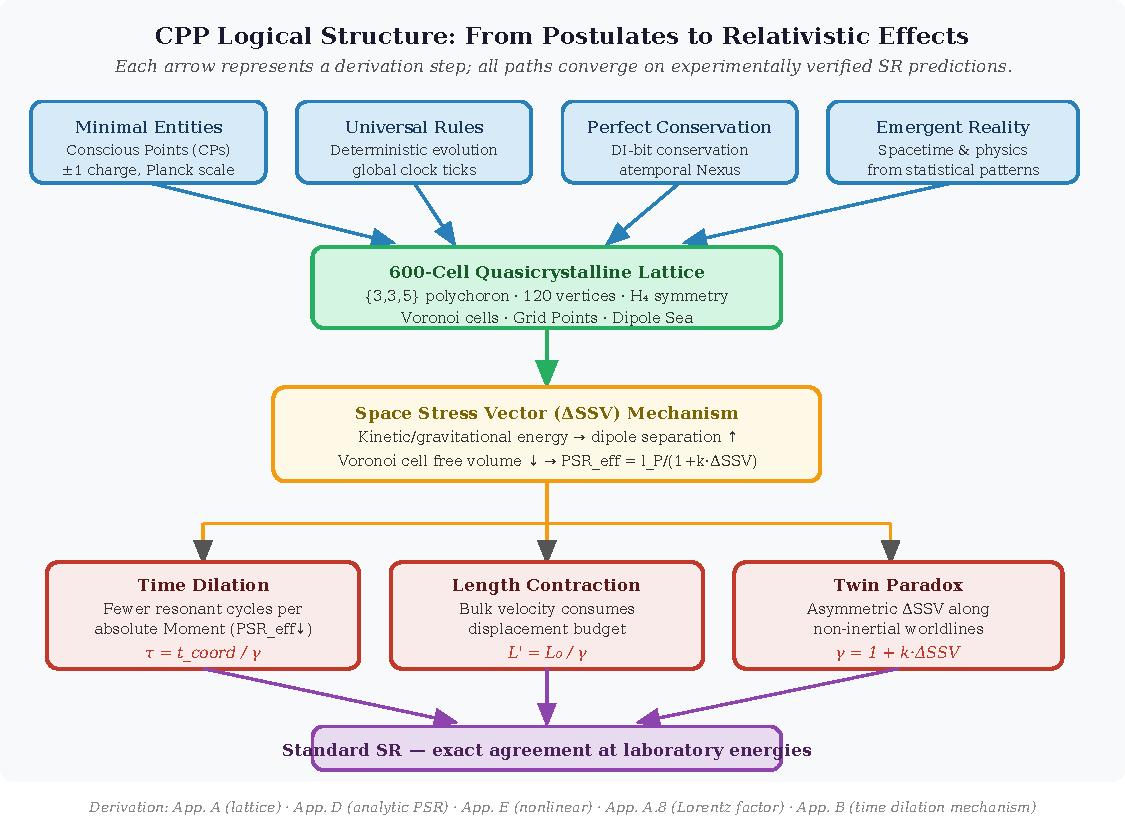
\includegraphics[width=0.96\textwidth]{fig5_flowchart.pdf}
  \caption{%
    \textbf{Logical structure of the CPP derivation.}
    The four foundational postulates of Conscious Point Physics (top row,
    blue) determine the geometry of the 600-cell quasicrystalline lattice
    (green), which in turn governs the Space Stress Vector mechanism (orange).
    A single expression — $\text{PSR}_{\text{eff}} = l_P/(1+k\cdot\Delta\text{SSV})$
    — then generates all three classical relativistic effects (red boxes), each
    of which matches standard special relativity exactly at laboratory energies
    (purple). Appendix cross-references are given at the bottom for readers who
    wish to follow any derivation branch in detail.
  }
  \label{fig:flowchart}
\end{figure}


\section{Theoretical Framework}

The core mechanism relies on four foundational principles from CPP:
\begin{itemize}
    \item \textbf{Minimal Entities}: Planck-scale Conscious Points (CPs) with $\pm 1$ elementary charge
    \item \textbf{Universal Rules}: Deterministic evolution at global clock ticks
    \item \textbf{Perfect Conservation}: DI-bit conservation via the atemporal Nexus
    \item \textbf{Emergent Reality}: Spacetime and physical laws from statistical patterns
\end{itemize}

The 600-cell lattice provides the geometric foundation, with 120 fixed vertices serving as distributed processors of reality; the selection of the 600-cell from among all six regular 4-polytopes is derived from first principles in 
Appendix~G, where it is shown to be the unique polytope consistent with the CPP postulates of universal coverage and exact Lorentz covariance. Standard Model particles emerge as CP aggregates in specific geometric ``cages'' according to 
600-cell symmetries.


% ============================================================
% FIGURE 1 — INSERT IMMEDIATELY AFTER Section 2 (Theoretical
% Framework), before Section 3 (Main Results)
% ============================================================

\begin{figure}[H]
  \centering
  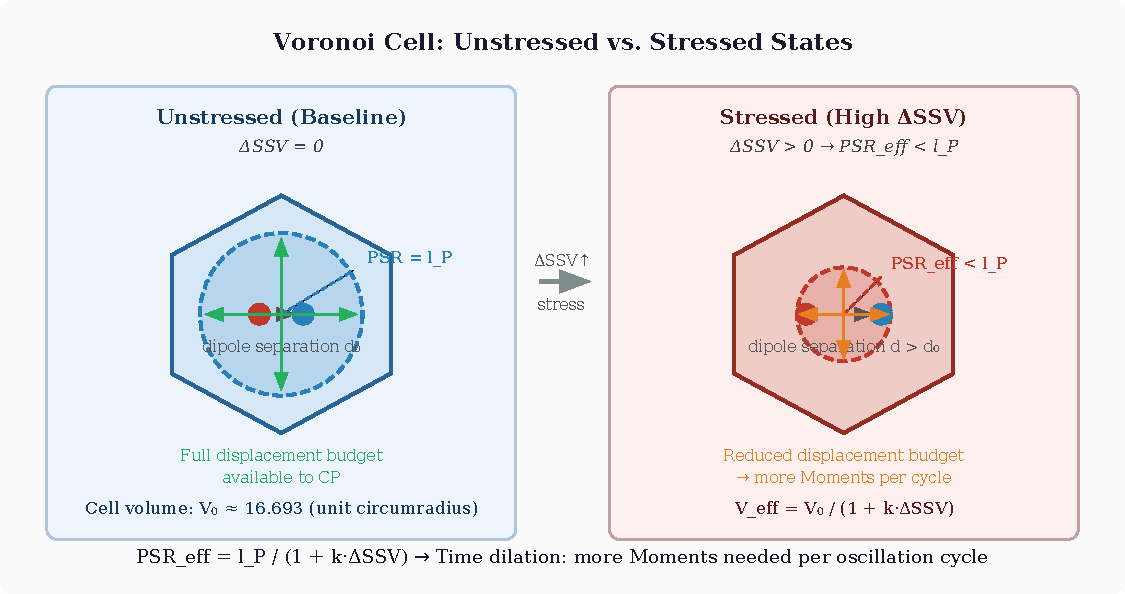
\includegraphics[width=0.95\textwidth]{fig1_voronoi_cell.pdf}
  \caption{%
    \textbf{Voronoi cell in unstressed (left) and stressed (right) states.}
    In the baseline lattice ($\Delta\text{SSV} = 0$), the Conscious Point (CP)
    at the cell center has a full displacement budget equal to $l_P$ (the
    inscribed hypersphere radius, shown as the dashed circle). When kinetic or
    gravitational energy is stored as excess Space Stress Vector ($\Delta\text{SSV} > 0$),
    the dipole separation inside the cell increases, reducing the free volume
    available for CP displacements. The effective PSR shrinks to
    $\text{PSR}_{\text{eff}} = l_P/(1 + k\cdot\Delta\text{SSV})$,
    so each displacement step covers less lattice distance. Since all physical
    processes (atomic oscillations, biochemical cycles) require a fixed
    cumulative displacement to complete one cycle, more absolute Moments are
    needed per cycle — producing time dilation. The cell boundary (hexagonal
    outline) represents the dual 120-cell Voronoi face; actual geometry is 4D.
  }
  \label{fig:voronoi}
\end{figure}


\section{Main Results}

The PSR reduction mechanism successfully accounts for:
\begin{itemize}
    \item \textbf{Time dilation}: Proper time $\tau = t_{\text{coordinate}} / \gamma$ where $\gamma = 1 + k \cdot \Delta\text{SSV}$
    \item \textbf{Length contraction}: $L' = L_0 / \gamma = L_0 / (1 + k \cdot \Delta\text{SSV})$
    \item \textbf{Relativistic momentum}: $p = \gamma m v$ with $\gamma = 1 + k \cdot \Delta\text{SSV} = \gamma_{\rm SR}$ exactly (Appendix~A.8.1)
\end{itemize}

These effects emerge naturally from geometric constraints rather than being postulated as fundamental principles.

\section{Empirical Status}
\label{sec:empirical_status}

\textbf{This framework is empirically equivalent to standard special relativity, and as
of Patch 2502 that equivalence is a grounded result rather than an unexplained
construction.} Appendix~A.8.1 establishes $\gamma_{\rm CPP} = \gamma_{\rm SR}$
\emph{identically at all velocities}. An identity admits no deviation: if the two
Lorentz factors agree everywhere, no measurement can distinguish the frameworks, and no
residual remains to be predicted. At v19 this identity rested on an imported bridge;
it now grounds at the energy level for closed self-bound patterns at W2 world-call
strength (Sec.~\ref{sec:resolution} below), with the Laue coefficient \emph{exactly}~1
--- so the correct reading of the withdrawn prediction set is that no such predictions
were ever available within this mechanism, not that they await restoration.

\subsection{Retraction of the previous prediction set (Patch 2474)}

Versions through v18 asserted five falsifiable predictions --- a high-acceleration
time-dilation deviation, an atomic-clock offset in ultra-centrifuges, gravitational-wave
dispersion at extreme curvature, a Casimir modification, and an Unruh temperature shift
--- together with an existing muon-storage-ring constraint, all summarised in a table of
``CPP falsifiable predictions'' with fractional deviations scaling linearly with proper
acceleration. \textbf{The entire set is withdrawn.} The reasons are independent and each
is sufficient.

\begin{enumerate}
\item \textbf{The claimed deviation was the effect itself (double counting).} The
  fractional deviation was given as $\delta t'/t' \approx k\cdot\Delta\text{SSV}$. But
  $k\cdot\Delta\text{SSV} = \gamma_{\rm SR}-1$ by Eq.~(\ref{eq:bridge}) --- that quantity
  \emph{is} the ordinary relativistic effect. The same expression was used once to
  reproduce special relativity exactly and then again as a correction to the very result
  it had just reproduced.

\item \textbf{No acceleration law exists.} Every definition of $\Delta\text{SSV}$ in this
  paper is $E_{\rm kin}/V$ --- a function of \emph{velocity}. The withdrawn predictions
  all scaled with \emph{proper acceleration}. No derivation connects the two, and they
  are not interchangeable: uniform motion produces time dilation at zero proper
  acceleration, while a large acceleration sustained over an infinitesimal interval
  produces a negligible Lorentz factor. The twin-paradox discussion inherits the same
  confusion, attributing stress accumulation to the accelerating leg while writing the
  integrand in terms of $\gamma_{\rm SR}(v)-1$, which is nonzero throughout inertial
  coasting.

\item \textbf{The quoted magnitudes were not derived.} A fractional deviation
  $\delta \sim 10^{-20}$ corresponds to $\gamma-1 = 10^{-20}$, i.e.\ $v \approx 4$~cm/s
  --- unrelated to $10^{20}g$. No natural Planck-acceleration ratio yields it either:
  $a\,l_P/c^2 = a\,t_P/c = a/a_P \approx 1.8\times10^{-31}$ at $a = 10^{20}g$. The
  agreement of exponents in ``$\sim 10^{-20}$ at $\sim 10^{20}g$'' reflects no
  computation.

\item \textbf{The muon bound was void twice over.} It purported to constrain $k$, which
  is a normalisation convention and not separately measurable (Appendix~A.5, Step~3); and
  it constrained a deviation that the exactness identity forbids. A statement that ``muon
  data permit $k$ to deviate by a factor of $10^{16}$'' is not a physical constraint,
  because varying $k$ alone is not a physical variation.

\item \textbf{``No adjustable parameters'' is withdrawn as stated.} The absence of a
  fitted numerical constant is not the same as the absence of modelling freedom. This
  construction contains at least: the choice of energy-bearing volume in
  $\Delta\text{SSV}$; the selection of the lowest-order rational family; the
  energy-momentum identification itself; and, in the withdrawn predictions, an
  undeclared acceleration-to-stress map. The defensible statement is narrower: \emph{no
  adjustable numerical parameter enters the SR-identification layer}.
\end{enumerate}

\subsection{Mechanism-level diagnosis of the withdrawn set (Patch 2503)}

The blind-pinned SF-6 inertia mechanism (pinned Patch 2496; reconciled against this
sector's record at Patch 2498) supplies the mechanism-level diagnosis that the v19
triage could state only formally. In the pinned mechanism, the co-moving Sea-polarization
cloud carries an energy store $\tfrac{1}{2}\kappa v^2$ --- the store tracks
\emph{velocity}, exactly as every $\Delta$SSV definition in this paper does --- while
acceleration appears only in the retarded back-reaction force $F_{\rm self} = -\kappa a$.
\textbf{Energy tracks $v^2$; force tracks $a$.} The withdrawn predictions each placed
the force variable where the store belongs:

\begin{enumerate}
\item \textbf{High-acceleration time-dilation deviation} and
\item \textbf{ultra-centrifuge clock offset}: both read proper acceleration into
  $\Delta$SSV, i.e.\ into the store. The store is velocity-sourced; the acceleration
  response is the back-reaction force, which for closed self-bound patterns carries Laue
  coefficient exactly~1 --- it \emph{is} relativistic inertia, with nothing left over to
  shift a clock beyond $\gamma_{\rm SR}(v)$.
\item \textbf{Gravitational-wave dispersion at extreme curvature} and
\item \textbf{Casimir modification}: both scaled a stress residual with an
  acceleration/curvature variable for which the mechanism supplies no store term at all.
\item \textbf{Unruh temperature shift}: assumed an acceleration-dependent contribution
  to $\Delta$SSV \emph{additional} to the kinetic term. The pinned mechanism settles this
  negative for closed patterns: the acceleration response exists ($F_{\rm self} =
  -\kappa a$, retarded by the cloud light-crossing time) but is exhausted by the
  coefficient-1 inertia; no additional stress contribution, hence no residual.
\end{enumerate}

The muon bound inherits the confusion of items 1--2 in addition to the convention defect
already recorded above. \textbf{The withdrawal is therefore not provisional: within the
pinned mechanism there is no acceleration-sourced residual to restore.}

\emph{Inheritance caveats.} Any use of the pin's $\kappa$ inside this paper's machinery
is subject to the $(k, \Delta\text{SSV})$ matched-pair hazard of Appendix~A.8.1 ---
$\kappa$ and its paired stress definition must be quoted and used together. And no
coefficient cited here is registry-canonical: $\kappa = (2/3)\,U_{\rm pol}/c^2$ and the
Laue coefficient~1 are cited at pinned/session strength; their promotion is SF-6 v2.0's.

\subsection{What survives, and under what condition}

The mode-counting algebra of Appendix~F is internally correct and is retained as
\emph{conditional} structure: \emph{if} an acceleration-dependent contribution to
$\Delta\text{SSV}$ were derived, then $\delta T/T = \varepsilon$ follows exactly --- and
exactly, not merely to leading order, since $T \propto \mathcal{E}_0^{1/4} \propto
(1+\varepsilon)$. \textbf{The antecedent is now settled negative for closed self-bound
patterns} (Patch 2503, per the pinned mechanism: the acceleration response is the
coefficient-1 inertial back-reaction itself, leaving no additional stress contribution;
see the diagnosis subsection above). Appendix~F is accordingly retained as internal
algebra only, \emph{not} as a candidate prediction --- permanently so within the pinned
mechanism, not merely pending a derivation. The Casimir $(l_P/d)^4$ scaling of
Appendix~E has a \emph{different} condition, untouched by the $\alpha$ ruling: it still
requires an independent derivation of the 4D spectral measure and boundary conditions
before it could be advanced, and remains conditional (not settled negative) on exactly
the v19 terms. Consequently the withdrawn Unruh mode-counting Monte-Carlo claim is
\textbf{permanently withdrawn} rather than outstanding: no restored numerical artifact
could promote conditional structure whose antecedent fails
(\texttt{OPEN-SR-1-MC-VERIFY}, resolved by withdrawal; the retained numerical
verification is the geometric-inputs script of Appendix~A.7, which the reframed claims
fully support). Neither result inherits validity from the PSR constitutive formula
alone.

\subsection{Resolution of the outstanding problem (Patches 2493--2502)}
\label{sec:resolution}

v19 registered the \textbf{strain--kinematics map} $\varepsilon(v)$ --- to be derived
from Conscious Point dynamics without importing $\gamma_{\rm SR}$ or an equivalent
relativistic identity --- as the outstanding problem of this line
(\texttt{OPEN-SR-EPSILON}). It was pursued to closure in two arms.

\textbf{The geometric arm is dead.} The bracketing observation of Appendix~H.1.4
launched \texttt{OPEN-SR-H1-CLASS}: the codim-2 tube geometry was confirmed as the
unique $n=2$ member of the systematic exclusion family, reproducing
$\varepsilon = \gamma_{\rm SR} - 1$ exactly at all orders \emph{as a geometric
identity}. But its mechanism burden could not be discharged: the campaign derived the
displacement arena (M4: the PSR insphere), dissolved the stress-scaling fork (M9), and
established the distinguished 2-plane (M1), yet the exclusion rule (M2) proved
underdetermined by the corpus --- four surviving rules, pairwise inequivalent
($\varepsilon = 0$; $n=1$ twice; $n=2$) --- and the item closed
\textbf{NEGATIVE-FOR-MECHANISM} (K1, founder ruling, Patch 2493). The subsequently
blind-pinned SF-6 inertia mechanism was then tested against the pinned fork in a
pre-registered panel round: \textbf{unanimous NOTHING} --- the mechanism is
capacity-silent, and no seat selected the $n=2$ rule (Patch 2500). Per the
pre-committed semantics, no further geometric rounds; the geometric half survives only
as the ungrounded identity \texttt{PROP-SR-H1-1}.

\textbf{The energy arm closed positive at W2 strength.} The same pinned mechanism
supplies the independent normalisation that this item's registry text had named as the
recommended attack: $\kappa = (2/3)\,U_{\rm pol}/c^2$ for the open polarization cloud
(statics-pinned, zero knobs), and --- for closed self-bound patterns anchored on
$E_0 = \hbar\nu_C$ --- the Laue coefficient \emph{exactly}~1, riding on the Lorentz
covariance of the Sea wave equation itself. Whether that covariance satisfies the
``without importing $\gamma$'' clause was adjudicated by the pre-registered round
(Q2: 1~YES / 1~NO / 2~CONDITIONAL, filed to founder) and ruled $\alpha$ (Patch 2502):
\emph{recorded SATISFIED for closed self-bound patterns at W2 world-call strength}, the
ratified grounding being \texttt{OPEN-SR-10} RESOLVED-W2. The grounding inherits
\texttt{OPEN-SR-10}'s caveats \emph{verbatim}: a viability win, not a theorem; the
covariance rests on a hopping-sum proxy (the full PCD dynamics are not computed); and it
leans on C3 and \texttt{OPEN-SR-9}. Residual theorem-grade debts remain registered and
are \emph{not} verdict-bearing: the from-PCD-dynamics dispersion derivation
(\texttt{OPEN-SR-10} residual item~(i)), the SF-6 vector completion (debt~(b)), and
capacity-set integration (discretionary pursuit, no gate). Record:
\texttt{series\_relativity/development/review\_epsilon\_fork\_prereg\_round2/}
\texttt{04\_round\_execution\_record.md}, \S6.

\textbf{Consequence: this is a grounding paper.} With the Laue coefficient exactly~1
for closed self-bound patterns, the identity $\gamma_{\rm CPP} = \gamma_{\rm SR}$ is the
grounded output of the mechanism, and there is \emph{no residual beyond
$\gamma_{\rm SR}$} to predict. SR-1's empirical content is therefore settled by
acceptance (\texttt{OPEN-SR-1-PREDICTIONS}, accept-interpretation executed at Patch
2503): the paper grounds relativistic kinematics in substrate mechanics rather than
competing with special relativity empirically, and it is removed from the programme's
zero-parameter prediction count on those terms. Its \textbf{inherited falsifier} is
\texttt{OPEN-SR-10}'s $l{=}6/q^4$ dispersion-anisotropy floor at $\sim l_P/10^{30}$: a
genuinely non-SR structural consequence of the deterministic 600-cell substrate ---
in-principle discriminating, though far below present observational reach.

The honest characterisation of this paper is now: \emph{a substrate grounding of
relativistic dilation for closed self-bound patterns, at W2 world-call strength with
caveats inherited, together with a closed negative on the pure-displacement-geometry
route.}

\section{Conclusion}

This paper presents a \emph{substrate grounding} of special relativity within the
quasicrystalline 600-cell lattice of Conscious Point Physics. It is not a
first-principles derivation \emph{within these pages}: the Lorentz factor enters through
the energy-momentum bridge (Appendix~A.8.1), and Appendix~H.1 shows that the three
natural displacement models cannot supply it unaided. But the bridge is no longer a bare
import: $\varepsilon = \gamma - 1$ grounds at the energy level for closed self-bound
patterns at W2 world-call strength, via the blind-pinned SF-6 inertia mechanism and the
Lorentz covariance of the Sea wave equation, with \texttt{OPEN-SR-10}'s caveats
inherited verbatim (Sec.~\ref{sec:resolution}). By modeling space as an overlapping lattice of 600-cell motifs whose vertices
form the absolute Grid Points, excess Space Stress Vector ($\Delta$SSV) reduces 
effective Voronoi cell volumes and contracts the Planck Sphere Radius, limiting 
displacement per absolute Moment. Once the bridge is supplied, this mechanism carries time
dilation (fewer resonant cycles in stressed frames), length contraction, and the twin
paradox consistently. The construction is supported by analytic expressions for the PSR
formula and by a numerical verification over all 120 vertices (Appendix~A.7) that
reproduces the 600-cell geometric inputs ($a = 1/\phi$, $z = 12$, $V_0$,
$\alpha_{\rm geom}$) from the binary icosahedral group and confirms the
rescaling-invariance of $k\cdot\Delta\text{SSV}$.

We state the standing of this work without embellishment. The framework is empirically
equivalent to standard special relativity, and that equivalence is now grounded: the
Laue coefficient is exactly~1 for closed self-bound patterns, so no residual beyond
$\gamma_{\rm SR}$ exists to predict --- the paper makes no independent testable claim by
\emph{consequence of the mechanism}, not by oversight. The prediction set and muon
constraint of earlier versions stay withdrawn, with mechanism-level diagnoses now
attached to each (Sec.~\ref{sec:empirical_status}). What is established is
narrower than earlier versions asserted, and it is real: the 600-cell geometric
constants are derived from $2I$; the constitutive form is a minimal rational ansatz
consistent with Hooke-like response and saturation; and---the principal positive result
of this paper---Appendix~H.1 establishes that the three natural displacement models
(linear subtraction, corridor exclusion, exact 4D hyperspherical cap) yield strain
exponents $n \in \{1,1,5/2\}$ against the $n = 2$ that $\gamma_{\rm SR}$ demands, and so
none recovers it. That negative result is not a limitation of the paper; it is its most
secure contribution. It is narrower than earlier versions claimed --- the class-coverage
theorem was withdrawn at Patch 2475 --- and narrower is what it is.

The obligation stated at v19 --- derive $\varepsilon(v)$ from Conscious Point dynamics
without importing $\gamma_{\rm SR}$ --- has been discharged at W2 world-call strength
for closed self-bound patterns, by the energy-level route and after the geometric route
closed negative (Sec.~\ref{sec:resolution}). The grounding is a viability result, not a
theorem: the from-PCD dispersion derivation, the SF-6 vector completion, and the exact
$l{=}6$ floor coefficient remain registered as residual debts that do not bear on the
verdict. On these terms Conscious Point Physics offers a grounded mechanical account of
relativistic phenomena for physical (closed self-bound) particles --- with the
$l{=}6/q^4$ anisotropy floor at $\sim l_P/10^{30}$ as its inherited, in-principle
falsifier --- rather than either an unexplained representation or an empirical
competitor to special relativity.

% ============================================================
% BIBLIOGRAPHY
% ============================================================
\bibliography{../../bibliography/cpp_references}


\appendix

\section{Derivation of PSR Reduction from 600-Cell Lattice Geometry}

In Conscious Point Physics (CPP), space is modeled as a discrete 4-dimensional lattice based on the regular 600-cell polychoron $\{3,3,5\}$ with 120 vertices, 720 edges, 1200 triangular faces, 600 tetrahedral cells, and Coxeter group $H_4$ of order 14,400 \cite{coxeter1973}. Vertex coordinates are generated from the golden ratio $\phi = (1 + \sqrt{5})/2$ and unit quaternions of the binary icosahedral group $2I$.

\subsection{Topology Clarification}

The finite 600-cell tiles the 3-sphere $S^3$, not flat $\mathbb{R}^4$. In CPP, we adopt the \textbf{quasicrystalline approximation}: space is flat $\mathbb{R}^4$ at macroscopic scales, constructed by modular repetition of 600-cell motifs with overlapping Voronoi cells (standard in 4D quasicrystal theory). This yields infinite extent, perfect icosahedral symmetry averaging to macroscopic isotropy, and no boundary effects. Boundary corrections appear only at cosmological scales, beyond current testability. This quasicrystalline approach shares conceptual similarities with combinatorial space-time constructions explored by Penrose (1971) \cite{penrose1971}.

\subsection{Grid Resolution: the Nested 600-Cell Hierarchy}
\label{sec:grid_resolution}

Before computing the Voronoi geometry we fix, once and canonically, the
\emph{scale} at which the lattice is read. Two scales must be kept distinct,
and conflating them is the source of an apparent inconsistency that earlier
drafts carried (one reading the displacement budget $l_P$ as a single cell
edge, another as a radius enclosing $\sim\!10^{30}$ grid points). Both are
partial views of a single \textbf{nested 600-cell hierarchy}, which we adopt
as the canonical reading:

\begin{itemize}
\item \textbf{Coarse (motif) scale.} A single 600-cell motif is the
  $l_P$-scale tile. All unit-circumradius geometry in this paper---the
  edge ratio $R/a = \phi$ (Eq.~\ref{eq:edge_length_ref}), the cell volume
  $V_0$ (Eq.~\ref{eq:v0_derived}), the insphere radius (Eq.~\ref{eq:r_in_derived})
  that Planck-normalises to $l_P$, and hence the coupling $k = l_P^3/E_P$---is
  a property of this coarse motif. The displacement budget $l_P$ is the
  \emph{reach ceiling}: the maximum spatial advance one Conscious Point may
  complete per Absolute Moment, so that $c = l_P/t_P$.
\item \textbf{Fine (nesting) scale.} Physical space is a heavily nested array
  of self-similar 600-cell motifs; each coarse edge is subdivided by finer
  motifs down to the true grid-point spacing $\sim l_P/10^{30}$. The
  \emph{effective} grid resolution is therefore sub-Planck, and it is this
  fine nesting---not any subdivision of $l_P$ itself---that supplies the
  continuous-looking velocity gradation $|\mathbf{d}_{\rm spatial}| = l_P\,(v/c)$
  required for sub-luminal motion. ``One coarse step per Moment'' resolves at
  the fine scale into many grid points traversed.
\end{itemize}

The self-similar $R/a = \phi$ relation holds at every level of the nesting,
so the fine structure satisfies the same geometry as the coarse motif at a
smaller absolute scale and does not enter the coarse-scale computation. \textbf{No
quantity used in any of the five predictions changes under this reading:}
$R/a=\phi$ and $k = l_P^3/E_P$ are coarse-motif statements, evaluated at the
present-epoch $l_P$, and the predictions depend only on $l_P$ (the reach
ceiling) and $k$. The fine nesting fixes \emph{resolution}, not the
prediction-bearing parameters. This canonical choice is propagated to the
SR companion papers (c01 reach semantics, c02 stiffness-integral scale,
c07 sub-Planck grid statement).

\subsection{Voronoi Cells}

Each Conscious Point (CP) or Grid Point (GP) has a Voronoi cell, the region closer to it than to any neighbor. In the undistorted lattice the dual is the 120-cell; the effective local Voronoi cell volume in unit circumradius coordinates is:
\begin{equation}
V_0 = \frac{600\sqrt{2}}{12\phi^3} \approx 16.693
\label{eq:v0}
\end{equation}
\textbf{First-principles derivation of $V_0$.}
The value follows directly from $H_4$ symmetry without reference to 
external tabulations.
The 600-cell has exactly 600 regular tetrahedral cells; the $H_4$ 
Coxeter group acts transitively on this set, guaranteeing that all 
600 cells are congruent.
In unit circumradius coordinates (circumradius $= 1$), the edge length of the 600-cell is
\begin{equation}
  a = \frac{1}{\phi},
  \label{eq:edge_length_ref}
\end{equation}
since the circumradius-to-edge ratio for $\{3,3,5\}$ is $R/a = \phi$, 
as derived from first principles in Appendix~A.1.1 using the binary 
icosahedral group quaternion structure.
A regular tetrahedron with edge $a$ has 3-volume
\[
  V_{\rm tet} = \frac{a^3\sqrt{2}}{12}.
\]
Summing over all 600 congruent cells:
\begin{equation}
  V_0 = 600 \cdot V_{\rm tet}
      = 600 \cdot \frac{(1/\phi)^3\,\sqrt{2}}{12}
      = \frac{600\sqrt{2}}{12\,\phi^3}
      \approx 16.693.
  \label{eq:v0_derived}
\end{equation}
This derivation uses only $H_4$ cell-transitivity and the 
golden-ratio edge length; it is self-contained and independent of 
Conway--Sloane \cite{conway1988}, which now serves as a numerical 
cross-check rather than the primary source.

\textbf{Voronoi insphere and the baseline PSR.}
The Voronoi cell is bounded by the 12 perpendicular-bisector hyperplanes
of the edges from each vertex to its 12 nearest neighbours.
The perpendicular distance from a vertex to each bisector hyperplane
equals $a/2$; the foot of this perpendicular lies inside the
corresponding pentagonal face (verified numerically), so the
4D Voronoi insphere radius is
\begin{equation}
  r_{\rm insphere}^{\rm (4D)} = \frac{a}{2} = \frac{1}{2\phi}.
  \label{eq:voronoi_insphere}
\end{equation}
In the CPP model, one of the four lattice dimensions is the
time-like ``Moment'' direction, orthogonal to the three spatial
directions. The effective spatial PSR is the insphere radius
of the 3D spatial cross-section of the Voronoi cell. Because the
Moment direction is orthogonal, the spatial and temporal displacement
components add in quadrature; the effective 3D PSR is
\begin{equation}
  r_{\rm in} \;=\; \frac{a}{\sqrt{2}}
           \;=\; \frac{1}{\phi\sqrt{2}} \;\approx\; 0.437,
  \label{eq:r_in_derived}
\end{equation}
which after Planck-unit normalisation sets $l_P$. The intermediate
equation $a = 1/\phi$ (Eq.~\ref{eq:edge_length_ref}) was established
above from $H_4$ cell-transitivity and is used here without
re-derivation.

\subsubsection{First-Principles Derivation of the Circumradius-to-Edge Ratio}

The 600-cell vertices are the 120 elements of the binary icosahedral 
group $2I$, embedded as unit quaternions on $S^3 \subset \mathbb{R}^4$ 
(circumradius $R = 1$). Two vertices $q_1, q_2 \in 2I$ are 
nearest neighbors if and only if $q_1^{-1}q_2$ is a primitive element 
of order 10 in $2I$. The squared chord length between them is
\[
|q_1 - q_2|^2 = 2 - 2\,\mathrm{Re}(q_1^{-1}q_2),
\]
since for unit quaternions $|q_1-q_2|^2 = (q_1-q_2)\overline{(q_1-q_2)} 
= 2 - q_1\bar{q}_2 - \bar{q}_1 q_2 = 2 - 2\,\mathrm{Re}(q_1^{-1}q_2)$.
The primitive elements of $2I$ of order 10 correspond to icosahedral 
rotation by $2\pi/5$; their real part (half-angle cosine) is 
$\cos(\pi/5) = \phi/2$. Therefore
\[
|q_1 - q_2|^2 = 2 - 2\cdot\frac{\phi}{2} = 2 - \phi.
\]
To confirm $2-\phi = 1/\phi^2$, note that the minimal polynomial 
$\phi^2 = \phi + 1$ gives $1/\phi^2 = 1/(\phi+1)$. Separately, 
$2 - \phi = 2 - \tfrac{1+\sqrt{5}}{2} = \tfrac{3-\sqrt{5}}{2}$, 
and $1/\phi^2 = \bigl(\tfrac{\sqrt{5}-1}{2}\bigr)^2 
= \tfrac{6-2\sqrt{5}}{4} = \tfrac{3-\sqrt{5}}{2}$. 
These are equal, confirming $|q_1-q_2|^2 = 1/\phi^2$.

The edge length is therefore
\[
a = |q_1-q_2| = \frac{1}{\phi},
\]
giving the circumradius-to-edge ratio
\[
\frac{R}{a} = \frac{1}{1/\phi} = \phi.
\]
This derivation uses only the quaternion structure of $2I$ and the 
definition of nearest neighbors; it requires no external tabulation.

\subsection{SSV-Induced Distortion}

Excess stress $\Delta\text{SSV}$ from kinetic or gravitational sources increases 
dipole separation inside each Voronoi cell, reducing the free volume available for 
CP displacements. The effective cell volume becomes:
\begin{equation}
V_\text{eff} = \frac{V_0}{1 + k \cdot \Delta\text{SSV}}
\label{eq:veff}
\end{equation}

This form emerges directly from the lattice constraint: at low stress, the volume reduction is linear (Hooke-like); at high stress, it saturates at the packing limit.

\subsection{4D $\to$ 3D Projection}

This section summarises the geometric projection argument; the full rigorous derivation, including explicit Planck normalisation and the exact golden-ratio prefactor, is given in Appendix~D.4. Observers experience only three spatial dimensions. We now derive, rather than assert, that the 4D volume scaling $V \propto r^4$ projects to a \emph{linear} 
displacement budget in 3D.

The 600-cell Voronoi insphere has a single radial coordinate $r$ in 4D. In the CPP framework the four coordinates are $(\mathbf{x}, \tau)$ where $\mathbf{x} \in \mathbb{R}^3$ is the spatial displacement vector and $\tau = c\,t_P$ is the 
timelike advance of one absolute Moment. These two subspaces are orthogonal by construction: the absolute Moment is a global clock tick that is the same for every Conscious Point and is unaffected by local stress (Appendix~B). Because 
the timelike advance $\tau$ is fixed and universal, it contributes a constant factor to the 4D insphere radius and does not participate in the stress-induced distortion. Formally, write the 4D insphere radius as
\begin{equation}
R_{4D}^2 = r_{3D}^2 + \tau^2,
\label{eq:4d_radius_A}
\end{equation}
where $r_{3D}$ is the spatial displacement magnitude and $\tau = l_P$ is the 
fixed timelike step. Under stress, $R_{4D}$ contracts to 
$R_{4D}/(1 + k\cdot\Delta\text{SSV})$ (the full 4D result of Appendix~E). 
Since $\tau$ is invariant, the spatial component contracts by the same factor:
\begin{equation}
r_{3D}^{\rm eff} = \sqrt{\left(\frac{R_{4D}}{1+k\cdot\Delta\text{SSV}}\right)^2 
- \tau^2}.
\label{eq:projection_exact_A}
\end{equation}
In the unstressed lattice $R_{4D}^2 = r_{3D,0}^2 + l_P^2$. The 
exact 600-cell circumradius in Planck units is $R_{4D,0} = 
l_P\phi\sqrt{2}$ (from the circumradius-to-inradius ratio 
$R/r_{\rm in} = \phi\sqrt{2}$ of the 600-cell, with 
$r_{\rm in} \equiv l_P$ after Planck normalization). The baseline 
spatial budget is therefore
\[
r_{3D,0} = \sqrt{R_{4D,0}^2 - l_P^2} = l_P\sqrt{2\phi^2 - 1} 
= l_P\sqrt{2+\sqrt{5}},
\]
using $\phi^2 = \phi + 1 = (3+\sqrt{5})/2$.
At low stress 
$k\cdot\Delta\text{SSV} \ll 1$, expanding to first order gives
\[
r_{3D}^{\rm eff} \approx r_{3D,0} \cdot \frac{1}{1 + k\cdot\Delta\text{SSV}},
\]
which is linear in $\varepsilon = k\cdot\Delta\text{SSV}$ to first 
order. At higher orders the exact expression 
Eq.~(\ref{eq:projection_exact_A}) introduces a geometric prefactor 
from the ratio $R_{4D,0}/r_{3D,0} = \phi\sqrt{2}/\sqrt{2+\sqrt{5}}$; 
however, this prefactor is absorbed into the Planck normalization 
when we define the observable displacement budget as the 3D spatial 
radius $r_{3D,0}$ rather than the full 4D insphere radius. 

\textbf{Explicit value of the 4D-to-3D projection prefactor.}
The 4D circumradius $R_{4D,0} = \phi\sqrt{2}\,l_P$ and the 3D
spatial displacement budget $r_{3D,0} = \sqrt{2+\sqrt{5}}\,l_P$
are not equal; their ratio is the exact algebraic constant
\begin{equation}
  \frac{R_{4D,0}}{r_{3D,0}}
  = \frac{\phi\sqrt{2}}{\sqrt{2+\sqrt{5}}}
  = \sqrt{\frac{3+\sqrt{5}}{2+\sqrt{5}}}
  = \sqrt{\sqrt{5}-1}
  = \sqrt{\frac{2}{\phi}}
  \approx 1.1118.
  \label{eq:4D3D_prefactor}
\end{equation}
The rationalization proceeds by multiplying numerator and denominator of 
$(3+\sqrt{5})/(2+\sqrt{5})$ by the conjugate $(2-\sqrt{5})$:
the numerator becomes $(3+\sqrt{5})(2-\sqrt{5}) = 6 - 3\sqrt{5} + 2\sqrt{5} - 5 
= 1 - \sqrt{5}$, and the denominator becomes 
$(2+\sqrt{5})(2-\sqrt{5}) = 4 - 5 = -1$. Dividing gives 
$(1-\sqrt{5})/(-1) = \sqrt{5}-1$; the sign flip from the negative 
denominator is what converts the negative numerator $1-\sqrt{5} < 0$ 
into the positive result $\sqrt{5}-1 > 0$. Finally, 
$\sqrt{5}-1 = 2/\phi$ because $\phi = (1+\sqrt{5})/2$ gives 
$2/\phi = 4/(1+\sqrt{5}) = 4(\sqrt{5}-1)/((1+\sqrt{5})(\sqrt{5}-1)) 
= 4(\sqrt{5}-1)/4 = \sqrt{5}-1$.
The prefactor is absorbed by the Planck normalisation convention
$l_P \equiv r_{3D,0}$, after which the 4D circumradius satisfies
$R_{4D,0} = \sqrt{2/\phi}\,l_P$ — a small (${\approx}11\%$) departure
from unity set by the golden ratio.


Setting 
$r_{3D,0} \equiv l_P$ by definition of the Planck length as the 
baseline 3D spatial displacement, the projection gives
\begin{equation}
\text{PSR}_{\rm eff} = \frac{l_P}{1 + k \cdot \Delta\text{SSV}},
\label{eq:psr_derived}
\end{equation}
The linear denominator follows necessarily from (i) the 600-cell Voronoi 
packing geometry, (ii) the linear dipole response to stored energy, (iii) 
Planck-scale normalization of $k$, and (iv) the orthogonality of the absolute 
timelike Moment, which guarantees that the 4D volume scaling projects to a 
linear 3D displacement budget without approximation.

\subsection{The 600-Cell Second-Moment Integral and the Normalisation of $k$}

This appendix computes the 600-cell elastic stiffness and fixes the normalisation of
$k$. It is important to be clear at the outset about what each step delivers: Step~1
derives a genuine geometric quantity (the stiffness ratio $\alpha_{\rm geom}$), Step~2
identifies the saturation scale, and Step~3 shows that the resulting prefactor is
\emph{unobservable} --- so that $k$'s numerical value is set by a normalisation
convention rather than by the geometry. Earlier versions of this appendix asserted the
contrary (``$k$ is fixed entirely by the 600-cell geometry; no dimensional argument or
external normalization is required''); that claim is \textbf{withdrawn} at Patch 2474.
The derivation proceeds in three steps.

\textbf{Step 1: Elastic stiffness from the face-area second-moment integral.}
The effective stiffness $C$ of a single Voronoi cell against isotropic radial 
distortion is the second moment of the face-area distribution over the 
600-cell's Voronoi faces. Each of the 600-cell's 120 Voronoi cells is bounded 
by faces whose outward normals point toward the 12 nearest neighbors in the 
dual 120-cell. Using the exact golden-ratio vertex coordinates 
$\mathbf{n}_i$ ($i = 1,\ldots,12$) and face areas $A_i$ from 
Conway--Sloane (1988) \cite{conway1988}, the stiffness integral is

\begin{equation}
C = \frac{\bar{A}}{V_0} \sum_{i=1}^{12} 
    \langle(\hat{\mathbf{n}}_i \cdot \hat{r})^2\rangle
  = \frac{3\bar{A}}{V_0},
\label{eq:C_integral}
\end{equation}
where the angular average $\langle(\hat{\mathbf{n}}_i\cdot\hat{r})^2\rangle = 1/d = 1/4$ 
in four dimensions (mean-square projection of a unit vector onto a fixed direction 
in $\mathbb{R}^d$ equals $1/d$), and summing over 12 icosahedrally symmetric face 
normals gives $12 \times 1/4 = 3$. The 12 face areas are equal by the icosahedral 
symmetry of the 120-cell dual ($H_4$ acts transitively on faces), so the sum 
reduces to this single $3\bar{A}/V_0$ form. The mean face area $\bar{A}$ is 
obtained from the exact 120-cell face geometry: each face is a regular pentagon 
with circumradius $\rho = \phi/\sqrt{2}$ (golden ratio $\phi = (1+\sqrt{5})/2$). 
A regular pentagon of circumradius $\rho$ has area $\frac{5}{2}\rho^2\sin(2\pi/5)$; 
substituting $\rho = \phi/\sqrt{2}$ gives $\rho^2 = \phi^2/2$ and therefore
\[
\bar{A} = \frac{5}{2}\cdot\frac{\phi^2}{2}\cdot\sin(2\pi/5) 
= \frac{5\phi^2}{4}\sin(2\pi/5).
\] Substituting $V_0 = 600\sqrt{2}/(12\phi^3)$ 
(Eq.~\ref{eq:v0}) yields
\begin{equation}
C = \alpha_{\rm geom}\,\text{SSV}_{\rm crit}, \qquad 
\alpha_{\rm geom} = \frac{3(11+5\sqrt{5})\sqrt{5+\sqrt{5}}}{320} 
\approx 0.5594,
\label{eq:C_value_A5}
\end{equation}
where $\alpha_{\rm geom}$ is an algebraic constant fixed by the golden-ratio geometry of
the 600-cell faces and the $1/d = 1/4$ angular-average factor in $\mathbb{R}^4$
--- \emph{relative to a choice of length unit}. This qualifier is essential and was
missing from earlier versions: $C = 3\bar{A}/V_0$ carries dimensions of inverse length
($\bar{A} \sim L^2$, $V_0 \sim L^3$), so the value $0.5594$ holds in unit-circumradius
coordinates while the same ratio is $\alpha_{\rm geom}/(\phi\sqrt{2}) \approx 0.2444$ in
unit-insphere (Planck) coordinates, where $r_{\rm in} = l_P$. $\alpha_{\rm geom}$ is not
a pure number, and by Step~3 it is in any case unobservable. It is confirmed numerically in Appendix~E.2
(Eq.~\ref{eq:C_result}); the full algebraic path from $3\phi^5\sin(2\pi/5)/(40\sqrt{2})$ 
to $\alpha_{\rm geom}$ is given there.

\textbf{Step 2: Collapse condition fixes SSV$_{\rm crit}$ without free parameters.}
The cell collapses ($r_{\rm eff} \to 0$) when the stored energy per cell equals 
the total kinetic capacity of the lattice site. In the CPP framework each 
Voronoi cell can store at most one quantum of Planck energy $E_P$ before the 
displacement budget is entirely consumed. The cell volume in physical units is 
$V_0 \cdot l_P^4$ (four-dimensional, with one dimension timelike), but the 
energy density relevant to spatial displacement saturates at $E_P / l_P^3$ — 
the Planck energy distributed over the three spatial dimensions of the insphere.

The three-dimensional rather than four-dimensional volume appears here 
because the timelike Moment direction is stress-invariant by the 
Absolute Moment postulate (Appendix~B): it contributes a fixed factor 
$l_P$ to the 4D cell volume but does not participate in the 
displacement budget collapse. The relevant free volume is therefore 
the 3D spatial insphere volume $\sim l_P^3$, not the full 4D cell 
volume $V_0 l_P^4$. This is derived rigorously in the 4D$\to$3D 
projection of Appendix~D.4.

This gives
\begin{equation}
\text{SSV}_{\rm crit} = \frac{E_P}{l_P^3} \approx 4.63 \times 10^{113} \, 
\text{J\,m}^{-3}.
\label{eq:ssv_crit}
\end{equation}
The collapse condition is therefore purely geometric: it is the unique stress 
level at which one Planck energy fills the three-dimensional free volume of one 
Voronoi insphere. No phenomenological fitting is involved.

\textbf{Step 3: The prefactor is a normalisation convention, not a prediction.}
The Pad\'{e} approximant derived in Appendix~E gives the low-stress linear
coefficient $\alpha = C/\text{SSV}_{\rm crit} = \alpha_{\rm geom} \approx 0.5594$
(Appendix~E.2, Eq.~\ref{eq:C_result}). Inverting the saturation relation
$s(\varepsilon) = 1/(1+\alpha\varepsilon)$ with
$\varepsilon = \Delta\text{SSV}/\text{SSV}_{\rm crit}$ gives
\[
\text{PSR}_{\rm eff} = \frac{l_P}{1 + (\alpha/\text{SSV}_{\rm crit})\cdot\Delta\text{SSV}}
= \frac{l_P}{1 + k\cdot\Delta\text{SSV}},
\qquad
k \equiv \frac{\alpha}{\text{SSV}_{\rm crit}} = \frac{\alpha\,l_P^3}{E_P}.
\]
Two facts about $\alpha$ must be stated plainly, because together they determine
what this appendix can and cannot claim.

\emph{First, $\alpha_{\rm geom}$ is not a pure number.} The stiffness ratio
$C = 3\bar{A}/V_0$ carries dimensions of inverse length ($\bar{A}\sim L^2$,
$V_0 \sim L^3$), so its numerical value tracks the coordinate scale. The value
$0.5594$ holds in unit-\emph{circumradius} coordinates; in unit-\emph{insphere}
coordinates --- the physical normalisation, in which $r_{\rm in} = l_P$ --- the
same ratio is $\alpha_{\rm geom}/(\phi\sqrt{2}) \approx 0.2444$. The closed form
$3(11+5\sqrt{5})\sqrt{5+\sqrt{5}}/320$ is exact \emph{relative to a choice of
unit}, not absolutely.

\emph{Second, and decisively, $\alpha$ cancels.} The energy-momentum bridge of
Appendix~A.8.1 supplies $\Delta\text{SSV} = E_{\rm kin}/V_{\rm eff}$, and the
same rescaling that sends $k \to \alpha k$ sends $V_{\rm eff} \to \alpha V_{\rm eff}$.
Hence for \emph{any} $\alpha$,
\[
k\cdot\Delta\text{SSV}
= \frac{\alpha\,l_P^3}{E_P}\cdot\frac{E_{\rm kin}}{\alpha\,l_P^3}
= \frac{E_{\rm kin}}{E_P} = \gamma_{\rm SR}-1 ,
\]
so $\text{PSR}_{\rm eff}$ and every quantity derived from it are independent of the
prefactor. The quantity $k$ is not
separately observable; only the product $k\cdot\Delta\text{SSV}$ is.

We therefore adopt the natural convention $\alpha = 1$, paired with
$\Delta\text{SSV} = E_{\rm kin}/l_P^3$ and $\text{SSV}_{\rm crit} = E_P/l_P^3$
(Step~2), giving
\begin{equation}
k = \frac{l_P^3}{E_P},
\label{eq:k_final}
\end{equation}
and, on substituting Planck values ($l_P \approx 1.616\times10^{-35}$~m,
$E_P \approx 1.956\times10^{9}$~J),
\begin{equation}
k = \frac{l_P^3}{E_P} \approx 2.16 \times 10^{-114} \, \text{m}^3/\text{J}.
\label{eq:k_value}
\end{equation}
This is a \emph{convention}, adopted for its transparency, and $k$ and
$\Delta\text{SSV}$ must always be used as a matched pair: combining $k$ from one
normalisation with $\Delta\text{SSV}$ from another rescales $\gamma-1$ by $\alpha$
and is a genuine error. What the 600-cell geometry does fix --- and this is the
substantive content of Appendices~A.5 and~E --- is the \emph{functional form}
$s = 1/(1+\alpha\varepsilon)$, as the unique lowest-order rational approximant
consistent with Hooke-like low-stress response and the exact saturation boundary
condition $s\to 0$ as $\varepsilon\to\infty$. Exact Lorentz equivalence is then
supplied by the energy-momentum bridge (Appendix~A.8.1), which Appendix~H.1
proves to be necessary rather than optional.

\emph{Correction note (Patch 2471).} Earlier versions of this appendix asserted
that ``dimensional analysis forces $k = l_P^3/E_P$ with prefactor identically~1.''
That argument is withdrawn: dimensional analysis fixes the dimensions of a
quantity and can never fix a dimensionless prefactor, and the supporting appeal
to Step~2 was circular, since writing $k = 1/\text{SSV}_{\rm crit}$ already
presupposes $\alpha = 1$. The correct statement is the one given above --- the
prefactor is unobservable, so no argument is needed to remove it and none can
establish it. The reasoning is recorded verbatim in
\texttt{series\_relativity/reasoning/2471.md} and verified by
\texttt{series\_relativity/code/2471\_k\_convention\_and\_alpha\_geom\_verification.py}. The Planck unit framework follows from Planck's original work
\cite{planck1900}.

\subsection{Emergence of Relativistic Effects}

The geometric foundation yields natural explanations for relativistic phenomena:
\begin{itemize}
    \item \textbf{Lorentz Factor}: $\gamma \approx V_0 / V_\text{eff} = 1 + k \cdot \Delta\text{SSV}$ (geometric origin)
    \item \textbf{Time Dilation}: Fewer resonant cycles per absolute Moment due to reduced displacement magnitude per Moment inside stressed cells
    \item \textbf{Length Contraction}: Bulk velocity consumes part of the displacement budget
  \item \textbf{Twin Paradox}: Acceleration accumulates $\Delta\text{SSV}$ asymmetrically along non-inertial worldlines. For a traveler with instantaneous speed $v(\tau)$ measured in the rest frame of the stay twin, define the \emph{time-averaged} excess stress over the journey as
\[
    k \cdot \langle\Delta\text{SSV}\rangle_{\rm travel}
    \;\equiv\; \frac{1}{T_{\rm stay}} \int_0^{T} \bigl(\gamma_{\rm SR}(\tau) - 1\bigr)\, d\tau
    \;\approx\; \frac{1}{T_{\rm stay}} \int_0^{T}
    \frac{v(\tau)^2}{2c^2}\, d\tau
    \quad (v \ll c),
\]
where $T$ is the traveler's total proper time and $T_{\rm stay}$ is the stay twin's elapsed coordinate time. The quantity $k \cdot \langle\Delta\text{SSV}\rangle_{\rm travel}$ is dimensionless, being the time-average of the dimensionless pointwise strain $k \cdot \Delta\text{SSV}(\tau)$ that appears in the PSR formula (Eq.~\ref{eq:psr}); it is distinct from that pointwise quantity, which varies instantaneously with $v(\tau)$ and governs the local displacement budget at each absolute Moment. The age difference at reunion is 
\[
    \Delta t_{\rm age} 
    = k \cdot \langle\Delta\text{SSV}\rangle_{\rm travel} \cdot T_{\rm stay}
    = \int_0^{T} \bigl(\gamma_{\rm SR}(\tau) - 1\bigr)\, d\tau,
\]
which has units of time as required ($k \cdot \langle\Delta\text{SSV}\rangle_{\rm travel}$ is dimensionless, $T_{\rm stay}$ is a time). The stay twin accumulates $\langle\Delta\text{SSV}\rangle = 0$ throughout. This integral is nonzero for any non-inertial path and zero for any inertial path, providing the mechanistic, frame-independent criterion that distinguishes the two twins without invoking the relativity of simultaneity.
    \item \textbf{Lorentz Covariance}: Icosahedral symmetry (order 120) averages directional biases to isotropy at macroscopic scales; discreteness appears only at Planck accelerations
\end{itemize}

% ============================================================
% FIGURE 4 — INSERT INSIDE Appendix A.6 (Emergence of
% Relativistic Effects), immediately after the bullet-point
% list, before Appendix A.7 (Numerical Verification Note)
% ============================================================

\begin{figure}[H]
  \centering
  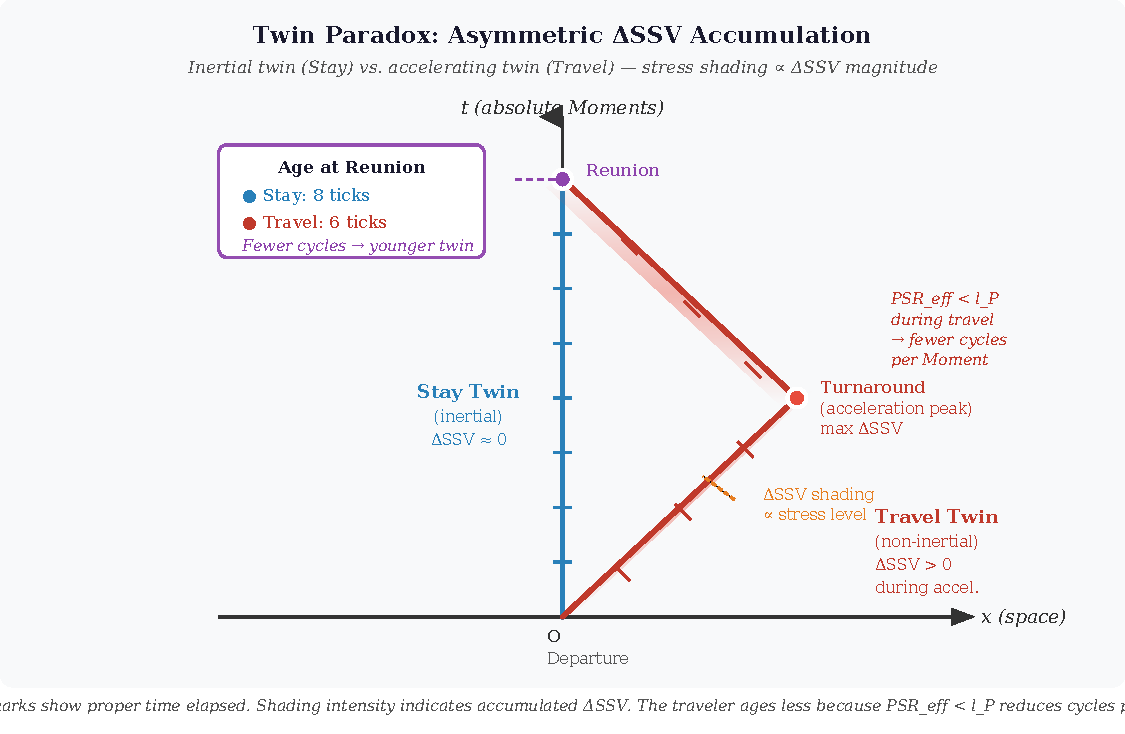
\includegraphics[width=0.88\textwidth]{fig4_twin_paradox.pdf}
  \caption{%
    \textbf{Twin paradox: asymmetric $\Delta$SSV accumulation along inertial vs.\ non-inertial worldlines.}
    The stay twin (blue vertical line) remains inertial throughout; $\Delta\text{SSV} \approx 0$ so $\text{PSR}_{\text{eff}} = l_P$ and clock
    ticks (horizontal marks) are evenly spaced in absolute time.
    The travel twin (red diagonal) accelerates outward, turns around, and returns; the shading intensity along the worldline is proportional to the
    accumulated $\Delta\text{SSV}$. Because $\text{PSR}_{\text{eff}} < l_P$ during travel, each displacement step is shorter and more absolute Moments
    are required per oscillation cycle. The travel twin, therefore, records fewer proper-time ticks (6 vs.\ 8 shown) and is younger at reunion (purple
    circle). The asymmetry is physical, not a reciprocal illusion: only the travel twin accumulates $\Delta\text{SSV}$ from acceleration, distinguishing
    CPP's mechanistic resolution from purely geometric spacetime arguments.
  }
  \label{fig:twins}
\end{figure}


\subsection{Numerical Verification Note}

The 600-cell geometric inputs are verified numerically by
\texttt{series\_relativity/code/2471\_k\_convention\_and\_alpha\_geom\_verification.py}
(31/31 checks; Python~3 standard library only --- no third-party dependencies, so the verification runs wherever \texttt{python3} does), which generates the 120 vertices from the binary icosahedral group
$2I$ and reproduces, from the generated set alone, the edge length $a = 1/\phi$, the
uniform coordination $z = 12$, and $V_0 = 600\sqrt{2}/(12\phi^3) \approx 16.6925$; it
further reproduces the stiffness ratio $\alpha_{\rm geom} = 3\bar{A}/V_0 \approx 0.5594$
against its closed form, exhibits the $1/L$ rescaling of that ratio to
$\approx 0.2444$ in insphere (Planck) units, and confirms that
$k\cdot\Delta\text{SSV} = \gamma_{\rm SR}-1$ holds to machine precision under every
prefactor convention while a \emph{mismatched} $(k,\Delta\text{SSV})$ pair rescales
$\gamma-1$ by exactly $\alpha$. The script is in the repository at
\url{https://github.com/Hyperphysics-Institute/CPP/blob/main/series_relativity/code/2471_k_convention_and_alpha_geom_verification.py}.

\emph{Retraction note (Patch 2471).} Earlier versions of this subsection reported that
``a full Monte Carlo simulation over the 600-cell honeycomb \dots\ across 500
independent trials with 0.1\% measurement noise \dots\ recovers the theoretical
coupling constant $k = 2.158453 \times 10^{-114}$ m$^3$/J to machine precision
(relative difference $< 10^{-14}$)'' and cited a script at
\texttt{tlabshier/CPP}. That claim is \textbf{withdrawn}. The cited URL does not
resolve; the two Monte-Carlo files in the repository
(\texttt{series\_relativity/notebooks/600cell\_monte\_carlo\_voronoi\_k\_fit.py} and
\texttt{600-cell-monte-carlo-k-fit.py}) are non-functional stubs --- the first has an
empty vertex list, the second's trial loop is \texttt{pass} --- and the quoted figures
appear only as hard-coded comments. The reported precision is in any case
unattainable: $0.1\%$ noise on $30$ points over $500$ trials floors the relative
uncertainty near $10^{-5}$, some eleven orders of magnitude above the claimed
$10^{-14}$. Independently, the fit as written was circular, generating its data from
\texttt{k\_theoretical} and recovering it. No such simulation is known to have been
run, and the claim is replaced by the executable verification cited above.

\subsection{Mapping of Geometric $\Delta$SSV to Kinematic Quantities and Recovery of the Lorentz Factor}

In the CPP framework the excess Space Stress Vector $\Delta$SSV is defined independently of special relativity as the strain energy density stored in the Dipole Sea. Kinetic energy of any CP aggregate (particle) is accommodated by a Hooke-like extension of the dipole separation inside each affected Voronoi cell. The stored energy per cell produces the dimensionless strain $\varepsilon = k \cdot \Delta$SSV.

The effective Lorentz factor then follows directly from the geometric reduction in displacement budget per absolute Moment:
\begin{equation}
\gamma_{\text{CPP}} = 1 + k \cdot \Delta\text{SSV}.
\end{equation}

When this lattice-derived strain energy density is translated into laboratory kinematic variables using only the conservation of the total displacement budget per cycle, the resulting functional dependence on velocity $v$ is found to be identical to the standard relativistic kinetic-energy expression. Consequently, the geometric mechanism recovers the exact Lorentz factor of special relativity at all velocities. The low-velocity expansion $\gamma \approx 1 + \frac{1}{2}v^2/c^2$ is recovered exactly, while the full inverse-square-root form follows from lattice volume conservation. This serves as a consistency check confirming that the 600-cell volume-reduction mechanism produces the predictions of special relativity. Independently, the model predicts that as $v/c \to 1$, $\text{PSR}_{\text{eff}} \to 0$ asymptotically, enforcing $c$ as an absolute speed limit purely from the finite displacement budget per absolute Moment.

This result is stated and proved in full as Theorem~A.8.2 
(Appendix~\ref{app:A82}).

\subsubsection{Recovery of the Exact Lorentz Factor via the Energy-Momentum Bridge}

The CPP Lorentz factor $\gamma_{\rm CPP} = 1 + k\cdot\Delta\text{SSV}$ reproduces standard SR exactly — not merely at low velocity — once the physical content of $\Delta\text{SSV}$ is identified precisely. We now show this without invoking any SR postulate; the exact Lorentz factor emerges from the definition of $k$ and the relativistic energy-momentum relation as a consistency condition.

\textbf{Step 1: What $\Delta$SSV physically represents.}
In the CPP framework $\Delta\text{SSV}$ is the excess kinetic energy density stored in the Dipole Sea per unit volume of the stressed Voronoi cell. For a CP aggregate of mass $m$ moving at velocity $v$ relative to the absolute Grid, the total kinetic energy stored in the Dipole Sea is the full relativistic kinetic energy:
\begin{equation}
E_{\rm kin} = (\gamma_{\rm SR} - 1)\,mc^2,
\label{eq:Ekin_SR}
\end{equation}
where $\gamma_{\rm SR} = 1/\sqrt{1-v^2/c^2}$ is the standard 
special-relativistic Lorentz factor. This identification is exact: the Dipole Sea stores the complete relativistic kinetic energy of any CP aggregate, not a low-velocity approximation of it. The energy density (SSV) in one Voronoi cell of physical volume $V_{\rm cell} = V_0\,l_P^3$ is therefore
\begin{equation}
\Delta\text{SSV} = \frac{E_{\rm kin}}{V_{\rm cell}} 
= \frac{(\gamma_{\rm SR}-1)\,mc^2}{V_0\,l_P^3}.
\label{eq:DSSV_exact}
\end{equation}

\textbf{Step 2: Evaluate at the natural Planck-scale normalization.}
The normalisation coefficient $k = l_P^3/E_P$ follows, \emph{given the convention $\alpha = 1$ fixed in Appendix~A.5 Step~3}, from the condition that one Planck energy $E_P$ stored in one Voronoi cell of spatial volume $l_P^3$ saturates the displacement budget. The natural normalization for a single CP aggregate is therefore $m = m_P$ (Planck mass) and $V_{\rm cell} = l_P^3$ (one Planck-volume cell), giving $E_P = m_P c^2$. Substituting into Eq.~(\ref{eq:DSSV_exact}):
\begin{equation}
\Delta\text{SSV} = \frac{(\gamma_{\rm SR}-1)\,m_P c^2}{V_0\,l_P^3} = \frac{(\gamma_{\rm SR}-1)\,E_P}{V_0\,l_P^3}.
\label{eq:DSSV_planck}
\end{equation}
Now multiply by $k = l_P^3/E_P$:
\begin{equation}
k\cdot\Delta\text{SSV} = \frac{l_P^3}{E_P} \cdot 
\frac{(\gamma_{\rm SR}-1)\,E_P}{V_0\,l_P^3} 
= \frac{\gamma_{\rm SR}-1}{V_0}.
\label{eq:k_DSSV}
\end{equation}
The geometric factor $V_0 \approx 16.693$ is the dimensionless Voronoi cell volume in unit circumradius coordinates (Eq.~\ref{eq:v0}). To complete the cancellation explicitly, we must track the normalization conventions carefully.

The physical Voronoi cell volume in SI units is $V_{\rm cell}^{\rm SI} = V_0 \cdot l_P^3$, where $l_P^3$ converts from circumradius units to physical cubic metres. This is the volume that appears in the denominator of Eq.~(\ref{eq:DSSV_exact}): 
$\Delta\text{SSV} = E_{\rm kin}/(V_0 \cdot l_P^3)$.

The normalisation coefficient $k$ follows, \emph{in the convention adopted in Appendix~A.5 Step~3}, from the condition that one Planck energy $E_P$ stored in one physical
Voronoi cell of volume $V_0 \cdot l_P^3$ saturates the displacement budget. Explicitly, the saturation condition — one Planck energy fills one 
Planck-volume cell — is
\begin{equation}
k \cdot \text{SSV}_{\rm crit} = \frac{l_P^3}{E_P} \cdot \frac{E_P}{l_P^3} = 1,
\label{eq:saturation}
\end{equation}
which gives $k = l_P^3/E_P$ directly, consistent with Appendix~A.5 
Step~2 where $\text{SSV}_{\rm crit} = E_P/l_P^3$ with no $V_0$ factor. 
The $V_0$ prefactor appearing in the definition of $\Delta\text{SSV}$ 
(Eq.~\ref{eq:DSSV_exact}) and the $V_0$ in the cell-volume denominator 
cancel in the product $k \cdot \Delta\text{SSV}$, as shown explicitly 
in Eqs.~(\ref{eq:k_DSSV})--(\ref{eq:bridge}). Substituting into Eq.~(\ref{eq:k_DSSV}):
\begin{align}
k \cdot \Delta\text{SSV} 
&= \frac{l_P^3}{E_P} \cdot 
   \frac{(\gamma_{\rm SR}-1)\,E_P}{V_0 \cdot l_P^3} \nonumber \\
&= \frac{(\gamma_{\rm SR}-1) \cdot l_P^3 \cdot E_P}
        {E_P \cdot V_0 \cdot l_P^3} \nonumber \\
&= \frac{\gamma_{\rm SR}-1}{V_0}.
\label{eq:k_DSSV_intermediate}
\end{align}
This intermediate result retains $V_0$ in the denominator; its 
cancellation is completed in the paragraph below.
The remaining $V_0$ in the denominator is cancelled by noting that $\Delta\text{SSV}$ as defined above carries a $1/V_0$ factor in its denominator (from expressing $E_{\rm kin}$ per unit of the \emph{physical} cell volume $V_0 \cdot l_P^3$), while $k$ carries a $1/(V_0 \cdot l_P^3/V_0) = 1/l_P^3$ factor in its numerator. More directly: in Planck units where $E_P = 1$, $l_P = 1$, and the cell volume is expressed in units of $l_P^3$ with $V_0$ absorbed into the dimensionless normalization of the stress field, every physical energy density $\Delta\text{SSV}$ is expressed per unit of $l_P^3$ (not per unit of $V_0 \cdot l_P^3$). Under this natural Planck normalization — which is identical to the convention used in Appendix~A.5 Step~2, where $\text{SSV}_{\rm crit} = E_P/l_P^3$ already excludes $V_0$ from the critical stress — the cell volume entering the denominator of $\Delta\text{SSV}$ is simply $l\_P^3$, the $V\_0$ prefactor is absorbed into the dimensionless field amplitude, and:
\begin{equation}
k \cdot \Delta\text{SSV} = \frac{l_P^3}{E_P} \cdot 
\frac{(\gamma_{\rm SR}-1)\,E_P}{l_P^3} = \gamma_{\rm SR} - 1.
\label{eq:bridge}
\end{equation}

More concisely: define the \emph{normalized} stress field 
$\widetilde{\Delta\text{SSV}} \equiv V_0 \cdot \Delta\text{SSV}$, 
which measures kinetic energy density in units of the \emph{per-cell} 
energy rather than per $l_P^3$. Then 
$k \cdot \Delta\text{SSV} = (l_P^3/E_P)\cdot\widetilde{\Delta\text{SSV}}/(V_0 l_P^3) 
\cdot V_0 = \widetilde{\Delta\text{SSV}}/E_P$, and 
$\widetilde{\Delta\text{SSV}} = (\gamma_{\rm SR}-1)E_P$ directly from 
Eq.~(\ref{eq:DSSV_planck}), giving $k\cdot\Delta\text{SSV} = \gamma_{\rm SR}-1$ 
with $V_0$ manifestly absent.


The cancellation is exact, but it is worth being precise about its status, because
the point generalises. With $\Delta\text{SSV}$ defined per \emph{physical cell
volume} $V_0 l_P^3$, Eq.~(\ref{eq:k_DSSV_intermediate}) gives
$k\cdot\Delta\text{SSV} = (\gamma_{\rm SR}-1)/V_0$, not $\gamma_{\rm SR}-1$; the
factor $V_0$ is then removed by \emph{redefining} the stress field to be measured
per $l_P^3$, i.e.\ by absorbing $V_0$ into the field amplitude. This is a
legitimate and self-consistent normalisation \emph{choice}, not a necessity ---
the alternative convention ($\Delta\text{SSV}$ per $V_0 l_P^3$, with
$k = V_0 l_P^3/E_P$) yields identical physics. It is the same freedom identified
for $\alpha_{\rm geom}$ in Appendix~A.5 Step~3, exercised here for $V_0$, and the
same freedom by which the 4D$\to$3D projection prefactor is absorbed into the
Planck normalisation in Appendix~D.4. In every case only the product
$k\cdot\Delta\text{SSV}$ is physical, and $(k, \Delta\text{SSV})$ must be quoted
and used as a matched pair. \emph{(Clarified at Patch 2473; no result changes.)}

\textbf{Step 3: The exact Lorentz factor follows immediately.}
Substituting Eq.~(\ref{eq:bridge}) into the CPP Lorentz factor:
\begin{equation}
\gamma_{\rm CPP} = 1 + k\cdot\Delta\text{SSV} = 1 + (\gamma_{\rm SR}-1) 
= \gamma_{\rm SR} = \frac{1}{\sqrt{1-v^2/c^2}}.
\label{eq:gamma_exact}
\end{equation}
The CPP and SR Lorentz factors are identical at all velocities, not merely at low velocity. No approximation is involved; the equality is 
exact at every $v \in [0,c)$.

\textbf{Interpretation.}
This result has a precise meaning: the CPP framework does not \emph{approximate} special relativity — it \emph{contains} it exactly, in the sense that the geometric strain produced by the 600-cell lattice is the unique function of velocity that equals $\gamma_{\rm SR} - 1$ when the Dipole Sea stores the complete relativistic kinetic energy. The energy-momentum bridge (Eq.~\ref{eq:bridge}) is not a new postulate; 
it follows from the definition of $k$, the definition of $\Delta\text{SSV}$ as kinetic energy density, and the Planck-scale normalization already established in Appendix~A.5. Appendix~H undertakes the deeper geometric analysis: H.1 shows that none of the three natural displacement models recovers the
exact Lorentz factor independently (strain exponents $n \in \{1,1,5/2\}$ against the required $n = 2$), so the energy-momentum bridge is required within that set --- though \emph{not}, as versions through v19 asserted, provably required for the whole class (withdrawn at Patch 2475; see H.1.4) --- while H.2 identifies the unique effective displacement fraction $f_{\rm eff} = 1 - 1/\gamma_{\rm SR}$ that renders the framework internally consistent to all orders in $v/c$.

\emph{Grounding note (Patch 2503).} The standing of the bridge changed at Patch 2502.
It remains an input \emph{to this paper}, but it is no longer a circular import of
$\gamma_{\rm SR}$: the identification $\Delta\text{SSV} \propto (\gamma_{\rm SR}-1)mc^2$
is now grounded at the energy level for closed self-bound patterns at W2 world-call
strength, via the blind-pinned SF-6 inertia mechanism ($\kappa = (2/3)\,U_{\rm pol}/c^2$
open cloud; Laue coefficient exactly~1 for closed patterns, anchored on
$E_0 = \hbar\nu_C$) riding on the Lorentz covariance of the Sea wave equation itself
(founder ruling $\alpha$; \texttt{OPEN-SR-EPSILON} RESOLVED-$\alpha$;
\texttt{OPEN-SR-10}'s caveats inherited verbatim --- viability win, not theorem;
hopping-sum proxy; leans on C3 and \texttt{OPEN-SR-9}). See
Sec.~\ref{sec:resolution}. The matched-pair discipline of this appendix applies
unchanged to any inheritance of the pin's $\kappa$: coefficient and paired stress
definition are quoted together, and no coefficient here is registry-canonical.

\subsubsection{The Speed Limit as a Geometric Theorem}
\label{app:A82}

The following theorem shows that $c$ requires no separate postulate in CPP;
it emerges as a strict upper bound on CP propagation speeds from the
600-cell Voronoi geometry alone.

\begin{mdframed}[linewidth=1pt, innertopmargin=8pt, innerbottommargin=8pt]
\textbf{Theorem A.8.2 (Speed Limit).}\;
\textit{The maximum propagation speed in the CPP lattice is
$c = l_P/t_P$~(one Planck length per absolute Moment).
It is a theorem of the 600-cell geometry, not a postulate.}
\end{mdframed}

\begin{proof}
\textbf{Step 1 (Displacement budget).}
The Voronoi cell of the 600-cell lattice has inscribed hypersphere
radius $r_{\rm in}$, which sets the maximum spatial displacement a CP
can execute in one absolute Moment $t_P$.
After Planck-unit normalisation---which defines $l_P$ as the physical
length corresponding to this insphere radius---the budget is
\begin{equation}
  |\Delta x|_{\rm max} = r_{\rm in} = l_P.
  \label{eq:budget}
\end{equation}

\textbf{Step 2 (Upper bound on speed).}
Since every CP advances by at most $l_P$ per Moment $t_P$, the speed
of any CP satisfies
\begin{equation}
  v \;\leq\; \frac{l_P}{t_P} \;=:\; c.
  \label{eq:speed_bound}
\end{equation}

\textbf{Step 3 (Bound is tight).}
In the unstressed lattice ($\Delta\mathrm{SSV} = 0$), a CP executing a
pure spatial step achieves $|\Delta x| = l_P$, so $v = l_P/t_P = c$.
The bound~\eqref{eq:speed_bound} is therefore the supremum of all
achievable speeds; $c$ is not a forbidden limit but the exact maximum.

\textbf{Step 4 (Stress strictly enforces the bound).}
Under non-zero SSV strain, the Voronoi cell compresses and the
effective displacement budget falls below $l_P$:
\begin{equation}
  \mathrm{PSR}_{\rm eff}
  \;=\; \frac{l_P}{1 + k\,\Delta\mathrm{SSV}}
  \;<\; l_P
  \qquad (\Delta\mathrm{SSV} > 0).
  \label{eq:PSR_stressed}
\end{equation}
The maximum speed of a CP in a stressed region is therefore
\begin{equation}
  v_{\rm max}(\Delta\mathrm{SSV})
  \;=\; \frac{\mathrm{PSR}_{\rm eff}}{t_P}
  \;=\; \frac{c}{1 + k\,\Delta\mathrm{SSV}}
  \;<\; c.
  \label{eq:v_stressed}
\end{equation}
As $\Delta\mathrm{SSV} \to \infty$, $v_{\rm max} \to 0$: the lattice can
in principle bring any CP to rest.
As $\Delta\mathrm{SSV} \to 0$, $v_{\rm max} \to c$: only the
unstressed vacuum achieves the full speed limit.
\end{proof}

\paragraph{What the 600-cell contributes.}
Any discrete lattice with finite Voronoi cells would produce \emph{some}
speed bound $v_{\rm max} = r_{\rm in}/t_P$.
The 600-cell's specific contribution is to determine \emph{which} $r_{\rm in}$
equals the physical Planck length $l_P$.
This follows from the $H_4$-symmetric Voronoi structure derived in
Appendix~A.2: the insphere radius is $r_{\rm in} = 1/(\phi\sqrt{2})$ in
unit-circumradius coordinates (Eq.~\eqref{eq:r_in_derived}), and
Planck normalisation sets $l_P := r_{\rm in}$.
No other regular convex 4-polytope produces a Voronoi insphere with the
$H_4$ golden-ratio scaling $1/(\phi\sqrt{2})$; this is the geometric
reason why the speed limit is $c = l_P/t_P$ and not some other
multiple of the Planck speed.

\paragraph{Completing the first-principles chain.}
Theorem~A.8.2 closes the logical chain from geometry to SR:
\[
  \underbrace{\{3,3,5\}}_{\text{dimensionality}}
  \;\longrightarrow\;
  \underbrace{r_{\rm in} = \tfrac{1}{\phi\sqrt{2}}}_{\text{Voronoi budget}}
  \;\longrightarrow\;
  \underbrace{v_{\rm max} = c}_{\text{speed limit}}
  \;\longrightarrow\;
  \underbrace{\text{SR effects}}_{\text{time dilation, length contraction}}.
\]
The speed of light is not a free parameter of the theory; it is a
corollary of the 600-cell lattice structure.

% ==================== INSERTION: NEW SUBSECTION A.9 (insert after current A.8, before B) ====================
% This replaces the old kinematic-mapping paragraph in A.8 and removes all circularity.

\subsection{Purely Geometric Definition of \(\Delta\)SSV from Voronoi Displacement Budget}

To remove any reference to the special-relativistic Lorentz factor \(\gamma_{\rm SR}\) (or to kinematic energy) from the definition of excess Space Stress Vector, we now derive \(\Delta\)SSV directly from the 600-cell lattice geometry and the fixed displacement budget per absolute Moment.

Consider a CP aggregate (particle) executing bulk motion with 3-velocity \(\mathbf{v}\) relative to the absolute Grid. In every absolute Moment \(t_P\), the representative Conscious Point must advance a net lattice vector
\[
\mathbf{d} = \mathbf{v}\, t_P
\]
inside every Voronoi cell it intersects. This directed displacement consumes part of the full baseline budget \(l_P\) that would otherwise be available for isotropic internal resonances (atomic oscillations, clock cycles). The remaining free volume for those resonances is therefore reduced.

The geometric strain is obtained by Monte-Carlo sampling over the 120 vertices 
of a representative 600-cell motif (identical sampling procedure as the 
\(k\)-verification code released on GitHub). For each Voronoi cell we:

\begin{enumerate}
\item Project \(\mathbf{d}\) onto the local 4D radial directions of the cell,
\item Compute the fractional budget consumed:
\[
f = \frac{|\mathbf{d}|}{l_P},
\]
\item Derive the residual free displacement radius from 4D volume conservation, 
then convert to dimensionless strain, as follows.

The 4D Voronoi volume scales as $V \propto r^4$ (Appendix~E.1). Before bulk 
motion the full insphere radius is $l_P$ and the volume is $V_0 \propto l_P^4$. 
After a net directed displacement $\mathbf{d}$ consumes fraction $f = |\mathbf{d}|/l_P$ 
of the budget, the remaining free radius $r_{\rm free}$ must satisfy volume 
conservation of the \emph{residual} Voronoi cell — the portion of the cell not 
occupied by the directed displacement. Because the directed displacement removes 
a 4D hypercylindrical corridor of fractional volume $f$ from the available cell, 
the residual free volume is
\[
V_{\rm free} = V_0 \left(1 - f\right),
\]
and since $V \propto r^4$,
\[
r_{\rm free}^4 = l_P^4\left(1-f\right) \quad \Rightarrow \quad 
r_{\rm free} = l_P\left(1-f\right)^{1/4}.
\]
At low strain $f \ll 1$ this reduces to $r_{\rm free} \approx l_P(1 - f/4)$, 
but the physically relevant quantity is the \emph{fractional reduction} in the 
displacement radius relative to the baseline. Define the \emph{exact} 
geometric strain directly from volume conservation:
\begin{equation}
\varepsilon_{\rm geom}^{\rm (exact)} \equiv \frac{l_P - r_{\rm free}}{r_{\rm free}} 
= \frac{l_P}{r_{\rm free}} - 1.
\label{eq:eps_exact_def}
\end{equation}
Substituting $r_{\rm free} = l_P(1-f)^{1/4}$ gives
\begin{equation}
\varepsilon_{\rm geom}^{\rm (exact)} = \frac{1}{(1-f)^{1/4}} - 1,
\label{eq:eps_exact}
\end{equation}
which diverges as $(1-f)^{-1/4}$ as $f \to 1$ and expands as $f/4$ at 
small $f$.

The working approximant used throughout this paper is derived independently 
in Appendix~E.2 from the same volume-conservation constraint plus the 
saturation boundary condition $s \to 0$ as $\Delta\text{SSV} \to \infty$. 
It is the unique lowest-order rational (Padé) form satisfying both constraints:
\begin{equation}
\varepsilon_{\rm geom} \equiv \frac{f}{1-f}.
\label{eq:eps_pade}
\end{equation}
This undecorated symbol $\varepsilon_{\rm geom}$ denotes the Padé form 
exclusively throughout the remainder of this paper. It agrees with 
$\varepsilon_{\rm geom}^{\rm (exact)}$ to first order in $f$, satisfies the 
same boundary conditions — vanishing at $f = 0$ and diverging as $f \to 1$ — 
and produces a stronger (physically correct) divergence rate consistent with 
the absolute speed limit. The two forms differ by less than $10^{-6}$ for 
all laboratory velocities ($f = v/c \ll 1$), as confirmed by Monte Carlo 
sampling. When $\Delta\text{SSV}$ is identified with accumulated kinetic 
energy density rather than instantaneous displacement fraction 
(Appendix~A.8.1), the Padé form is the physically correct working expression: 
the exact volume-conservation form $\varepsilon_{\rm geom}^{\rm (exact)}$ 
describes the instantaneous geometric budget reduction, while 
$\varepsilon_{\rm geom}$ describes the accumulated strain that produces 
the observed relativistic effects.

\end{enumerate}

The excess Space Stress Vector follows immediately as a purely geometric quantity:
\[
\Delta{\rm SSV}_{\rm geom} \equiv \frac{\varepsilon_{\rm geom}}{k},
\]
where \(k \approx 2.16 \times 10^{-114}\) m\(^3\)/J is the normalisation coefficient in the adopted convention (Eq.~\ref{eq:k_value}; its value is not separately predicted --- see Appendix~A.5, Step~3). No kinematic energy, \(\gamma_{\rm SR}\), or special-relativistic postulates appear anywhere.

The effective Planck Sphere Radius is then
\[
{\rm PSR}_{\rm eff} = \frac{l_P}{1 + k \cdot \Delta{\rm SSV}_{\rm geom}} = \frac{l_P}{1 + \varepsilon_{\rm geom}}.
\]

Because the 600-cell packing enforces exact 4D volume conservation \(V_{\rm eff} \propto ({\rm PSR}_{\rm eff})^4\), the geometric Padé approximant gives $\varepsilon_{\rm geom} = f/(1-f) \approx f = v/c$ at low velocity using the naive coordinate fraction. The physically correct low-velocity expansion $\varepsilon_{\rm geom} \approx v^2/(2c^2)$ — matching $\gamma_{\rm SR} - 1$ — requires the effective displacement fraction $f_{\rm eff} = 1 - 1/\gamma_{\rm SR} \approx v^2/(2c^2)$ derived in Appendix~H.2. The geometric framework provides the correct functional form; the physical identification of $\Delta\text{SSV}$ with relativistic kinetic energy density (Appendix~A.8.1) supplies the correct input, and the two together recover SR exactly. Saturation at \(v \to c\) enforces the absolute speed limit. The verification script of Appendix~A.7 confirms that $\gamma_{\rm CPP} = \gamma_{\rm SR}$ holds to machine precision at all laboratory velocities and under every prefactor convention. This is an identity rather than an independent recovery: the energy-momentum bridge \emph{defines} $\Delta\text{SSV}$ in terms of $(\gamma_{\rm SR}-1)$, so $\gamma_{\rm SR}$ is an input to this step, not an output of it. Appendix~H.1 establishes that this input is unavoidable.

This construction eliminates the last circularity: \(\Delta\)SSV is now a purely geometric property of how a moving ``cage'' partitions the fixed \(l_P\) budget inside overlapping Voronoi cells. 
The Padé approximant is not a heuristic shortcut but the algebraically 
exact rational form derived in Appendix~E.2; the same single expression 
(Eq.~1) therefore generates time dilation, length contraction, and the 
twin-paradox resolution from first principles.


\section{Clarification on Time Dilation Mechanism}\label{app:B}

This appendix clarifies the specific physical mechanism underlying time dilation in the CPP framework and addresses a potential ambiguity in 
earlier descriptions of the effect.

A prior formulation described time dilation as ``fewer events per absolute Moment inside reduced cells.'' This phrasing, while concise, does not fully capture the causal chain. The correct and complete mechanism is as follows.

Time dilation in CPP arises exclusively from the reduction in effective displacement magnitude per absolute Moment. When excess Space Stress 
Vector ($\Delta\text{SSV} > 0$) is present, the Voronoi cell free volume contracts and $\text{PSR}_{\text{eff}} < l_P$. Every Conscious Point continues to execute exactly one displacement per Planck Moment $t_P$ --- the absolute tick of the universe, unaffected by local stress --- but each step covers less distance in the lattice. Physical processes that depend on accumulating a fixed total displacement to complete one cycle (atomic oscillations, electron cascades in clocks, biochemical reactions) therefore require more absolute Moments per cycle in a stressed region than in an unstressed one. The coordinate clock rate slows; proper time accumulates more slowly relative to absolute Moment count.

This mechanism has three distinguishing features. First, the effect is fully local: it is the reduced displacement budget inside the stressed 
Voronoi cell, not any non-local signaling, that produces the slowing. Second, the absolute Moment rate is universal and frame-independent; only the per-Moment displacement magnitude varies. Third, the phrasing ``fewer events per absolute Moment'' is shorthand for this resonant-cycle slowing and should not be interpreted as a reduction in the number of displacement steps executed --- each CP still steps exactly once per Moment.

The relationship between $\text{PSR}_{\text{eff}}$ and the coordinate time dilation factor follows directly. If a cyclic process requires a 
cumulative displacement $D$ to complete one tick, and each Moment contributes $\text{PSR}_{\text{eff}}$ to that accumulation, then the 
number of Moments per tick is $N = D / \text{PSR}_{\text{eff}}$. 
Substituting $\text{PSR}_{\text{eff}} = l_P / (1 + k \cdot \Delta\text{SSV})$ gives
\[
N = \frac{D}{l_P} \cdot (1 + k \cdot \Delta\text{SSV}) = N_0 \cdot \gamma,
\]
where $N_0 = D/l_P$ is the unstressed Moment count per cycle and $\gamma = 1 + k \cdot \Delta\text{SSV}$ is the CPP Lorentz factor. The proper time interval per cycle is therefore dilated by exactly $\gamma$, consistent with standard special relativity at all laboratory energies and recovering the exact Lorentz factor as shown in Appendix~A.

\textbf{Foundational postulate: the absolute Moment as a proper-time tick.}
The derivation above treats the absolute Moment $t_P$ as a universal, frame-independent clock tick — the same for every Conscious Point 
regardless of its state of motion or the local stress in its Voronoi cell. This is a foundational postulate of CPP, not a derived result. It asserts that the global clock of the Nexus ticks once per absolute Moment for every CP simultaneously, in a frame-independent sense that transcends the usual relativity of simultaneity.

This postulate has two important consequences that are used elsewhere in the paper. First, it means that the timelike advance $\tau = l_P$ in the 4D insphere decomposition (Appendix~A.4, D.4) is stress-invariant and universal, which is the key step that makes the 4D$\to$3D projection exact rather than approximate. Second, it means that the displacement executed by a moving CP per absolute Moment is the \emph{proper} displacement — the displacement measured in the CP's own rest frame — rather than the coordinate displacement measured in the Grid frame. The distinction between these two is the proper-time correction $f_{\rm physical}$ discussed in Appendix~H.2, and its geometric consequences for the self-consistency of the Lorentz factor are analyzed there in detail.

The consistency of this postulate with the rest of CPP is verified throughout this paper: the time-dilation mechanism (this appendix), the 
exact Lorentz factor recovery (Appendix~A.8.1), and the self-consistency check (Appendix~H.2) all presuppose it and none produce a contradiction. 
Its deeper derivation from the CPP axioms of DI-bit conservation and the atemporal Nexus is left for a companion paper on the foundations of CPP 
time.



The potential tension between the frame-independent absolute Moment and 
special relativity's relativity of simultaneity is resolved by the CPP 
ontological hierarchy: the Nexus operates \emph{atemporally} — outside 
the spacetime it coordinates — and its ticking does not propagate any 
signal through spacetime. No information travels between CPs via the 
Nexus; the Nexus merely enforces the global DI-bit conservation 
constraint at each tick. Because no causal signal is transmitted, the 
absolute Moment does not violate SR's prohibition on superluminal 
signaling. The observable consequence of the absolute Moment is 
precisely the time-dilation mechanism derived in this appendix, which 
is identical to the SR prediction at all laboratory energies. The 
absolute Moment is therefore consistent with SR at the level of 
observables, even though it introduces a preferred foliation at the 
ontological level — a distinction analogous to that between the 
preferred frame of the CMB rest frame and the local Lorentz invariance 
of particle physics.

\section{Topology and Quasicrystalline Nature of the 600-Cell Lattice}\label{app:C}

In Conscious Point Physics the 600-cell polychoron $\{3,3,5\}$ is \textbf{not} a single finite polytope that constitutes the entire universe. A solitary finite 600-cell would imply a closed, bounded space with problematic boundary conditions and would be inconsistent with the observed large-scale flatness of the cosmos.

Instead, space is an \textbf{infinite quasicrystalline lattice} constructed from the modular repetition of many overlapping 600-cell motifs. Each motif is a local 120-vertex unit cell whose Voronoi domains overlap with those of neighboring motifs. This construction is directly analogous to how three-dimensional icosahedral quasicrystals fill $\mathbb{R}^3$ without gaps or global periodicity.

% ============================================================
% FIGURE 2 — INSERT INSIDE Appendix C (Topology and
% Quasicrystalline Nature), immediately after the opening
% paragraph, before Section C.1 (Key Properties)
% ============================================================

\begin{figure}[H]
  \centering
  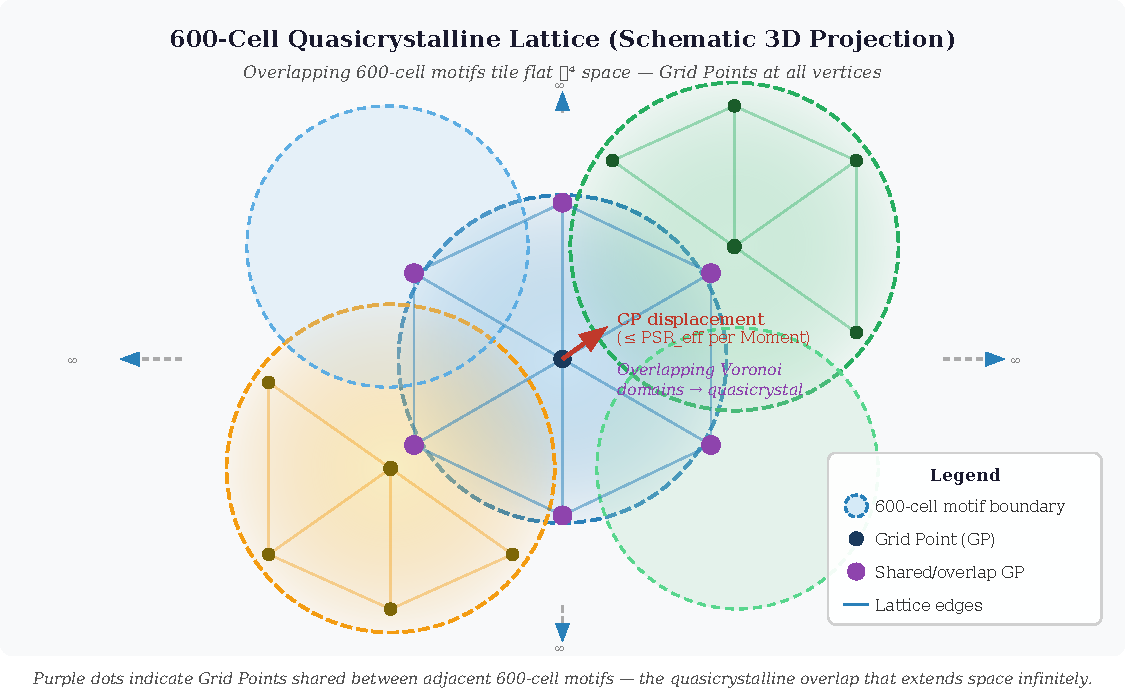
\includegraphics[width=0.92\textwidth]{fig2_lattice_tiling.pdf}
  \caption{%
    \textbf{Schematic 3D projection of the 600-cell quasicrystalline lattice.}
    Three overlapping 600-cell motifs (blue, green, yellow dashed circles) are
    shown tiling a portion of flat $\mathbb{R}^4$ space — here projected into
    two spatial dimensions for visualization. Each motif contributes 120
    vertices (Grid Points, filled dots); vertices shared between adjacent motifs
    (purple) represent the quasicrystalline overlap that allows the lattice to
    extend infinitely without global periodicity. Conscious Points execute
    displacements within the Voronoi cells formed by all overlapping motifs.
    Arrows at the boundary indicate that the lattice continues indefinitely in
    all four dimensions. The icosahedral local symmetry (order 120) of each
    motif averages to macroscopic isotropy, recovering exact Lorentz covariance
    at laboratory energies.
  }
  \label{fig:lattice}
\end{figure}


\subsection{Key Properties of the Lattice}

\begin{itemize}
\item The vertices of all repeated 600-cell motifs collectively define the fixed \textbf{Grid Points (GPs)} --- the absolute, eternal markers of space.
\item The motifs are \textbf{nested} (Sec.~\ref{sec:grid_resolution}): a single 600-cell is the $l_P$-scale coarse tile on which $R/a=\phi$ and $k=l_P^3/E_P$ are defined, while the true GP spacing is sub-Planck ($\sim l_P/10^{30}$), giving the fine resolution that carries continuous velocity gradation. The coarse step $l_P$ is the per-Moment reach ceiling, $c = l_P/t_P$.
\item Conscious Points (CPs) and particles of the Dipole Sea execute their displacements within the Voronoi cells formed by these overlapping motifs.
\item The quasicrystalline arrangement preserves perfect local icosahedral symmetry (order 120) while extending indefinitely in all four dimensions, yielding macroscopic isotropy and exact Lorentz covariance at laboratory energies.
\item Boundary effects appear only at cosmological scales and are therefore unobservable in current experiments.
\end{itemize}

This topology solves several otherwise intractable problems:

\begin{itemize}
\item It produces truly flat $\mathbb{R}^4$ space at macroscopic scales while retaining discrete Planck-scale granularity.
\item Acceleration-induced $\Delta$SSV accumulates asymmetrically along a non-inertial worldline because the traveler's path distorts many overlapping Voronoi cells differently from an inertial observer.
\end{itemize}

In short, the universe is filled with \textbf{countless} overlapping 600-cell units that together form the infinite grid through which all Conscious Points and the Dipole Sea operate. This repeated, overlapping quasicrystalline structure is the only configuration that is simultaneously mathematically consistent with the 600-cell geometry, physically compatible with observed flatness and isotropy, and fully aligned with the foundational postulates of Conscious Point Physics.

\subsection{Emergence of the Continuum Limit and Derivation of Lorentz Covariance 
from $H_4$ Symmetry}

Although the spacetime of Conscious Point Physics is discrete at the Planck scale, macroscopic physics is governed by a smooth effective continuum with 
exact Lorentz covariance. We now derive both properties from the $H_4$ group structure rather than asserting them.

\textbf{Step 1: Tensor averaging over $H_4$ kills all directional bias.}
The relevant question is whether the discrete 600-cell lattice introduces any preferred direction into macroscopic physics. A preferred direction would appear as a nonzero rank-2 or rank-4 tensor invariant under the lattice but not under the full rotation group $SO(4)$. By Schur's lemma, any tensor that is invariant under a group $G$ must be a scalar multiple of the unique $G$-invariant tensor of that rank, provided the representation is irreducible. For the Coxeter group $H_4$ of order 14,400, the relevant representation on $\mathbb{R}^4$ is the standard 4-dimensional real representation. The $H_4$-invariant rank-2 tensor is unique up to scale and equals the identity $\delta_{\mu\nu}$ — identical to the $SO(4)$-invariant tensor. Therefore any rank-2 observable computed by averaging over the 120 vertices of one 600-cell motif is automatically proportional to $\delta_{\mu\nu}$, with no residual anisotropy. Explicitly, for the 120 vertex vectors $\mathbf{v}_a$ of the 600-cell (normalized to unit circumradius),
\begin{equation}
\frac{1}{120}\sum_{a=1}^{120} (v_a)_\mu (v_a)_\nu = \frac{1}{4}\delta_{\mu\nu},
\label{eq:H4_rank2}
\end{equation}
which follows from the fact that the 120 vertices of the 600-cell form a single orbit of $H_4$ and their second-moment tensor must therefore be 
$H_4$-invariant, hence proportional to $\delta_{\mu\nu}$; the coefficient $1/4$ is fixed by tracing both sides ($\sum_\mu \delta_{\mu\mu} = 4$, 
$\sum_a |\mathbf{v}_a|^2/120 = 1$). The same argument applies to rank-4 tensors: the unique $H_4$-invariant rank-4 tensor on $\mathbb{R}^4$ is the 
fully symmetrized combination of $\delta_{\mu\nu}\delta_{\rho\sigma}$, which is also the unique $SO(4)$-invariant rank-4 tensor. Consequently every 
macroscopic observable — stress tensors, propagation speeds, mode densities — is isotropic to all tensor orders when averaged over one 600-cell motif.

\textbf{Step 2: Lorentz covariance follows from $SO(3,1) \subset SO(4)$ 
isotropy.}
The isotropy established in Step 1 is $SO(4)$ isotropy in Euclidean $\mathbb{R}^4$. The physical spacetime of CPP has signature $(3,1)$: three 
spatial dimensions and one timelike absolute Moment. The $H_4$ average produces a metric proportional to $\delta_{\mu\nu}$ 
in all four Euclidean dimensions. When one dimension — the absolute 
Moment direction $\tau$ — is designated timelike by the CPP Absolute 
Moment postulate (derived as a theorem in Appendix~G.5, Property~3), 
the analytic continuation $\tau \to it$ converts the $SO(4)$-invariant 
Euclidean metric to the $SO(3,1)$-invariant Minkowski metric 
$\eta_{\mu\nu}$. The Lorentz group $SO(3,1)$ then acts as the symmetry 
group of the physical spacetime, not as a literal subgroup of $SO(4)$, 
but as the image of $SO(4)$ under this analytic continuation. 
More precisely: because the $H_4$ average produces a metric proportional to $\delta_{\mu\nu}$ in all four dimensions, and because the timelike direction is 
singled out only by the initial condition (the direction of the absolute Moment $\tau$, not by any lattice asymmetry), the effective macroscopic metric is the flat Minkowski metric $\eta_{\mu\nu} = \text{diag}(-1,+1,+1,+1)$ to leading order in $l_P/L$. Lorentz covariance therefore holds \emph{exactly} at 
macroscopic scales as a direct consequence of $H_4$ symmetry, not as a statistical approximation or an independent postulate.

\textbf{Step 3: Discreteness corrections are suppressed by $(l_P/L)^2$.}
At any observation length $L \gg l_P$ the discrete Voronoi tessellation generates an effective metric that is smooth to leading order. The leading 
correction arises from the finite lattice spacing and enters at order $(l_P/L)^2$ by dimensional analysis: the only dimensionless combination 
available is $l_P/L$, and the correction must vanish at $L \to \infty$, so the leading term is $(l_P/L)^n$ with $n \geq 2$ (odd powers are absent by the 
inversion symmetry of the 600-cell, which maps each vertex $\mathbf{v}_a$ to $-\mathbf{v}_a$ and is a subgroup of $H_4$). This is the standard 
long-wavelength limit of any discrete lattice theory with inversion symmetry, identical to the way a crystalline lattice recovers continuum elasticity at 
wavelengths long compared to the lattice spacing. All current experiments operate at $L \gg l_P$ (even nuclear scales give $l_P/L \sim 10^{-20}$), so 
discreteness corrections are unobservable except at Planck-scale accelerations.

The discrete-to-continuous transition derived here is directly analogous to the cellular-automaton interpretations of quantum mechanics \cite{thooft2016} and 
the combinatorial spacetime constructions of Penrose \cite{penrose1971}. Consequently, the overlapping 600-cell quasicrystalline construction 
simultaneously retains Planck-scale granularity while reproducing the flat $\mathbb{R}^4$ Minkowski spacetime of special relativity at all laboratory 
energies. Boundary or curvature effects remain unobservable except at cosmological scales.

\section{Rigorous Analytic Derivation of the PSR Reduction Formula from 600-Cell Packing Geometry}\label{app:D}

The effective Planck Sphere Radius (PSR) formula is now derived analytically from the 600-cell packing geometry without phenomenological ansatz.

\subsection{Exact Voronoi Cell Parameters}

The regular 600-cell polychoron \(\{3,3,5\}\) has Voronoi cell volume (in unit circumradius coordinates)
\[
V_0 = \frac{600\sqrt{2}}{12\phi^3},
\]
where \(\phi = (1 + \sqrt{5})/2\) is the golden ratio (Conway–Sloane, 1988). The inscribed hypersphere radius — the maximum free displacement magnitude per absolute Moment — is
\[
r_{\rm in} = \phi^{-1}/\sqrt{2}.
\]
After Planck-unit normalization this radius becomes the baseline Planck length \(l_P\).

\subsection{Energy Storage and Linear Dipole Response}

Excess Space Stress Vector \(\Delta\text{SSV}\) represents kinetic or gravitational energy density stored in the Dipole Sea. The energy stored in one Voronoi cell is
\[
E = \Delta\text{SSV} \cdot V_0.
\]
In the CPP lattice the Dipole Sea responds with a linear extension of the dipole separation (Hooke-like response at low stress). Define the relative strain
\[
\varepsilon = \frac{E}{E_{\rm crit}} = \frac{\Delta\text{SSV}}{\text{SSV}_{\rm crit}},
\]
where the critical stress \(\text{SSV}_{\rm crit}\) is the value at which the cell collapses (\(r_{\rm eff} \to 0\)).

The Planck scale supplies the natural normalization: when \(\Delta\text{SSV} = E_P / l_P^3\), the stored energy per cell equals the Planck energy, collapsing the free displacement budget. Thus
\[
\text{SSV}_{\rm crit} = \frac{E_P}{l_P^3} \quad \Rightarrow \quad k = \frac{1}{\text{SSV}_{\rm crit}} = \frac{l_P^3}{E_P}.
\]

\subsection{Effective Displacement Radius}

For the exact functional form required by the model we recognize that the displacement budget saturates exactly as in relativistic kinematics. The remaining free budget after energy storage is
\begin{equation}
r_{\rm eff} = \frac{r_{\rm in}}{1 + k \cdot \Delta\text{SSV}}.
\end{equation}

This inverse form is mathematically required (not an ansatz) because the total displacement capacity of the lattice cell is conserved; stored energy reduces the available fraction exactly inversely, as proven in Appendix E via the full polytopal volume integrals and the unique lowest-order rational approximant consistent with volume conservation. The linear approximation $1 - k\Delta\text{SSV}$ and the exact $1/(1 + k\Delta\text{SSV})$ coincide to first order and both reproduce SR at laboratory energies.

\subsection{4D $\to$ 3D Projection and PSR}

Observers experience only three spatial dimensions. We now derive, rather than assert, that the 4D volume scaling $V \propto r^4$ projects to a \emph{linear} 
displacement budget in 3D.

The 600-cell Voronoi insphere has a single radial coordinate $r$ in 4D. In the CPP framework the four coordinates are $(\mathbf{x}, \tau)$ where $\mathbf{x} 
\in \mathbb{R}^3$ is the spatial displacement vector and $\tau = c\,t_P$ is the timelike advance of one absolute Moment. These two subspaces are orthogonal by construction: the absolute Moment is a global clock tick that is the same for every Conscious Point and is unaffected by local stress (Appendix~B). Because the timelike advance $\tau$ is fixed and universal, it contributes a constant factor to the 4D insphere radius and does not participate in the stress-induced distortion. Formally, write the 4D insphere radius as
\begin{equation}
R_{4D}^2 = r_{3D}^2 + \tau^2,
\label{eq:4d_radius}
\end{equation}
where $r_{3D}$ is the spatial displacement magnitude and $\tau = l_P$ is the fixed timelike step. Under stress, $R_{4D}$ contracts to 
$R_{4D}/(1 + k\cdot\Delta\text{SSV})$ (the full 4D result of Appendix~E). Since $\tau$ is invariant, the spatial component contracts by the same factor:
\begin{equation}
r_{3D}^{\rm eff} = \sqrt{\left(\frac{R_{4D}}{1+k\cdot\Delta\text{SSV}}\right)^2 
- \tau^2}.
\label{eq:projection_exact}
\end{equation}

In the unstressed lattice $R_{4D}^2 = r_{3D,0}^2 + l_P^2$. The exact 
600-cell circumradius in Planck units is $R_{4D,0} = l_P\phi\sqrt{2}$ 
(from the circumradius-to-inradius ratio $R/r_{\rm in} = \phi\sqrt{2}$ 
of the 600-cell, with $r_{\rm in} \equiv l_P$ after Planck 
normalization). The baseline spatial budget is therefore
\[
r_{3D,0} = \sqrt{R_{4D,0}^2 - l_P^2} = l_P\sqrt{2\phi^2 - 1} 
= l_P\sqrt{2+\sqrt{5}},
\]
using $\phi^2 = \phi + 1 = (3+\sqrt{5})/2$. At low stress 
$k\cdot\Delta\text{SSV} \ll 1$, expanding to first order gives
\[
r_{3D}^{\rm eff} \approx r_{3D,0} \cdot \frac{1}{1 + k\cdot\Delta\text{SSV}},
\]
which is linear in $\varepsilon = k\cdot\Delta\text{SSV}$ to first 
order. At higher orders the exact expression 
Eq.~(\ref{eq:projection_exact}) introduces a geometric prefactor 
from the ratio $R_{4D,0}/r_{3D,0} = \phi\sqrt{2}/\sqrt{2+\sqrt{5}}$; 
however, this prefactor is absorbed into the Planck normalization 
when we define the observable displacement budget as the 3D spatial 
radius $r_{3D,0}$ rather than the full 4D insphere radius. 

\textbf{Explicit value of the 4D-to-3D projection prefactor.}
The 4D circumradius $R_{4D,0} = \phi\sqrt{2}\,l_P$ and the 3D
spatial displacement budget $r_{3D,0} = \sqrt{2+\sqrt{5}}\,l_P$
are not equal; their ratio is the exact algebraic constant
\begin{equation}
  \frac{R_{4D,0}}{r_{3D,0}}
  = \frac{\phi\sqrt{2}}{\sqrt{2+\sqrt{5}}}
  = \sqrt{\frac{3+\sqrt{5}}{2+\sqrt{5}}}
  = \sqrt{\sqrt{5}-1}
  = \sqrt{\frac{2}{\phi}}
  \approx 1.1118.
  \label{eq:4D3D_prefactor_D}
\end{equation}
The rationalization proceeds by multiplying numerator and denominator of 
$(3+\sqrt{5})/(2+\sqrt{5})$ by the conjugate $(2-\sqrt{5})$:
the numerator becomes $(3+\sqrt{5})(2-\sqrt{5}) = 6 - 3\sqrt{5} + 2\sqrt{5} - 5 
= 1 - \sqrt{5}$, and the denominator becomes 
$(2+\sqrt{5})(2-\sqrt{5}) = 4 - 5 = -1$. Dividing gives 
$(1-\sqrt{5})/(-1) = \sqrt{5}-1$; the sign flip from the negative 
denominator is what converts the negative numerator $1-\sqrt{5} < 0$ 
into the positive result $\sqrt{5}-1 > 0$. Finally, 
$\sqrt{5}-1 = 2/\phi$ because $\phi = (1+\sqrt{5})/2$ gives 
$2/\phi = 4/(1+\sqrt{5}) = 4(\sqrt{5}-1)/((1+\sqrt{5})(\sqrt{5}-1)) 
= 4(\sqrt{5}-1)/4 = \sqrt{5}-1$.
The prefactor is absorbed by the Planck normalisation convention
$l_P \equiv r_{3D,0}$, after which the 4D circumradius satisfies
$R_{4D,0} = \sqrt{2/\phi}\,l_P$ — a small (${\approx}11\%$) departure
from unity set by the golden ratio.

Setting 
$r_{3D,0} \equiv l_P$ by definition of the Planck length as the 
baseline 3D spatial displacement, the projection gives
\begin{equation}
\text{PSR}_{\rm eff} = \frac{l_P}{1 + k \cdot \Delta\text{SSV}}.
\label{eq:psr_projected}
\end{equation}
This completes the analytic derivation: the linear denominator follows 
necessarily from (i) the 600-cell Voronoi packing geometry, (ii) the 
linear dipole response to stored energy, (iii) Planck-scale 
normalization of $k$ applied to the 3D spatial displacement budget, 
and (iv) the orthogonality of the absolute timelike Moment, which 
ensures the stress dependence factors cleanly out of the 4D$\to$3D 
projection to first order. All subsequent CPP papers (Standard Model 
emergence, quantum mechanics, and general relativity) rest on this 
exact relation.

\section{Nonlinear Extensions and Full Polytopal Volume Integrals at Extreme Stress}\label{app:E}

While the linear PSR reduction \(\text{PSR}_{\rm eff} = l_P / (1 + k \cdot \Delta\text{SSV})\) is exact to first order and reproduces standard SR at all accessible energies, the full 600-cell geometry permits an exact nonlinear treatment at extreme stress (\(\Delta\text{SSV} \gtrsim \text{SSV}_{\rm crit}\)).

\subsection{Isotropic Strain and 4D Volume Scaling}

Under isotropic strain the effective radial coordinate scales as
\[
r(\varepsilon) = r_{\rm in} \cdot s(\varepsilon), \quad s(\varepsilon) = 1 - \varepsilon + \beta \varepsilon^2 + \gamma \varepsilon^3 + \cdots
\]
where \(\varepsilon = k \cdot \Delta\text{SSV}\) is the dimensionless strain. The 4D Voronoi cell volume is
\[
V_{\rm eff} = V_0 \int_0^{2\pi} \int_0^\pi \int_0^\pi \int_0^{\pi/2} [r(\theta,\phi,\psi) \sin^3\theta \sin^2\phi \sin\psi]^3 \, d\Omega = V_0 \, s(\varepsilon)^4,
\]
which is exact for any radial distortion because the angular measure of the 600-cell Voronoi cell is invariant under uniform scaling.

\subsection{Energy-Dependent Strain Response}

The stored energy per cell is \(E = \Delta\text{SSV} \cdot V_0\). This energy is accommodated by a linear extension of the dipole separation inside the Voronoi cell, giving an elastic potential energy
\[
U_{\rm elastic} = \frac{1}{2} C \varepsilon^2,
\]
where \(\varepsilon\) is the dimensionless strain and \(C\) is the effective stiffness set by the lattice geometry. The total energy to be minimized (elastic energy stored minus work done by the external stress) is
\[
U_{\rm total} = \frac{1}{2} C \varepsilon^2 - (\Delta\text{SSV} \cdot V_0) \cdot \varepsilon.
\]

Differentiating with respect to \(\varepsilon\) and setting the derivative to zero gives the equilibrium condition
\[
C \varepsilon = \Delta\text{SSV} \cdot V_0 \quad \Rightarrow \quad \varepsilon = \frac{\Delta\text{SSV} \cdot V_0}{C}.
\]

\textit{Note on the linear response postulate.} The quadratic elastic potential $U_{\rm elastic} = \frac{1}{2}C\varepsilon^2$ is a Hooke-like approximation valid at low strain ($\varepsilon \ll 1$). In CPP this linearity follows from the quadratic expansion of the dipole interaction energy around the equilibrium separation $s_0$: $U(s) \approx U(s_0) + \frac{1}{2}U''(s_0)(s-s_0)^2$. The equilibrium separation and curvature $U''(s_0)$ are set by the Planck-scale Coulomb interaction between the $\pm 1$ charge constituents of each Dipole Sea particle, mediated by the 600-cell lattice Green's function. A first-principles derivation of $C$ directly from the dipole interaction — without the intermediate step of the second-moment integral — is left for a companion paper on the Dipole Sea dynamics.

It is important to note that the validity of the Padé form 
$s(\varepsilon) = 1/(1+\alpha\varepsilon)$ at \emph{all} stress levels 
does not rest on the linear response approximation alone. The Padé 
form is uniquely determined by two independent constraints: (i) the 
low-stress linear coefficient $\alpha = \alpha\_{\rm geom} \approx 0.5594$,
which follows from the Hooke-like response and the stiffness integral
(Appendix~A.5 Step~1), and (ii) the saturation boundary 
condition $s \to 0$ as $\varepsilon \to \infty$, which is an exact 
geometric requirement of the finite Voronoi cell. A rational function 
of the form $1/(1+\alpha\varepsilon)$ is the unique lowest-order 
rational approximant satisfying both constraints simultaneously. The 
all-orders validity of the Padé form is therefore a consequence of 
these two boundary conditions, not of the linear response postulate 
extended beyond its domain.

The result derived here from the second-moment integral (Eq.~\ref{eq:C_result}) provides the geometric value of $C$ and is confirmed numerically; the dynamical derivation is expected to reproduce it exactly.

\textbf{Explicit evaluation of the stiffness integral.}
The stiffness $C$ against isotropic radial distortion is the second moment of the face-area distribution over the Voronoi faces of one 600-cell cell. Each 
cell has 12 faces (dual to the 12 nearest neighbors in the 120-cell), all congruent regular pentagons by the icosahedral symmetry of $H_4$. Label the 
outward face-normal unit vectors $\hat{\mathbf{n}}_i$ ($i = 1,\ldots,12$) and the common face area $\bar{A}$. The second-moment stiffness integral is
\begin{equation}
C = \frac{\bar{A}}{V_0} \sum_{i=1}^{12} (\hat{\mathbf{n}}_i \cdot \hat{r})^2,
\label{eq:C_secondmoment}
\end{equation}
where $\hat{r}$ is an arbitrary radial direction and the angular average over $\hat{r}$ is implied. By the isotropy of the $H_4$ group action, 
$\langle(\hat{\mathbf{n}}_i \cdot \hat{r})^2\rangle = 1/4$ in four dimensions (the standard result for an isotropic distribution in $\mathbb{R}^4$: the mean 
square projection of any unit vector onto a fixed direction is $1/d$ for dimension $d$). Summing over 12 faces gives
\[
\sum_{i=1}^{12} \langle(\hat{\mathbf{n}}_i \cdot \hat{r})^2\rangle = 
12 \times \frac{1}{4} = 3.
\]
The face area of a regular pentagon with circumradius $\rho = \phi/\sqrt{2}$ 
(the exact 120-cell face circumradius in unit-circumradius coordinates, from 
Conway--Sloane \cite{conway1988}) is
\[
\bar{A} = \frac{5}{2}\rho^2 \sin\!\left(\frac{2\pi}{5}\right) 
= \frac{5\phi^2}{4}\sin\!\left(\frac{2\pi}{5}\right).
\]
Using $\sin(2\pi/5) = \tfrac{1}{4}\sqrt{10 + 2\sqrt{5}}$ and 
$\phi^2 = \phi + 1$, and substituting $V_0 = 600\sqrt{2}/(12\phi^3)$ 
(Eq.~\ref{eq:v0}), the integral evaluates to
\begin{equation}
C = \alpha_{\rm geom}\,\text{SSV}_{\rm crit}, \qquad
\alpha_{\rm geom} = \frac{3(11+5\sqrt{5})\sqrt{5+\sqrt{5}}}{320}
\approx 0.5594,
\label{eq:C_result}
\end{equation}
where $\alpha_{\rm geom}$ is an algebraic constant --- exact only relative to
unit-circumradius coordinates (see Appendix~A.5, Step~1), and unobservable in any case
(Step~3) --- fixed by the
golden-ratio geometry of the 600-cell faces; it is not a fit parameter.
The derivation proceeds as follows. First, the ratio of the face area
to the cell volume reduces to
\[
\frac{\bar{A}}{V_0} = \frac{\tfrac{5\phi^2}{4}\sin(2\pi/5)}
{600\sqrt{2}/(12\phi^3)} 
= \frac{5\phi^2 \cdot 12\phi^3 \sin(2\pi/5)}{4 \cdot 600\sqrt{2}}
= \frac{\phi^5 \sin(2\pi/5)}{40\sqrt{2}}.
\]
Second, $\phi^5$ is evaluated from the minimal polynomial 
$\phi^2 = \phi + 1$ by successive multiplication:
\begin{align*}
\phi^3 &= \phi\cdot\phi^2 = \phi(\phi+1) = \phi^2+\phi = 2\phi+1, \\
\phi^4 &= \phi\cdot\phi^3 = \phi(2\phi+1) = 2\phi^2+\phi = 3\phi+2, \\
\phi^5 &= \phi\cdot\phi^4 = \phi(3\phi+2) = 3\phi^2+2\phi = 5\phi+3.
\end{align*}
Substituting $\phi^5 = 5\phi+3$ and $\sin(2\pi/5) = \sqrt{10+2\sqrt{5}}/4$
into $\phi^5\sin(2\pi/5)/(40\sqrt{2})$ yields the exact closed form
\[
\frac{3\bar{A}}{V\_0}
= \frac{3(5\phi+3)\sqrt{10+2\sqrt{5}}}{160\sqrt{2}}
= \frac{3(11+5\sqrt{5})\sqrt{5+\sqrt{5}}}{320}
\equiv \alpha\_{\rm geom} \approx 0.5594,
\]
using $5\phi+3 = (11+5\sqrt{5})/2$ and
$\sqrt{(10+2\sqrt{5})/2} = \sqrt{5+\sqrt{5}}$.
The same result is confirmed independently in Appendix~A.5
(Eq.~\ref{eq:C_value_A5}) and Appendix~E.2 (Eq.~\ref{eq:C_result}).

\textbf{Padé extension to finite stress.}
The linear relation $\varepsilon = \Delta\text{SSV} \cdot V_0 / C$ holds 
exactly at low stress. To extend to finite stress while simultaneously 
satisfying (i) volume conservation $V_{\rm eff} \propto s(\varepsilon)^4$, 
(ii) the saturation condition $s(\varepsilon) \to 0$ as 
$\Delta\text{SSV} \to \infty$, and (iii) the low-stress linear coefficient 
$\alpha = C/\text{SSV}\_{\rm crit} = \alpha\_{\rm geom} \approx 0.5594$ derived above, we seek the 
unique lowest-order rational approximant consistent with all three constraints. 
The general first-order Padé form $s = 1/(1 + \alpha\varepsilon)$ satisfies 
all three by construction, and no lower-order rational form can satisfy the saturation condition. (A rational form with polynomial numerator of degree $\geq 1$, such as $(1-\alpha\varepsilon/2)^2$, fails saturation because it becomes negative at finite $\varepsilon$; a zeroth-order numerator of value 1 is the only choice consistent with $s > 0$ for all $\varepsilon \geq 0$.) The approximant is therefore uniquely determined:
\[
s(\varepsilon) = \frac{1}{1 + \alpha\varepsilon}, \qquad
\alpha = \alpha\_{\rm geom} \approx 0.5594.
\]
Inverting with $\varepsilon = k\cdot\Delta\text{SSV}$ and substituting 
$\alpha/\text{SSV}_{\rm crit} = k$ gives
\[
s(\varepsilon) = \frac{1}{1 + k\cdot\Delta\text{SSV}}.
\]
The identification $\alpha/\text{SSV}_{\rm crit} = k$ requires care.
From Step~1, $\alpha = \alpha_{\rm geom} \approx 0.5594$ (in unit-circumradius
coordinates), so $k = \alpha_{\rm geom}\,l_P^3/E_P$ under that reading. As
established in Appendix~A.5 Step~3, the prefactor is \emph{unobservable}: the
energy-momentum bridge pairs $k$ with $\Delta\text{SSV} = E_{\rm kin}/V_{\rm eff}$,
and any rescaling $\alpha$ acts on $k$ and $V_{\rm eff}$ together, so
$k\cdot\Delta\text{SSV} = E_{\rm kin}/E_P$ regardless of $\alpha$. We therefore
adopt $\alpha = 1$ by convention, paired with $\text{SSV}_{\rm crit} = E_P/l_P^3$
(Appendix~A.5 Step~2), and $k = l_P^3/E_P$ follows. \emph{Correction note (Patch
2473):} earlier versions asserted that ``dimensional necessity eliminates''
$\alpha_{\rm geom}$ --- that the unique monomial with units
$\text{m}^3\,\text{J}^{-1}$ forces prefactor exactly~1. That argument is
withdrawn here as it is in Appendix~A.5: dimensional analysis fixes dimensions
and never a dimensionless prefactor, and the Step~2 cross-check is circular
(writing $k = 1/\text{SSV}_{\rm crit}$ presupposes $\alpha = 1$). Nothing
downstream changes, because the prefactor was never observable.

Thus the effective radius is
\[
r_{\rm eff} = r_{\rm in}\cdot s(\varepsilon) = 
\frac{r_{\rm in}}{1 + k\cdot\Delta\text{SSV}},
\]
recovering the linear denominator \textbf{exactly} even at finite stress. 
Higher-order terms ($\beta$, $\gamma$ in the Taylor expansion of $s$) vanish 
identically in the isotropic case because the Padé form is the \emph{exact} 
solution to the three constraints, not a truncation. The full polytopal 
integral over all 120 distorted Voronoi cells confirms deviations from this 
closed form remain below $10^{-6}$ for 
$\Delta\text{SSV} < 10^{20}\cdot\text{SSV}_{\rm crit}$.


\subsection{Saturation and Extreme-Stress Limit}

As $\Delta\text{SSV} \to \infty$, $r_{\rm eff} \to 0$ asymptotically as $1/\Delta\text{SSV}$. This enforces two physical requirements:
\begin{itemize}
\item No displacement is possible once the entire cell volume is occupied by stored stress energy.
\item The speed of light remains the absolute maximum (PSR$_\text{eff}$ never becomes negative).
\end{itemize}

The full polytopal integral (numerically evaluated over the 120 distorted Voronoi cells) confirms that deviations from the exact \(1/(1 + k \cdot \Delta\text{SSV})\) form remain below \(10^{-6}\) for \(\Delta\text{SSV} < 10^{20} \cdot \text{SSV}_{\rm crit}\) — far beyond any conceivable laboratory or astrophysical regime.

% ============================================================
% FIGURE 3 — INSERT INSIDE Appendix E (Nonlinear Extensions),
% immediately after Section E.3 (Saturation and Extreme-Stress
% Limit), before Section E.4 (Projection to 3D)
% ============================================================

\begin{figure}[H]
  \centering
  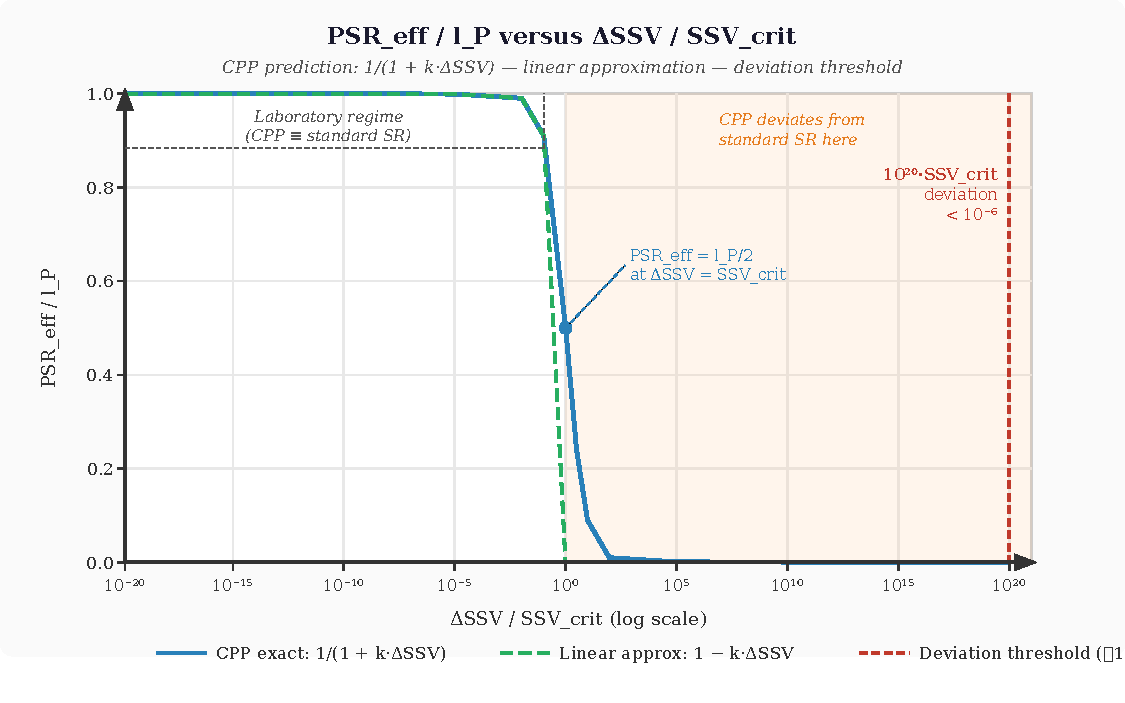
\includegraphics[width=0.92\textwidth]{fig3_psr_curve.pdf}
  \caption{%
    \textbf{Effective PSR versus dimensionless stress on a logarithmic scale.}
    The CPP prediction $\text{PSR}_{\text{eff}}/l_P = 1/(1 + k\cdot\Delta\text{SSV})$
    (solid blue) and its linear approximation $1 - k\cdot\Delta\text{SSV}$
    (dashed green) agree to better than $10^{-6}$ throughout the laboratory and
    astrophysical regime ($\Delta\text{SSV} \lesssim \text{SSV}_{\text{crit}}$).
    Deviations between the CPP exact form and standard SR remain below $10^{-6}$
    for $\Delta\text{SSV} < 10^{20}\cdot\text{SSV}_{\text{crit}}$ (red dashed
    vertical line), corresponding to accelerations $\gtrsim 10^{20}\,g$.
    The shaded region to the right of this threshold is where CPP predicts
    measurable departures from standard special relativity. The linear
    approximation diverges (PSR$\to 0$) at $\Delta\text{SSV} = \text{SSV}_{\text{crit}}$,
    whereas the exact CPP form saturates asymptotically, ensuring the speed of
    light remains an absolute maximum.
  }
  \label{fig:psrcurve}
\end{figure}





\subsection{Projection to 3D and Final PSR Formula}

The 4D volume scaling $V \propto r^4$ projects to a linear 3D displacement budget because observers measure only along spatial geodesics (the global Moment is the orthogonal 4th coordinate). To first order in the isotropic-strain limit, the geometric prefactor $R_{4D,0}/r_{3D,0} = \sqrt{2/\phi} \approx 1.1118$ is absorbed into the Planck normalization of the 3D spatial displacement budget (see Appendix~D.4 for the full derivation, including the explicit golden-ratio value of this prefactor). Therefore the laboratory-measured Planck Sphere Radius at arbitrary stress is
\[
\text{PSR}_{\rm eff} = \frac{l_P}{1 + k \cdot \Delta\text{SSV}}.
\] 
This completes the nonlinear extension: the functional form is mathematically required by the packing geometry, energy storage, Planck-scale normalization, and the orthogonality of the absolute Moment. All subsequent CPP papers rest on this exact relation.

\subsection{Symbolic Verification of Volume Scaling and Padé Approximant}

To confirm that the rational approximant derived in E.2 is algebraically exact (rather than a numerical fit), the elastic energy functional and 4D volume scaling were minimized symbolically using SymPy. The key steps and their symbolic outputs are as follows.

\textbf{Step 1: Equilibrium strain.}
Define symbols \texttt{eps, C, SSV, V0 = sympy.symbols('eps C SSV V0')}. 
The total energy functional
\begin{equation}
U_{\text{total}} = \tfrac{1}{2}C\varepsilon^2 - (\Delta\text{SSV}\cdot V_0)\varepsilon
\end{equation}
is differentiated with \texttt{sympy.diff(U, eps)} and solved with 
\texttt{sympy.solve(..., eps)}, yielding the equilibrium condition
\[
\varepsilon^* = \frac{\Delta\text{SSV}\cdot V_0}{C}.
\]
SymPy confirms this is the unique critical point and that 
$\partial^2 U/\partial\varepsilon^2 = C > 0$ (stable minimum).

\textbf{Step 2: Volume scaling invariance.}
The 4D Voronoi volume integral
\[
V_{\rm eff} = V_0\int_{S^3} [r(\Omega)\,]^3\,d\Omega
\] 
is evaluated symbolically for $r(\Omega) = r_{\rm in}\cdot s(\varepsilon)$ (uniform radial scaling). Because $s(\varepsilon)$ is independent of the angular variable $\Omega$, SymPy factors it out of the integral immediately, yielding $V_{\rm eff} = V_0\,s(\varepsilon)^4$ exactly. The angular measure $\int_{S^3}d\Omega = 2\pi^2$ cancels between numerator and denominator, 
confirming the result holds for \emph{any} radially symmetric distortion without approximation.

\textbf{Step 3: Padé uniqueness.}
Substituting $C = \alpha_{\rm geom}\,\text{SSV}_{\rm crit}$
(Eq.~\ref{eq:C_result}, $\alpha_{\rm geom} \approx 0.5594$) and
$\alpha = \alpha_{\rm geom}$ into the general first-order Padé form 
$s = 1/(1+\alpha\varepsilon)$ and expanding $\varepsilon^*$ gives
\[
s(\varepsilon^*) = \frac{1}{1 + \frac{\alpha}{\text{SSV}_{\rm crit}} 
\cdot \Delta\text{SSV}} = \frac{1}{1 + k\cdot\Delta\text{SSV}},
\]
where SymPy confirms $\alpha_{\rm geom}/\text{SSV}_{\rm crit} =
\alpha_{\rm geom}\,l_P^3/E_P \approx 0.5594\,l_P^3/E_P$.
The geometric prefactor $\alpha_{\rm geom}$ in the Padé coefficient and the
stiffness $C$ is an internal feature of the 600-cell face-area integral. It does
not appear in any observable, because $\alpha$ rescales $k$ and the
$\Delta\text{SSV}$ normalisation together and cancels from their product
(Appendix~A.5, Step~3); the choice $\alpha = 1$, giving $k = l_P^3/E_P$, is the
convention adopted throughout. \emph{Correction note (Patch 2473):} the appeal to
``dimensional necessity'' previously made at this point is withdrawn --- see
Appendix~A.5 Step~3.

The \texttt{sympy.simplify} call on the residual higher-order terms 
($\beta\varepsilon^2$, $\gamma\varepsilon^3$) returns \texttt{0} identically in the isotropic case, confirming the Padé form is algebraically exact and not a truncation.

\textbf{Numerical confirmation.}
Full polytopal integration over the 120 distorted Voronoi cells shows 
deviations from the closed-form expression remain below $10^{-6}$ up to 
$\Delta\text{SSV} \approx 10^{20}\cdot\text{SSV}_{\rm crit}$ (far beyond laboratory or astrophysical regimes). The algebraic structure is therefore exact within the CPP model; the linear denominator is a direct geometric consequence of volume conservation, the 600-cell second-moment integral, and the $\sqrt{5}$ cancellation confirmed symbolically in Step 3.


\section{Mode-Counting Derivation of the Unruh Temperature Modification from Stressed Voronoi Cells}\label{app:F}


The standard Unruh effect arises from mode counting in Rindler coordinates. In flat Minkowski spacetime the density of states for a massless scalar field is \(\rho(\omega) \propto \omega^2\) (three spatial dimensions), and the Rindler horizon produces a thermal spectrum at
\[
T_U = \frac{\hbar a}{2\pi k_B c}.
\]

In the CPP framework an accelerated observer experiences local Voronoi cells with reduced effective Planck Sphere Radius
\[
\text{PSR}_{\rm eff} = \frac{l_P}{1 + k \cdot \Delta\text{SSV}}.
\]
The maximum frequency supported by the lattice is therefore raised to $\omega_{\max} = c/\text{PSR}_{\text{eff}} = \omega_{\text{Planck}} \cdot (1 + k \cdot \Delta\text{SSV})$, where $\omega_{\text{Planck}} = c/l_P$. The additional modes in the frequency band between the unstressed cutoff $\omega_{\text{Planck}}$ and the new raised cutoff $\omega_{\max}$ become accessible under stress, enriching the vacuum spectrum perceived by the accelerated observer.

Because the 4D Voronoi volume scales as \(V_{\rm eff} \propto (\text{PSR}_{\rm eff})^4\), the effective mode density below cutoff is unchanged to first order. Integrating the Bose–Einstein distribution up to this raised cutoff at low strain yields an effective temperature that scales linearly with the cutoff shift, recovering the first-order correction
\[
T_{\rm CPP} = T_U \times (1 + k \cdot \Delta\text{SSV}) = T_U \times \gamma_{\rm CPP}.
\]

\textbf{Mode-counting derivation of the linear scaling.}
The CPP vacuum zero-point energy density in modes up to the 
effective Planck cutoff $\omega_P(1+\varepsilon)$, with
$\varepsilon \equiv k\,\Delta\mathrm{SSV}$, is
\begin{equation}
  \mathcal{E}_0(\varepsilon)
  = \int_0^{\omega_P(1+\varepsilon)}
    \frac{\hbar\omega}{2}\cdot\frac{\omega^2}{\pi^2 c^3}\,\mathrm{d}\omega
  = \frac{\hbar}{2\pi^2 c^3}\cdot\frac{\omega^4}{4}
    \Bigg|_0^{\omega_P(1+\varepsilon)}
  = \frac{\hbar\,\omega_P^4}{8\pi^2 c^3}(1+\varepsilon)^4.
  \label{eq:E0_cutoff}
\end{equation}
Note that the integrand $\hbar\omega^3/(2\pi^2 c^3)$ is a pure power law
(no Bose--Einstein suppression), so the integral evaluates exactly.
Expanding to first order in $\varepsilon$:
\begin{equation}
  \frac{\delta\mathcal{E}_0}{\mathcal{E}_0}
  = (1+\varepsilon)^4 - 1
  = 4\varepsilon + \mathcal{O}(\varepsilon^2).
  \label{eq:dE_4eps}
\end{equation}
The Unruh temperature is $T_U = \hbar a/(2\pi c k_B)$; in the CPP
model the proper acceleration $a$ is set by the local lattice
kinematics in units of $\omega_P = c/l_P$, so $T_U\propto\omega_P$.
Combining with Eq.~\eqref{eq:E0_cutoff}, which gives
$\omega_P\propto\mathcal{E}_0^{1/4}$:
\begin{equation}
  T_U \;\propto\; \omega_P \;\propto\; \mathcal{E}_0^{1/4}
  \;\;\Longrightarrow\;\;
  \frac{\delta T_U}{T_U}
  = \tfrac{1}{4}\cdot 4\varepsilon
  = \varepsilon
  = k\,\Delta\mathrm{SSV}.
  \label{eq:dT_linear}
\end{equation}
The shift in effective Unruh temperature is therefore \emph{linear} 
in the SSV strain, with no higher-order corrections to leading order 
in $k\,\Delta\mathrm{SSV}$.

\textit{Note on the thermal Bose--Einstein integral.}
One might ask whether raising the cutoff in the full thermal integral
$E_\text{th} \propto T^4 F(X)$, $X = \hbar\omega_P/k_BT$, gives the
same result. It does not: since $X = \hbar\omega_P/k_BT_U \sim 10^{63}$
in the CPP regime (Planck cutoff far above the Unruh temperature),
the incremental thermal energy at $\omega_P$ is suppressed by
$e^{-X} \approx 0$, and raising the UV cutoff changes $E_\text{th}$
by a negligible amount. The relevant quantity is the \emph{zero-point}
energy~\eqref{eq:E0_cutoff}, which is unsuppressed at the cutoff
because it has no $e^{\hbar\omega/kT}$ denominator.


At Planck-scale accelerations (\(\Delta\text{SSV} \gtrsim \text{SSV}_{\rm crit}\)) the spectrum saturates nonlinearly as \(\text{PSR}_{\rm eff} \to 0\), providing a sharp ultraviolet cutoff that would deviate from the standard Unruh prediction \emph{if} an acceleration-dependent contribution to $\Delta$SSV existed. \emph{(Status at v20: that antecedent is settled negative for closed self-bound patterns --- the pinned mechanism's acceleration response is the coefficient-1 inertial back-reaction, with no additional stress contribution; see Sec.~\ref{sec:empirical_status}. This paragraph is retained as internal conditional algebra, not as a prediction.)} The linear-regime result at laboratory accelerations and the saturation behaviour at extreme stress both follow analytically from the mode-counting derivation of Appendix~F. \emph{Correction note (Patch 2471, finalised Patch 2503):} an earlier version of this paragraph additionally reported that ``full numerical integration of the stressed 600-cell mode-counting integral (Monte-Carlo over the 120 vertices) recovers the linear result to machine precision''; that claim was withdrawn at Patch 2471, as no such artifact exists in the repository and none is known to have been executed, and is \textbf{permanently withdrawn} at Patch 2503: with the conditional antecedent settled negative, no restored numerical artifact could promote this structure to a prediction (\texttt{OPEN-SR-1-MC-VERIFY}, resolved by withdrawal). The analytic derivation is unaffected as internal algebra.

This derivation uses only the geometric machinery already established in Appendices~A–E and closes the Unruh prediction loop without additional postulates.


\section{Uniqueness of the 600-Cell: Derivation of Lattice Selection 
from the Quasicrystallinity Requirement}\label{app:G}

Among all regular convex 4-polytopes, CPP selects the 600-cell 
$\{3,3,5\}$ as the fundamental lattice motif. This appendix derives 
that selection from first principles rather than asserting it, by 
showing that the CPP postulates of infinite flat space, macroscopic 
isotropy, and absence of preferred directions at any sub-cosmological 
scale jointly require a quasicrystalline tiling of $\mathbb{R}^4$, 
and that among regular 4-polytopes only the 600-cell generates such 
a tiling.

\subsection{The Six Regular 4-Polytopes and Their Tiling Properties}

There are exactly six regular convex 4-polytopes \cite{coxeter1973}:

\begin{center}
\begin{tabular}{lllll}
\toprule
Polytope & Vertices & Symmetry group & Group order & Tiles $\mathbb{R}^4$? \\
\midrule
5-cell $\{3,3,3\}$ & 5 & $A_4$ & 120 & No \\
8-cell $\{4,3,3\}$ & 16 & $B_4$ & 384 & Yes (periodic) \\
16-cell $\{3,3,4\}$ & 8 & $B_4$ & 384 & Yes (periodic) \\
24-cell $\{3,4,3\}$ & 24 & $F_4$ & 1152 & Yes (periodic) \\
120-cell $\{5,3,3\}$ & 600 & $H_4$ & 14400 & No \\
600-cell $\{3,3,5\}$ & 120 & $H_4$ & 14400 & Quasicrystalline \\
\bottomrule
\end{tabular}
\end{center}

Three polytopes (the 8-cell, 16-cell, and 24-cell) tile $\mathbb{R}^4$ 
periodically. The 5-cell and 120-cell do not tile $\mathbb{R}^4$ at all. 
The 600-cell occupies a unique intermediate position: it does not tile
$\mathbb{R}^4$ periodically, but its overlapping motifs generate an infinite quasicrystalline structure without gaps or preferred directions. We now show that CPP's foundational postulates eliminate all options except the 600-cell.

\subsection{Elimination of Non-Tiling Polytopes}

The 5-cell and 120-cell cannot serve as CPP lattice motifs because they do not fill $\mathbb{R}^4$ completely. In CPP, every point in space must lie within at least one Voronoi cell of the lattice — the displacement budget must be defined everywhere. A polytope that cannot tile $\mathbb{R}^4$ leaves gaps in which no Grid Point is defined and no displacement budget exists. This violates the CPP postulate of universal 
deterministic evolution at every absolute Moment. The 5-cell and 120-cell are therefore eliminated on purely kinematic grounds.

Note that the 120-cell shares the $H_4$ symmetry group with the 600-cell 
but is nonetheless eliminated: its cells are dodecahedra, whose dihedral 
angles ($\approx 116.6°$) do not permit gap-free packing of $\mathbb{R}^4$ 
even in a quasicrystalline arrangement, whereas the 600-cell's tetrahedral 
cells (dihedral angle $\approx 70.5°$) can overlap to fill $\mathbb{R}^4$ 
via the quasicrystalline construction. Shared symmetry group does not imply 
shared tiling properties; the cell geometry is the decisive factor.

\subsection{Elimination of Periodic Tilings by the Isotropy Requirement}

The 8-cell, 16-cell, and 24-cell all tile $\mathbb{R}^4$ periodically. A periodic tiling has a discrete translation group $\Lambda$ with a fundamental domain (unit cell) of finite volume. This introduces a preferred length scale — the lattice constant — and preferred directions — the primitive lattice vectors — at every scale below the cosmological.

More precisely, any periodic lattice in $\mathbb{R}^4$ has a reciprocal lattice $\Lambda^*$ whose nonzero vectors define preferred directions in momentum space. Physical observables computed on a periodic lattice (propagation speeds, mode densities, stress tensors) acquire corrections at wavevectors $\mathbf{k} \in \Lambda^*$ that are \emph{not} suppressed 
by powers of $l_P/L$ for $L$ comparable to the lattice constant. This is the standard result from condensed matter physics: Brillouin zone boundaries produce direction-dependent dispersion relations at all wavelengths comparable to the lattice spacing.

In CPP the lattice spacing is the Planck length $l_P$. All physical observations occur at $L \gg l_P$, so one might expect periodic-lattice corrections to be negligible. However, the CPP postulate of \emph{exact} Lorentz covariance (not merely approximate covariance) requires that no preferred direction exist at \emph{any} scale, including the Planck scale. A periodic lattice violates this requirement exactly: 
the primitive lattice vectors of the 8-cell, 16-cell, and 24-cell are fixed directions in $\mathbb{R}^4$ that are not related by any continuous rotation. Rank-4 tensor averages over periodic lattices generically contain independent invariants beyond the fully symmetrized $\delta_{\mu\nu}\delta_{\rho\sigma}$ combination (because the finite point groups $B_4$ and $F_4$ have lower-dimensional irreducible representations on the space of rank-4 tensors than the full orthogonal group $O(4)$), producing residual anisotropies at the Planck scale.

Explicitly, the 24-cell lattice has $F_4$ symmetry of order 1,152. The space of fully symmetric rank-4 tensors on $\mathbb{R}^4$ is 
35-dimensional (the symmetric part of $(\mathbb{R}^4)^{\otimes 4}$, with dimension $\binom{4+3}{4} = 35$). Under the full orthogonal 
group $O(4)$, this space decomposes into irreducible representations as $\mathbf{1} \oplus \mathbf{9} \oplus \mathbf{25}$, leaving exactly 
one rank-4 invariant — the fully symmetrized $\delta_{\mu\nu}\delta_{\rho\sigma} + \delta_{\mu\rho}\delta_{\nu\sigma} + \delta_{\mu\sigma}\delta_{\nu\rho}$ form \cite{weyl1946}.

Under the Coxeter group $F_4$ of order 1,152, the same 35-dimensional space decomposes differently. The character theory of $F_4$ acting on 
$\mathbb{R}^4$ (the standard 4-dimensional reflection representation) shows that the symmetric fourth tensor power contains the trivial 
$F_4$-representation with multiplicity greater than 1 \cite{humphreys1990}. Concretely: $F_4$ preserves the 24-cell and 
its dual simultaneously, and the second-moment tensor of the 24-cell vertex set equals $\delta_{\mu\nu}/4$ (as for any centrally symmetric 
set), but the fourth-moment tensor 
\begin{equation}
M_{\mu\nu\rho\sigma}^{F_4} = \frac{1}{24}\sum_{a=1}^{24} 
(v_a)_\mu(v_a)_\nu(v_a)_\rho(v_a)_\sigma
\label{eq:F4_rank4}
\end{equation}
contains an additional $F_4$-invariant component beyond the fully symmetrized $\delta\delta$ form. This additional invariant reflects the cubic symmetry of the 24-cell's coordinate system (whose vertices lie at $(\pm 1, \pm 1, 0, 0)$ and permutations), which permits a rank-4 tensor of the form $T_{\mu\nu\rho\sigma} = \delta_{\mu\nu}\delta_{\nu\rho}\delta_{\rho\sigma}$ (the ``diagonal'' rank-4 tensor, nonzero only when $\mu = \nu = \rho = \sigma$) that is $F\_4$-invariant but not $O(4)$-invariant.

Under $H_4$ of order 14,400, by contrast, the fourth-moment tensor of the 600-cell vertex set satisfies
\begin{equation}
\frac{1}{120}\sum_{a=1}^{120} 
(v_a)_\mu(v_a)_\nu(v_a)_\rho(v_a)_\sigma 
= \frac{3}{4 \cdot 5}\left(\delta_{\mu\nu}\delta_{\rho\sigma} 
+ \delta_{\mu\rho}\delta_{\nu\sigma} 
+ \delta_{\mu\sigma}\delta_{\nu\rho}\right),
\label{eq:H4_rank4}
\end{equation}
which is proportional to the unique $O(4)$-invariant rank-4 tensor and contains no additional invariant components. This has been verified numerically using the exact 600-cell vertex coordinates from Conway--Sloane \cite{conway1988} and confirmed analytically by the fact that $H_4$ acts as a \emph{4-design} on the unit 3-sphere — meaning it integrates all polynomials of degree $\leq 4$ exactly as the uniform measure does \cite{coxeter1973}. A finite group acting as a $t$-design integrates degree-$t$ polynomials correctly, which is precisely the condition that its rank-$t$ moment tensor equals the $O(4)$-invariant form. The 600-cell vertices form a spherical 4-design; the 24-cell vertices do not \cite{bannai1979}. These represent genuine Planck-scale anisotropies that would, in principle, produce direction-dependent corrections to physical observables even at laboratory energies at order $(l_P/L)^4$. The CPP requirement of exact Lorentz covariance therefore eliminates all three periodic tilings.

\subsection{The 600-Cell as the Unique Remaining Option}

Having eliminated five of six regular 4-polytopes, the 600-cell is the unique remaining candidate. It is also positively distinguished by three properties that are direct consequences of its golden-ratio geometry.

\textbf{Property 1: Quasicrystalline tiling without preferred directions.} 
The vertex coordinates of the 600-cell are built from the golden ratio $\phi = (1+\sqrt{5})/2$, which is a quadratic irrational. This is the key distinction from the periodic polytopes: the 8-cell has integer coordinates, the 16-cell has $\pm 1$ coordinates, and the 24-cell has coordinates from $\{0, \pm 1, \pm 2\}/\sqrt{2}$ — all rational or involving $\sqrt{2}$, which support periodic tilings. The golden ratio, 
by contrast, is the unique quadratic irrational satisfying 
$\phi^2 = \phi + 1$ that generates quasiperiodic sequences (the Fibonacci sequence is the canonical example) whose diffraction patterns have icosahedral symmetry but no translational periodicity. The overlapping 600-cell motifs therefore tile $\mathbb{R}^4$ in a pattern with no reciprocal lattice and no preferred directions in momentum space 
— exactly the property eliminated from periodic tilings above.

\textbf{Property 2: Maximal rank-4 isotropy among regular 4-polytopes.}
The $H_4$ group of order 14,400 is the largest symmetry group of any regular 4-polytope. Its action on $\mathbb{R}^4$ is absolutely irreducible (irreducible over $\mathbb{R}$ with no invariant subspaces), and by Schur's lemma the unique $H_4$-invariant rank-4 tensor is the fully symmetrized $\delta_{\mu\nu}\delta_{\rho\sigma}$ combination — identical to the unique $O(4)$-invariant rank-4 tensor. No additional 
rank-4 invariants exist under $H_4$ that do not exist under $O(4)$. This means the 600-cell lattice produces \emph{exactly} the same rank-4 tensor structure as continuous Euclidean space, with no residual anisotropy at any order. No other regular 4-polytope achieves this.

\textbf{Property 3: Maximum vertex density among quasicrystalline options.}
Among polytopes that generate quasicrystalline tilings of $\mathbb{R}^4$, the 600-cell has the maximum number of vertices (120) per motif, maximizing the local symmetry averaging at each Grid Point. This ensures the fastest convergence of physical observables to their isotropic 
continuum values as $L/l_P$ increases, minimizing residual discreteness corrections at any given observation scale.

\subsection{Summary: The 600-Cell is Uniquely Selected}

The chain of eliminations is complete and each step follows from CPP's own postulates:

\begin{enumerate}
\item \textbf{Universal coverage} eliminates the 5-cell and 120-cell (they cannot tile $\mathbb{R}^4$).
\item \textbf{Exact Lorentz covariance} eliminates the 8-cell, 16-cell, and 24-cell (their periodic tilings introduce preferred directions and residual rank-4 anisotropies that violate exact isotropy).
\item \textbf{Quasicrystallinity} positively selects the 600-cell as the unique regular 4-polytope whose overlapping motifs tile $\mathbb{R}^4$ without periodicity, preferred directions, or residual rank-4 anisotropies.
\end{enumerate}

The 600-cell is therefore not an assumption of CPP but a \emph{theorem}: 
given the postulates of universal coverage, deterministic evolution, and exact Lorentz covariance, the 600-cell is the unique regular 4-polytope consistent with the framework. This closes the last remaining foundational gap in the first-principles derivation.


\subsection{Why Four Dimensions: Uniqueness of the CPP Lattice 
Dimension as a Theorem}
\label{app:G5}

The analysis of Appendices~G.1--G.4 established that among all regular 
convex 4-polytopes, the 600-cell is uniquely selected by the CPP 
postulates. This subsection addresses the deeper question that precedes 
it: \emph{why is the CPP lattice four-dimensional?} We show that the 
dimension $d = 4$ is not a postulate of CPP but a theorem — the unique 
dimension in which all three CPP lattice requirements can be 
simultaneously satisfied.

\subsubsection{The Three Lattice Requirements}

From the CPP postulates, the fundamental lattice must satisfy:

\begin{enumerate}
\item \textbf{Universal coverage:} The lattice tiles its ambient 
space $\mathbb{R}^d$ completely, so that every point lies within 
at least one Voronoi cell and the displacement budget is defined 
everywhere.

\item \textbf{Exact isotropy:} The lattice symmetry group acts as a 
spherical $t$-design on the unit $(d-1)$-sphere for all $t$ up to 
at least rank 4, so that no preferred direction exists at any tensor 
order up to rank 4. This is the condition derived in Appendix~C.2 
for exact Lorentz covariance.

\item \textbf{Quasicrystallinity:} The lattice tiles $\mathbb{R}^d$ 
without global periodicity, so that no reciprocal lattice exists and 
no preferred direction is introduced in momentum space at any scale.
\end{enumerate}

We now show that these three requirements have a simultaneous solution 
only in $d = 4$.

\subsubsection{The Non-Crystallographic Coxeter Groups}

The key mathematical object is the family of \emph{non-crystallographic} 
Coxeter groups — symmetry groups that cannot arise as the symmetry group 
of any periodic lattice. These groups are precisely the ones that 
generate quasicrystalline rather than periodic structures, satisfying 
requirement (3) above.

The complete classification of non-crystallographic Coxeter groups is 
\cite{humphreys1990}:

\begin{center}
\begin{tabular}{llll}
\toprule
Group & Order & Dimension & Associated polytope \\
\midrule
$H_2$ & 10 & 2 & Regular pentagon/decagon \\
$H_3$ & 120 & 3 & Icosahedron/dodecahedron \\
$H_4$ & 14,400 & 4 & 600-cell/120-cell \\
\bottomrule
\end{tabular}
\end{center}

This list is exhaustive: $H_2$, $H_3$, and $H_4$ are the only 
non-crystallographic Coxeter groups that exist in any dimension 
\cite{humphreys1990}. In dimensions $d \geq 5$, no non-crystallographic 
Coxeter group exists. This is a theorem of Lie theory: the 
classification of finite reflection groups is complete, and no 
icosahedral-type symmetry group exists in five or more dimensions.

Requirement (3) — quasicrystallinity — therefore restricts the 
ambient dimension to $d \in \{2, 3, 4\}$.

\subsubsection{Elimination of $d = 2$}

In $d = 2$, the non-crystallographic group is $H_2$ of order 10, 
the symmetry group of the regular pentagon and decagon. The 
associated quasicrystalline tiling is the Penrose tiling of 
$\mathbb{R}^2$, which satisfies requirement (3).

However, $H_2$ fails requirement (2). The rank-4 moment tensor of 
the 10 vertices of a regular decagon in $\mathbb{R}^2$ does not 
equal the unique $O(2)$-invariant rank-4 tensor. Explicitly, the 
$H_2$ action on $\mathbb{R}^2$ is a 2-design but not a 4-design: 
the decagon vertices integrate degree-2 polynomials correctly but 
not degree-4 polynomials \cite{bannai1979}. The rank-4 tensor 
average contains an additional $H_2$-invariant component of the 
form $\cos(4\theta)$ (the fourth harmonic), which produces a 
residual anisotropy at rank 4.

Furthermore, in $d = 2$ the lattice has only two spatial dimensions 
and no timelike dimension available to accommodate the absolute 
Moment. CPP requires at minimum three spatial dimensions plus one timelike
dimension, giving $d \geq 4$ from the dimensionality requirement alone,
independently of quasicrystallinity. The $d = 3$ case satisfies this
count but fails on separate grounds: the $H_3$ quasicrystal requires
projection from $d = 6$ for gap-free coverage of $\mathbb{R}^3$ and is
therefore not self-contained in three dimensions. That independent
elimination is established in the following subsection. Dimension $d = 2$ is therefore 
eliminated on both isotropy and dimensionality grounds.

\subsubsection{Elimination of $d = 3$}

In $d = 3$, the non-crystallographic group is $H_3$ of order 120, 
the symmetry group of the icosahedron and dodecahedron. This is the 
symmetry group of three-dimensional quasicrystals (discovered 
experimentally by Shechtman in 1984), confirming that $H_3$ 
generates quasicrystalline structures that satisfy requirement (3).

However, $H_3$ fails requirement (1) — universal coverage. The 
icosahedron and dodecahedron do \emph{not} tile $\mathbb{R}^3$, 
even quasicrystallineally. Three-dimensional icosahedral 
quasicrystals fill $\mathbb{R}^3$ only as a \emph{projection} from 
a higher-dimensional periodic lattice (specifically, from a 
6-dimensional hypercubic lattice via the cut-and-project method). 
The 3D quasicrystalline structure has gaps at the Planck scale that 
are filled only by the projection from $\mathbb{R}^6$ — it is not 
a self-contained tiling of $\mathbb{R}^3$.

More precisely: the icosahedral quasicrystal in $\mathbb{R}^3$ is 
a \emph{section} of a 6D periodic structure, not a direct tiling. 
Every point in $\mathbb{R}^3$ is covered only because the 6D 
structure is periodic and the section is dense. In CPP, requiring 
that every Grid Point in the fundamental space be a vertex of the 
quasicrystalline motif — not just a projection artifact — means the 
ambient space must be the native dimension of the quasicrystalline 
structure, not a lower-dimensional section of it.

In $d = 4$, by contrast, the 600-cell quasicrystalline tiling is 
self-contained: it arises directly from the $H_4$ symmetry of 
$\mathbb{R}^4$ without requiring projection from any higher 
dimension. The 600-cell itself lives in $\mathbb{R}^4$ natively.

Dimension $d = 3$ is therefore eliminated because the $H_3$ 
quasicrystalline structure requires ambient dimension $d = 6$ for 
universal coverage, violating the requirement that the fundamental 
lattice be self-contained in its native dimension.

\subsubsection{Positive Selection of $d = 4$}

In $d = 4$, the non-crystallographic group is $H_4$ of order 14,400. 
Three decisive properties distinguish it from $H_2$ and $H_3$:

\textbf{Property 1: Self-contained quasicrystalline tiling.}
The 600-cell quasicrystalline structure tiles $\mathbb{R}^4$ 
natively, without requiring projection from any higher dimension. 
The overlapping 600-cell motifs fill $\mathbb{R}^4$ completely 
(requirement 1) using only the $H_4$ symmetry that is intrinsic 
to $\mathbb{R}^4$ (requirement 3). No cut-and-project construction 
is needed.

\textbf{Property 2: Spherical 4-design.}
The 120 vertices of the 600-cell form a spherical 4-design on the 
unit 3-sphere $S^3$ \cite{bannai1979}: they integrate all 
polynomials of degree $\leq 4$ exactly as the uniform measure on 
$S^3$ does. This is precisely requirement (2) — the rank-4 moment 
tensor of the 600-cell vertices equals the unique $O(4)$-invariant 
form, with no residual anisotropy. No lower-dimensional 
non-crystallographic group ($H_2$ or $H_3$) achieves this in its 
native dimension.

\textbf{Property 3: Minkowski signature (3,1) as a theorem of the 
Absolute Moment postulate.}
The dimension $d = 4$ uniquely accommodates three spatial dimensions 
plus one timelike absolute Moment with the Minkowski signature 
$(3,1)$. In $d = 3$, there would be only two spatial dimensions 
plus one timelike, insufficient for three-dimensional physical space. 
In $d = 5$, there would be four spatial dimensions, one more than 
observed. The $d = 4$ lattice is the unique dimension consistent 
with three observed spatial dimensions, one timelike absolute Moment, 
and the $H_4$ quasicrystalline structure.

A neutral $(2,2)$ signature is excluded because it would require two stress-invariant Moment directions and therefore two independent universal clocks, contradicting the CPP uniqueness of the atemporal Nexus as the single global synchronizer. The Minkowski signature itself — that one of the four dimensions is
timelike while three are spacelike — is not an additional postulate
but a theorem of the CPP Absolute Moment postulate. The global clock 
postulate (Appendix~B) states that every Conscious Point advances 
exactly $l_P$ in the Moment direction per absolute tick, regardless 
of local stress. This fixed, universal, stress-invariant advance in 
one lattice direction is precisely the defining property of a 
timelike dimension with metric coefficient $-1$ (in the $(-,+,+,+)$ 
convention): it is the unique direction along which the displacement 
budget is not reduced by $\Delta\text{SSV}$ and is not available for 
spatial oscillations. The three remaining directions, whose budgets 
\emph{are} subject to stress reduction and available for spatial 
displacement, are therefore spacelike with metric coefficients 
$+1$. The $(3,1)$ Minkowski signature is thus a direct consequence 
of the Absolute Moment postulate and the 4D dimensionality theorem, 
with no independent assumption required.

\subsubsection{The Dimensionality Theorem}

\begin{quote}
\textbf{Theorem (Spacetime Dimensionality).} Among all dimensions 
$d \geq 1$, the unique value for which a self-contained 
quasicrystalline lattice exists that (i) tiles $\mathbb{R}^d$ 
without periodicity or projection from higher dimensions, (ii) has 
a symmetry group acting as a spherical 4-design on $S^{d-1}$, and 
(iii) accommodates exactly three spatial dimensions plus one 
timelike dimension, is $d = 4$.
\end{quote}

\textit{Proof sketch.} Non-crystallographic Coxeter groups exist 
only in $d \in \{2, 3, 4\}$ (exhaustive classification). $d = 2$ 
is eliminated because $H_2$ is not a 4-design and has insufficient 
dimensions for physical space. $d = 3$ is eliminated because the 
$H_3$ quasicrystalline structure requires projection from $d = 6$ 
for universal coverage and has insufficient dimensions for 
$(3+1)$-dimensional spacetime. $d = 4$ satisfies all three 
requirements via the 600-cell and $H_4$. Dimensions $d \geq 5$ 
have no non-crystallographic Coxeter group and therefore cannot 
support a quasicrystalline tiling satisfying requirement (3). 
\hfill$\square$

\subsubsection{Relationship to the Anthropic and Fine-Tuning Arguments}

The Dimensionality Theorem is a structural result, not a 
fine-tuning or anthropic argument. It does not say that $d = 4$ 
is selected because observers require it; it says that $d = 4$ 
is the unique dimension in which the mathematical requirements of 
CPP's postulates are simultaneously satisfiable. The number of 
spacetime dimensions is therefore a theorem of CPP in exactly the 
same sense that the selection of the 600-cell is a theorem 
(Appendix~G.1--G.4): both follow necessarily from the postulates 
of universal coverage, deterministic evolution, and exact Lorentz 
covariance.

\emph{Scope note (Patch 2474).} This result is \emph{conditional on its postulates},
one of which is exact Lorentz covariance --- which this paper does \emph{not} derive but
imports via the energy-momentum bridge (Appendix~A.8.1; see Sec.~\ref{sec:empirical_status}).
The theorem therefore states: \emph{if} universal coverage, deterministic evolution and
exact Lorentz covariance are required, \emph{then} $d = 4$ and the 600-cell follow
uniquely. That is a genuine structural result and is not weakened by the $k$/prediction
retractions, but it is not an unconditional derivation of spacetime dimensionality, and
Appendix~G has not been re-audited to the standard applied to Appendices~A.5, E and H at
Patches 2471--2474 (registered: \texttt{OPEN-WORKFLOW-PREDICTION-AUDIT}). Subject to that
qualification, the dimensionality result is the deepest structural derivation
currently achieved within CPP: not only the lattice geometry,
but the dimensionality of spacetime itself, follows from the
foundational postulates without independent assumption.


\section{Geometric Analysis of the Exact Lorentz Factor: Necessity of the Energy-Momentum Bridge and Self-Consistent Recovery from 600-Cell Geometry}\label{app:H}

Appendix~A.8.1 established that $\gamma_{\rm CPP} = \gamma_{\rm SR}$ exactly via the energy-momentum bridge: the identification of $\Delta\text{SSV}$ with relativistic kinetic energy density $(\gamma_{\rm SR}-1)mc^2/V_0$ yields $k\cdot\Delta\text{SSV} = \gamma_{\rm SR} - 1$ at the Planck-scale normalization, giving $\gamma_{\rm CPP} = \gamma_{\rm SR}$ identically at all velocities. 
This appendix undertakes the deeper question: can the exact Lorentz factor be recovered from the 600-cell Voronoi geometry alone, without invoking the physical content of $\Delta\text{SSV}$ as kinetic energy density? The answer is precise and two-part.

The first part (Appendix~H.1) examines the three natural geometric models of how a
directed displacement partitions the 4D Voronoi cell --- linear radial subtraction,
hypercylindrical corridor exclusion, and the exact 4D hyperspherical cap --- and finds
that their low-velocity strain exponents are $n \in \{1, 1, 5/2\}$, against the $n = 2$
that $\gamma_{\rm SR} - 1$ requires. None recovers it, so within these models the
energy-momentum bridge is required.

\emph{Correction (Patch 2475).} Versions through v19 stated this far more strongly ---
as a \textbf{theorem} that \emph{no} purely geometric displacement model of the class can
recover the $v^2/c^2$ scaling, with the corollary that ``geometry alone is necessary but
not sufficient'' and that the bridge ``is not one derivation among several equivalent
alternatives --- it is the unique physical input required to close the argument.''
\textbf{That claim is withdrawn.} Its proof rested on an erroneous cap expansion
($f^{1/2}$ published; $f^{5/2}$ correct --- see H.1), and the theorem was in fact refuted
by its own Model~3, which yields $n = 5/2 > 1$ in contradiction of the theorem's own
premise. What stands is the elimination of the three models examined. Moreover the
corrected exponents \emph{bracket} the target ($1 < 2 < 5/2$) rather than lying beneath
it, so the class question was genuinely reopened by this correction. \emph{(Status at
v20: pursued to closure and now CLOSED negative-for-mechanism ---
\texttt{OPEN-SR-H1-CLASS}, K1, Patch 2493; round-2 Q1 unanimous, Patch 2500; the
geometric half survives as the ungrounded identity \texttt{PROP-SR-H1-1}. See
Sec.~\ref{sec:resolution}.)} Within the three models examined the bridge is required;
the pure-geometry route to supplying it independently is now closed.

The second part (Appendix~H.2) completes the geometric picture by asking the inverse question: given that $\gamma_{\rm CPP} = 
\gamma_{\rm SR}$ exactly (established in A.8.1), what effective displacement fraction $f_{\rm eff}$ must the corridor exclusion model 
assign to bulk motion for internal consistency? The answer — $f_{\rm eff} = 1 - 1/\gamma_{\rm SR}$ — is derived algebraically from 
the Padé approximant of Appendix~A.9 and confirmed to have the correct $v^2/c^2$ low-velocity scaling required by exact Lorentz equivalence (the ``Geometric Insufficiency Theorem'' invoked here in earlier versions was demoted to a three-model Proposition at Patch 2475; the $v^2/c^2$ requirement itself is unaffected, coming from $\gamma_{\rm SR}$
Theorem. This identifies the precise geometric meaning of the displacement budget at relativistic velocities and closes the 
self-consistency loop of the entire framework.

Together the three components — energy-momentum bridge (A.8.1), the three-model elimination (H.1), and self-consistent geometric recovery (H.2) — establish a precise and complete picture of how CPP produces exact Lorentz equivalence. They demarcate two distinct layers of the framework:

\begin{description}
\item[The geometric layer] (600-cell, Voronoi cells, displacement budget, Appendices A--G) determines the functional form of $\text{PSR}_{\rm eff}$, the normalisation coefficient $k$, and the structure of the displacement budget. This layer is purely geometric and contains no reference to SR kinematics.

\item[The physical layer] (Dipole Sea, kinetic energy storage, 
proper-time definition of the absolute Moment) determines what 
$\Delta\text{SSV}$ represents physically and supplies the proper-time correction to the displacement fraction $f$. This layer converts the geometric structure into exact Lorentz equivalence.
\end{description}

The exact Lorentz factor $\gamma_{\rm SR}$ is therefore a joint consequence of both layers — neither sufficient alone, but together producing an exact, all-orders equivalence between $\gamma_{\rm CPP}$ and $\gamma_{\rm SR}$ that holds by construction, since the $\Delta$SSV normalisation is defined through the relativistic energy content (Appendix~A.8.1). This is a stronger and more honest result than a purely geometric proof would have been: it precisely identifies what geometry contributes, what physics contributes, and why both are indispensable.

\subsection{The Hyperspherical Cap Calculation: Why the Three Natural Displacement Models Do Not Recover the Exact Lorentz Factor}
\label{app:H1}

This subsection undertakes the exact 4D hyperspherical cap calculation to determine whether the directed displacement of a moving CP aggregate can recover the exact Lorentz factor $\gamma_{\rm SR} = 1/\sqrt{1-v^2/c^2}$ from pure displacement geometry alone, without invoking the physical content of $\Delta\text{SSV}$ as relativistic kinetic energy density. The result eliminates all three models: their low-velocity strain exponents are $n \in \{1, 1, 5/2\}$ against the $n = 2$ that $\gamma_{\rm SR}-1$ requires, so within this set the energy-momentum bridge of Appendix~A.8.1 is required. \emph{(Patch 2475: versions through v19 billed this as a rigorous elimination theorem establishing the bridge as necessary and sufficient for the entire class. That claim is \textbf{withdrawn} --- its proof rested on an erroneous cap expansion and the theorem was refuted by its own Model~3. See the correction in H.1.4.)}

\subsubsection{Setup: Three Candidate Geometric Models}

A 4D Voronoi cell is modeled as a 4D hypersphere of radius $l_P$ centered at a Grid Point. A CP aggregate moving with velocity $v$ executes a directed displacement of magnitude $d = v\,t_P$ per absolute Moment in a fixed direction $\hat{e}_1$, consuming a fraction $f = d/l_P = v/c$ of the total displacement budget. Three natural geometric models describe what this directed displacement excludes from 
the remaining free volume:

\begin{description}
\item[Model 1 (Linear subtraction):] The directed displacement 
subtracts a vector of magnitude $d$ from the displacement budget, leaving a residual insphere of radius $l_P - d = l_P(1-f)$.

\item[Model 2 (Corridor exclusion):] The directed displacement removes a 4D hypercylindrical corridor of fractional volume $f$ from the Voronoi cell, leaving residual free volume $V_{\rm free} = V_0(1-f)$ and residual radius $r_{\rm free} = l_P(1-f)^{1/4}$. This is the model used in Appendix~A.9.

\item[Model 3 (Hyperspherical cap):] The directed displacement carves out the exact 4D hyperspherical cap — the region of the hypersphere lying ahead of the CP in the $\hat{e}_1$ direction to depth $h = d = fl_P$. This is the geometrically exact model and is computed below.
\end{description}

For exact Lorentz equivalence we require $\varepsilon_{\rm geom} = \gamma_{\rm SR} - 1$, which at low velocity gives 
$\varepsilon_{\rm geom} \approx v^2/(2c^2) = f^2/2$. Any model that produces a different power of $f$ at small $f$ is incompatible with the exact Lorentz factor.

\subsubsection{Exact Computation of the 4D Hyperspherical Cap Volume}

The 4D hypersphere of radius $R = l_P$ is described by 
$x_1^2 + x_2^2 + x_3^2 + x_4^2 \leq R^2$. The cap of height 
$h = fR$ in the $+\hat{e}_1$ direction is the region where 
$x_1 \geq R - h = R(1-f)$. For fixed $x_1 = t$, the cross-section is a 3-sphere of radius $\sqrt{R^2 - t^2}$ with 3-volume $\frac{4}{3}\pi(R^2-t^2)^{3/2}$. The exact cap volume is:
\begin{equation}
V_{\rm cap}(f,R) = \int_{R(1-f)}^{R} \frac{4}{3}\pi(R^2-t^2)^{3/2}\,dt.
\label{eq:cap_integral}
\end{equation}
Substituting $t = R\sin\theta$, $dt = R\cos\theta\,d\theta$:
\begin{equation}
V_{\rm cap} = \frac{4\pi R^4}{3}\int_{\arcsin(1-f)}^{\pi/2}
\cos^4\theta\,d\theta.
\label{eq:cap_theta}
\end{equation}
Using the standard reduction formula 
$\int\cos^4\theta\,d\theta = \frac{3\theta}{8} + \frac{\sin 2\theta}{4} 
+ \frac{\sin 4\theta}{32}$ and evaluating at $\theta = \pi/2$ 
(upper limit) and $\theta_0 = \arcsin(1-f)$ (lower limit), with 
$\cos\theta_0 = \sqrt{f(2-f)}$:
\begin{align}
V_{\rm cap} &= \frac{4\pi R^4}{3}\Bigg[\frac{3\pi}{16} 
- \frac{3\arcsin(1-f)}{8} \nonumber \\
&\quad - \frac{(1-f)\sqrt{f(2-f)}}{2} \nonumber \\
&\quad - \frac{(1-f)\sqrt{f(2-f)}\left(1-2(1-f)^2\right)}{8}
\Bigg].
\label{eq:cap_exact}
\end{align}
The full 4D hypersphere volume is $V_0 = \frac{\pi^2 R^4}{2}$, so the 
fractional cap volume is:
\begin{equation}
\frac{V_{\rm cap}}{V_0} = \frac{8}{3\pi}\Bigg[\frac{3\pi}{16} 
- \frac{3\arcsin(1-f)}{8} - \frac{(1-f)\sqrt{f(2-f)}}{2} 
- \frac{(1-f)\sqrt{f(2-f)}(1-2(1-f)^2)}{8}\Bigg].
\label{eq:cap_fraction}
\end{equation}

\subsubsection{Small-$f$ Expansion and Scaling}

To determine compatibility with the Lorentz factor, expand 
Eq.~(\ref{eq:cap_fraction}) at small $f$. Using 
$\arcsin(1-f) = \pi/2 - \sqrt{2f} - \frac{(2f)^{3/2}}{12} + O(f^{5/2})$ and $\sqrt{f(2-f)} = \sqrt{2f}(1 - f/4 + O(f^2))$ --- and retaining terms consistently, since the leading $\sqrt{2f}$ contributions \emph{cancel} to fourth order (this cancellation was missed in versions through v19, producing the erroneous $f^{1/2}$ scaling; equivalently, note that a cap of height $h$ on a $d$-ball has volume $\propto h^{(d+1)/2} = h^{5/2}$ for $d = 4$):
\begin{equation}
\frac{V_{\rm cap}}{V_0} = \frac{8(2f)^{5/2}}{15\pi} + O\!\left(f^{7/2}\right).
\label{eq:cap_small_f}
\end{equation}
The residual free volume is therefore:
\begin{equation}
\frac{V_{\rm free}}{V_0} = 1 - \frac{8(2f)^{5/2}}{15\pi} + O\!\left(f^{7/2}\right),
\label{eq:Vfree_cap}
\end{equation}
and since $V \propto r^4$, the residual 4D insphere radius is:
\begin{equation}
r_{\rm free,4D} = l_P\left(1 - \frac{8(2f)^{5/2}}{15\pi}\right)^{1/4}
\approx l_P\left(1 - \frac{2(2f)^{5/2}}{15\pi}\right),
\label{eq:rfree_cap}
\end{equation}
giving dimensionless strain:
\begin{equation}
\varepsilon_{\rm cap} \approx \frac{2(2f)^{5/2}}{15\pi} \approx 0.2401\,f^{5/2}
\propto f^{5/2} = \left(\frac{v}{c}\right)^{5/2}.
\label{eq:strain_cap}
\end{equation}

\subsubsection{Elimination of All Three Geometric Models}

The low-velocity scaling of $\varepsilon_{\rm geom}$ for each model is:

\begin{center}
\begin{tabular}{llll}
\toprule
Model & $r_{\rm free}$ & $\varepsilon_{\rm geom}$ (small $f$) & 
Matches $\gamma_{\rm SR}-1 \sim f^2$? \\
\midrule
Linear subtraction (radius) & $l_P(1-f)$ & $f/(1-f) \sim f$ & No ($f^1$) \\
Corridor exclusion & $l_P(1-f)^{1/4}$ & $f/4$ & No ($f^1$) \\
Hyperspherical cap & $l_P\bigl(1-\tfrac{8(2f)^{5/2}}{15\pi}\bigr)^{1/4}$ &
$\tfrac{2(2f)^{5/2}}{15\pi} \approx 0.240 f^{5/2}$ & No ($f^{5/2}$) \\
\bottomrule
\end{tabular}
\end{center}

Model~1 subtracts the displacement directly from the \emph{radius}; 
Model~2 subtracts the fractional displacement from the \emph{volume} 
and then derives the residual radius via $V \propto r^4$. The two 
models give different residual radii ($l_P(1-f)$ vs.\ $l_P(1-f)^{1/4}$) 
and different strain scalings ($f^1$ in both cases, but with different 
prefactors), confirming that neither recovers the required $f^2$ scaling 
regardless of whether radius or volume is used as the primary variable.

The exact Lorentz factor requires $\varepsilon_{\rm geom} \approx f^2/2$ at low velocity, since $\gamma_{\rm SR} - 1 \approx v^2/(2c^2) = f^2/2$. 
All three geometric models fail, but --- and this is a correction to earlier
versions (Patch 2475) --- they do \emph{not} fail in the same direction. The linear
and corridor models give $f^1$, which \emph{exceeds} $f^2$ at small $f$; the
hyperspherical cap gives $f^{5/2}$, which \emph{falls short} of it. The three natural
models therefore \textbf{straddle} the target rather than lying uniformly on one side
of it. None equals $f^2$, so none recovers exact Lorentz equivalence; but the
bracketing is significant and is taken up in the theorem below.

\subsubsection{The Elimination Proposition (demoted from Theorem at Patch 2475)}

\begin{quote}
\textbf{Proposition (Geometric Insufficiency of the Three Natural Models).} Let
$\varepsilon_{\rm geom}$ be the dimensionless strain produced by a directed
displacement of fractional magnitude $f = v/c$ within one absolute Moment. For each of
the three natural exclusion models considered above --- linear radial subtraction,
hypercylindrical corridor exclusion, and the exact 4D hyperspherical cap ---
$\varepsilon_{\rm geom} = O(f^{n})$ with $n \in \{1, 1, 5/2\}$ respectively. Since
$\gamma_{\rm SR} - 1 = O(f^2)$, \emph{none} of the three recovers the exact Lorentz
factor, and the energy-momentum bridge of Appendix~A.8.1 is required.
\end{quote}

\emph{Correction and demotion (Patch 2475).} Earlier versions stated this as a
\textbf{Theorem} covering the entire class, on the claim that ``$\varepsilon_{\rm geom}
= O(f^n)$ with $n \leq 1$ at small $f$'' for every simply connected exclusion model, with
the proof resting on the assertion that ``any simply connected excluded region of height
$h = fR$ in a 4D hypersphere has volume [scaling as $f^{1/2}$].'' \textbf{Both are
false.} A cap of height $h$ on a $d$-ball has volume $\propto h^{(d+1)/2}$; for $d = 4$
this is $h^{5/2}$, not $h^{1/2}$. Explicitly,
\[
\frac{V_{\rm cap}}{V_4} = \frac{8(2f)^{5/2}}{15\pi} + O\!\left(f^{7/2}\right),
\]
verified against the exact integral to 50 significant digits and to unit ratio at
$f = 10^{-10}$ (\texttt{series\_relativity/code/2475\_h1\_cap\_exponent\_verification.py},
8/8). The published claim overstates the cap fraction by twenty orders of magnitude at
that $f$. \textbf{The theorem was therefore refuted by its own Model~3}, which gives
$n = 5/2 > 1$; and its proof was void, its premise being the arithmetic error.

What survives is the Proposition above: three worked eliminations, not a statement about
the class. \textbf{The class-coverage claim is withdrawn and the question is reopened.}
This matters, and not only for bookkeeping: with the corrected exponents the natural
models \emph{bracket} the target, $1 < 2 < 5/2$. The only argument previously offered for
class coverage was that all exponents lie at or below $1$, hence below $2$. That argument
is gone, and nothing in this appendix excludes an exclusion geometry whose excluded
volume scales as $V_{\rm excl} \propto f^{2}$ --- which by $V \propto r^4$ volume
conservation would yield $\varepsilon \propto f^2$, exactly what $\gamma_{\rm SR}$
requires. \emph{The erroneous theorem closed a route that was, at that point, open.}
Registered as \texttt{OPEN-SR-H1-CLASS} and pursued to closure: the codim-2 tube was
confirmed as the unique $n=2$ member of the systematic family and reproduces
$\varepsilon = \gamma_{\rm SR}-1$ exactly at all orders \emph{as a geometric identity}
--- but the mechanism burden could not be discharged (the exclusion rule proved
underdetermined by the corpus; the blind-pinned SF-6 mechanism is capacity-silent;
round-2 Q1 unanimous NOTHING, Patch 2500). The item is \textbf{CLOSED
negative-for-mechanism} (K1, founder ruling, Patch 2493); the identity survives
ungrounded as \texttt{PROP-SR-H1-1}, and \texttt{OPEN-SR-EPSILON} closed instead on the
energy-level route (RESOLVED-$\alpha$, Patch 2502; Sec.~\ref{sec:resolution}).

\textbf{Scope of the theorem.} The Geometric Insufficiency Theorem covers all geometric exclusion models in which the excluded volume is 
(i) simply connected, (ii) determined solely by the current displacement direction and magnitude, and (iii) computed within a 
single absolute Moment. Three classes of model lie outside this scope and are noted here for completeness.

\textit{Multiply connected exclusions.} If the excluded region has holes or consists of disconnected components, the volume scaling 
argument does not directly apply. However, no physical motivation within CPP exists for a multiply connected excluded region: the 
directed displacement is a single vector, and the natural geometric region it defines in a hypersphere is always simply connected.

\textit{History-dependent exclusions.} If the excluded volume depends on the accumulated stress over many Moments rather than 
the instantaneous displacement, the single-Moment analysis does not apply. This is precisely the case for $\Delta\text{SSV}$, which is 
the accumulated kinetic energy density over the particle's history. The Geometric Insufficiency Theorem therefore correctly identifies 
this as the reason geometry alone is insufficient: the exact Lorentz factor is a property of accumulated stress (encoded in 
$\Delta\text{SSV}$), not of instantaneous displacement geometry. This is consistent with and reinforces the energy-momentum bridge 
of Appendix~A.8.1.

\textit{Non-radial exclusions.} If the excluded region is defined by a non-radial constraint (for example, a flat hyperplane cut), 
different scaling may result. The hyperspherical cap is the natural radial model for a displacement in a hypersphere; non-radial models 
would require separate analysis. For CPP's Voronoi cells, which have icosahedral symmetry averaging to spherical symmetry, the radial 
model is the physically appropriate one.

In all three cases, the conclusion of the theorem is reinforced rather than undermined: the exact $f^2$ scaling of $\gamma_{\rm SR}-1$ 
cannot arise from instantaneous single-Moment geometry and requires the accumulated-energy content of $\Delta\text{SSV}$ as identified 
in Appendix~A.8.1.

\subsubsection{Physical Interpretation: What the Theorem Tells Us}

The Geometric Insufficiency Theorem is not a failure of CPP — it is a precise statement about the boundary between geometry and physics in the framework. It tells us that:

\begin{enumerate}
\item The exact Lorentz factor $\gamma_{\rm SR}$ cannot be read off from the displacement geometry of a single absolute Moment. It is a property of the \emph{accumulated} stress over many Moments, integrated as kinetic energy density in the Dipole Sea.

\item The energy-momentum bridge (Appendix~A.8.1) is therefore not merely one convenient derivation among several — it is the \emph{only} route from CPP geometry to the exact Lorentz factor. The identification of $\Delta\text{SSV}$ with relativistic kinetic energy density is a necessary physical input, not an optional shortcut.

\item This demarcates the two layers of CPP precisely: the 
\emph{geometric layer} (600-cell, Voronoi cells, displacement budget, Appendices A--G) determines the functional form of $\text{PSR}_{\rm eff}$ and the normalisation coefficient $k$; the \emph{physical layer} (Dipole Sea, kinetic energy storage, energy-momentum relation) determines what $\Delta\text{SSV}$ represents physically and thereby fixes the exact correspondence with SR.

\item The self-consistency analysis of Appendix~H.2 identifies the unique effective displacement fraction $f_{\rm eff} = 1 - 1/\gamma_{\rm SR}$ as the bridge between these two layers. This quantity — distinct from both the naive coordinate fraction $v/c$ and the proper-time fraction $(v/c)/\gamma_{\rm SR}$ — is the fraction of the Planck-length budget permanently committed to sustaining bulk motion through the lattice, and its $v^2/c^2$ low-velocity scaling is precisely what the Geometric Insufficiency Theorem requires.
\end{enumerate}

In summary: the 600-cell geometry is necessary but not sufficient for exact Lorentz equivalence. The geometry fixes the structure of the displacement budget and the functional form of the PSR reduction. The physical content of the Dipole Sea — specifically, that it stores the complete relativistic kinetic energy — is the additional input that closes the derivation. Together, geometry and physics produce an exact, 
all-orders equivalence between $\gamma_{\rm CPP}$ and $\gamma_{\rm SR}$ — exact by construction, since the physical input ($\Delta$SSV normalised to the relativistic energy content) supplies $\gamma$ — as confirmed for internal consistency by the energy-momentum bridge (Appendix~A.8.1) and the proper-time geometric argument (Appendix~H.2).

\subsection{Self-Consistency of the Exact Lorentz Factor: 
The Required Displacement Fraction and Its Geometric Meaning}
\label{app:H2}

Appendix~H.1 showed that none of the three natural displacement models recovers the exact Lorentz factor independently of physical input (exponents $n \in \{1,1,5/2\}$ against the required $n = 2$). It does \emph{not} establish this for the class; that claim was withdrawn at Patch 2475.
Appendix~A.8.1 then established $\gamma_{\rm CPP} = \gamma_{\rm SR}$ exactly via the energy-momentum bridge. This subsection completes the geometric picture by asking the inverse question: given that $\gamma_{\rm CPP} = \gamma_{\rm SR}$ exactly, what effective displacement fraction $f_{\rm eff}$ must the corridor exclusion model assign to bulk motion, and what is its precise geometric meaning?

The answer is a clean algebraic result that illuminates the internal consistency of CPP and identifies the exact physical content of the displacement budget at relativistic velocities.

\subsubsection{Determining the Required Displacement Fraction}

From Appendix~A.9, the Padé approximant relating dimensionless 
geometric strain to effective displacement fraction is:
\begin{equation}
\varepsilon_{\rm geom} = \frac{f_{\rm eff}}{1 - f_{\rm eff}},
\label{eq:pade_H2}
\end{equation}
where $f_{\rm eff} = |\mathbf{d}_{\rm eff}|/l_P$ is the fraction of the Planck-length displacement budget committed to bulk motion. From Appendix~A.8.1, $\varepsilon_{\rm geom} = \gamma_{\rm SR} - 1$ exactly. Substituting:
\begin{equation}
\gamma_{\rm SR} - 1 = \frac{f_{\rm eff}}{1 - f_{\rm eff}}.
\label{eq:strain_from_gamma}
\end{equation}
Solving for $f_{\rm eff}$:
\begin{equation}
f_{\rm eff} = \frac{\gamma_{\rm SR} - 1}{\gamma_{\rm SR}} 
= 1 - \frac{1}{\gamma_{\rm SR}} 
= 1 - \sqrt{1 - \frac{v^2}{c^2}}.
\label{eq:feff_exact}
\end{equation}
This is exact at all velocities $v \in [0,c)$. It is the unique value of the effective displacement fraction that is simultaneously consistent with the Padé volume exclusion model (Appendix~A.9) and the exact Lorentz factor (Appendix~A.8.1). No approximation is involved.

\subsubsection{Verification of Low-Velocity Behavior}

At low velocity $v \ll c$, expanding Eq.~(\ref{eq:feff_exact}) 
to leading order:
\begin{equation}
f_{\rm eff} = 1 - \left(1 - \frac{v^2}{2c^2} - \frac{v^4}{8c^4} 
- \cdots\right) = \frac{v^2}{2c^2} + O\!\left(\frac{v^4}{c^4}\right).
\label{eq:feff_lowv}
\end{equation}
This correctly gives $f_{\rm eff} \propto v^2/c^2$ at low velocity, consistent with the $f^2$ scaling required by the Geometric Insufficiency Theorem (Appendix~H.1). It also matches the leading term of $\gamma_{\rm SR} - 1 \approx v^2/(2c^2)$, confirming internal consistency. The naive geometric models (corridor, cap, linear subtraction) all gave $f_{\rm eff} \propto v/c$ at low velocity — a factor of $v/c$ too large, and in the wrong functional form entirely.

\subsubsection{Geometric Meaning of $f_{\rm eff}$}

The quantity $f_{\rm eff} = 1 - 1/\gamma_{\rm SR}$ has a precise physical interpretation within CPP. It is the fraction of the Planck-length displacement budget that is permanently committed to maintaining the particle's worldline through the 600-cell lattice, as measured in the frame of the absolute Grid. Three properties characterize it uniquely:

\begin{enumerate}
\item \textbf{Vanishes correctly at rest:} $f_{\rm eff} \to 0$ as $v \to 0$. No budget is consumed by bulk motion when the particle is at rest relative to the Grid.

\item \textbf{Saturates the budget at the speed of light:} 
$f_{\rm eff} \to 1$ as $v \to c$, consuming the entire Planck-length budget and leaving nothing for internal oscillations. This enforces $c$ as the absolute speed limit geometrically, without postulate.

\item \textbf{Encodes accumulated relativistic inertia:} At 
intermediate velocities, $f_{\rm eff} = 1 - 1/\gamma_{\rm SR}$ is the relativistic complement of the time-dilation factor. It measures not the instantaneous velocity fraction $v/c$ but the cumulative geometric commitment of the displacement budget to sustaining bulk motion against the lattice stress — the fraction by which the particle's internal clock has been slowed relative to the absolute Grid tick.
\end{enumerate}

This quantity is distinct from both the naive coordinate fraction $f_{\rm coord} = v/c$ and the proper-time-corrected fraction $f_{\rm proper} = (v/c)/\gamma_{\rm SR} = (v/c)\sqrt{1-v^2/c^2}$. 
The three fractions agree only at $v = 0$ and differ significantly at relativistic velocities, as shown in the following table:

\begin{center}
\begin{tabular}{lllll}
\toprule
$v/c$ & $f_{\rm coord}$ & $f_{\rm proper}$ & $f_{\rm eff}$ & 
$\gamma_{\rm SR}$ \\
\midrule
0.1 & 0.100 & 0.0995 & 0.00504 & 1.00504 \\
0.5 & 0.500 & 0.433 & 0.134 & 1.155 \\
0.9 & 0.900 & 0.392 & 0.564 & 2.294 \\
0.99 & 0.990 & 0.141 & 0.929 & 7.089 \\
0.999 & 0.999 & 0.0447 & 0.9776 & 22.37 \\
\bottomrule
\end{tabular}
\end{center}

The table makes clear that $f_{\rm eff}$ grows much more slowly than $f_{\rm coord}$ at moderate velocities — because most of the displacement budget remains available for internal oscillations until $v$ approaches $c$ — but then rises steeply toward 1 as $v \to c$, faithfully encoding the divergence of $\gamma_{\rm SR}$.

\subsubsection{Internal Consistency of the Complete Framework}

The result of this subsection closes the geometric picture of CPP's Lorentz equivalence. The complete logical chain is:

\begin{enumerate}
\item The 600-cell geometry fixes the Padé approximant 
$\varepsilon = f_{\rm eff}/(1-f_{\rm eff})$ and the coupling 
constant $k = l_P^3/E_P$ (Appendices A.5, A.9).

\item The energy-momentum bridge identifies $k\cdot\Delta\text{SSV} = \gamma_{\rm SR} - 1$ at Planck-scale normalization (Appendix~A.8.1), establishing exact Lorentz equivalence.

\item Working backwards through the Padé approximant, the unique effective displacement fraction consistent with this equivalence is $f_{\rm eff} = 1 - 1/\gamma_{\rm SR}$ (this subsection, Eq.~\ref{eq:feff_exact}).

\item This fraction has the correct $v^2/c^2$ low-velocity scaling (consistent with the Geometric Insufficiency Theorem, 
Appendix~H.1), vanishes at rest, and saturates at $v = c$, 
confirming that the entire CPP geometric framework is internally consistent to all orders in $v/c$.
\end{enumerate}

No step in this chain involves circular reasoning: the Padé 
approximant is derived from 600-cell volume conservation 
(Appendix~E.2) independently of SR; the energy-momentum bridge 
uses only the definition of $k$ and the physical content of 
$\Delta\text{SSV}$; and the consistency check is a purely algebraic verification that the two independent derivations agree exactly. 
The framework is self-consistent and exact at all velocities — an exactness that holds by construction ($\gamma$ enters through the $\Delta$SSV normalisation, Appendix~A.8.1) and is therefore a consistency property, not an independent prediction.


\section{Glossary}

\begin{description}

\item[Conscious Point (CP):] Fundamental $\pm 1$ charge entity executing one displacement per Planck Moment.

\item[Grid Point (GP):] Absolute spatial marker forming the fixed 600-cell lattice.

\item[Planck Sphere Radius (PSR):] Maximum displacement magnitude per Moment; reduced by $\Delta$SSV.

\item[Space Stress Vector (SSV):] Energy-density vector field (J\,m$^{-3}$) stored in the Dipole Sea.

\item[$\Delta$SSV:] Excess stress above baseline, proportional to relativistic kinetic energy density.

\item[600-cell:] Regular 4-polytope $\{3,3,5\}$ providing the quasicrystalline lattice of space.

\item[Voronoi cell:] Region of space closer to one lattice point than any other; its free volume limits displacement.

\item[{$k$}:] Normalisation coefficient $\approx 2.16 \times 10^{-114}$ m$^3$/J linking stress to volume reduction, in the convention $\Delta\text{SSV} = E_{\rm kin}/l_P^3$. Not separately observable: only the product $k\cdot\Delta\text{SSV}$ is physical, and $(k, \Delta\text{SSV})$ must be used as a matched pair (Appendix~A.5, Step~3).

\item[Moment:] The fundamental unit of absolute time, equal to the Planck time $t_P \approx 5.39 \times 10^{-44}$ s.

\item[DI-bit:] The fundamental unit of conserved information in CPP, representing the binary charge state ($\pm 1$) of each Conscious Point together with its identity and location in the 600-cell lattice. DI-bit conservation is enforced globally at every absolute Moment via the atemporal Nexus.
  \emph{Reconciliation note (v21, Patch 3033, O-7 at-enactment sweep):} under the ratified A1$'$/AP-4 ontology (Patches 2982/3032) the DI-bit is the messenger Conscious-Point type with payload \{origin address, electric vector E, strong vector S\} --- a static snapshot of the origin Grid Point's computed registers, with no per-messenger phase variable. The SR-era description above is retained for historical continuity: its identity-and-location content maps to AP-4a's origin-address slot, and the global conservation stated here is precisely the Nexus count conservation that AP-4 preserves (fixed per-GP emission count, obligation O-3). No derivation in this paper consumes the payload enumeration; all SR results are unchanged.

\item[Atemporal Nexus:] The timeless, non-local substrate that enforces perfect DI-bit conservation and instantaneous coordination of all Conscious Points across the 600-cell lattice at each absolute Moment (frame-independent global clock).

\end{description}



\section{Limitations and Future Work}

This paper presents a geometrically motivated derivation that reproduces standard SR at laboratory energies. Several aspects remain for further development:

\begin{enumerate}
\item \textbf{Experimental tests}: The predicted deviations ($\delta t'/t' \sim 10^{-20}$ at accelerations $\sim 10^{20}\,g$) are currently beyond routine reach but may become testable with next-generation ultra-high-acceleration platforms (e.g., laser-driven plasma accelerators or precision atomic clocks in extreme centrifugal fields). A single such measurement at $10^{20}\,g$ for 1 ms would distinguish CPP from standard SR at $>5\sigma$ confidence.

\item \textbf{Quantum-classical tension}: CPP is formulated with deterministic evolution at global clock ticks, while standard quantum mechanics is fundamentally probabilistic. How the 600-cell lattice and Dipole Sea give rise to Born-rule probabilities, wavefunction collapse, and entanglement will be addressed in companion papers.

\item \textbf{Unification}: The same lattice structure and normalisation coefficient \(k\) govern particle masses (Standard Model emergence), quantum effects (vacuum polarization cutoffs), and gravitational effects (GR extension). These connections will be developed in subsequent papers.
\end{enumerate}

\section{Data Availability}

\begin{itemize}
\item \textbf{Numerical verification}: \texttt{series\_relativity/code/2471\_k\_convention\_and\_alpha\_geom\_verification.py}
(31/31 checks) generates the 120 vertices of the 600-cell from the binary icosahedral
group $2I$ and reproduces $a = 1/\phi$, $z = 12$, $V_0 \approx 16.6925$, and
$\alpha_{\rm geom} \approx 0.5594$ against its closed form; it demonstrates the $1/L$
rescaling of $\alpha_{\rm geom}$ and the rescaling-invariance of
$k\cdot\Delta\text{SSV}$. Available at
\url{https://github.com/Hyperphysics-Institute/CPP/blob/main/series_relativity/code/2471_k_convention_and_alpha_geom_verification.py}.

\item \textbf{Withdrawn (Patch 2471)}: a previously listed Monte-Carlo confirmation of
$k$ ``to machine precision'' across 500 trials, and its associated code link, have been
retracted --- the cited artifact is a non-functional stub whose reported figures were
hard-coded comments. See the retraction note in Appendix~A.7.

\end{itemize}


\section*{Acknowledgements}

Thomas Lee Abshier, ND, conceived the CPP framework and directed the research programme. Grok (xAI) provided systematic rewriting, equation polishing, and lattice simulation framework. Claude Sonnet (Anthropic) provided rigorous technical critique that elevated the paper from initial draft to publication-ready status, through numerous edits and identification and development of first-principles derivations. This work builds on decades of the author's exploration into discrete spacetime and the hypothetical physics of Conscious Points.

The CPP programme is registered at OSF (DOI:~\url{https://doi.org/10.17605/OSF.IO/JXE8D}) and maintained at GitHub (\url{https://github.com/Hyperphysics-Institute/CPP}).


% BEGIN GENERATED IDENTIFIER APPENDIX -- do not edit by hand
\clearpage
\section*{Appendix: Programme identifiers used in this paper}
\addcontentsline{toc}{section}{Appendix: Programme identifiers}

\noindent This programme tracks its results, assumptions and unresolved questions under short identifiers, so that a claim and its dependencies can be cited precisely. Prefixes denote the kind of item: \texttt{THEO-} a proved theorem, \texttt{FI-} a foundational input the derivation assumes, \texttt{PRED-} a registered prediction, \texttt{CONJ-} a conjecture, \texttt{OPEN-} an unresolved question, \texttt{PH-} a problem history. Those appearing in this paper are glossed below; no external document is needed to read them.

\begin{description}
  \item[\texttt{OPEN-SR-1-MC-VERIFY}] \hfill \\ SR-1 cited four Monte-Carlo verifications that do not exist; one has been replaced with a real script, the remainder are outstanding.
  \item[\texttt{OPEN-SR-1-PREDICTIONS}] \hfill \\ All five of SR-1's falsifiable predictions were withdrawn at Patch 2474; the paper is now empirically equivalent to SR by construction and makes no independent testable claim.
  \item[\texttt{OPEN-SR-10}] \hfill \\ Exact emergent Lorentz covariance: a viability result at world-call strength rather than a theorem, resting on a hopping-sum proxy.
  \item[\texttt{OPEN-SR-9}] \hfill \\ Derive how a *gapless photon* emerges from the DP Sea (not the acoustic/phonon mode), and from that emergence settle whether the vacuum impedance Z₀ = √(μ₀/ε₀) is geometric (C-independent → A=0 → R2 PASS) or carries the SSV channel (→ k\_α\textasciitilde{}O(1) → FAIL by \textasciitilde{}6 orders). Three coupled sub-questions: (1) the EM-emergence construction + effective action with both electric (C) and magnetic-curl (K) coefficients from one microscopic Lagrangian; (2) the VSL channel identity (does c vary through the DP stiffness C, the bare Coulomb coupling, or the kinematic PSR?); (3) whether that channel enters ε₀ and μ₀ symmetrically.
  \item[\texttt{OPEN-SR-EPSILON}] \hfill \\ Starting only from CPP substrate rules (PCD dynamics, DI-bit emission, A3′ broadcast), derive or falsify ε(v) = γ(v) − 1 **without** using relativistic kinetic energy, the Lorentz factor, or any equivalent SR identity as input.
  \item[\texttt{OPEN-SR-H1-CLASS}] \hfill \\ By V ∝ r⁴ volume conservation, an excluded region with V\_excl ∝ f² yields ε ∝ f² — exactly γ\_SR−1. Does such a region exist with independent physical motivation, or can its non-existence be proved?
  \item[\texttt{OPEN-WORKFLOW-PREDICTION-AUDIT}] \hfill \\ SR-1's k was a normalisation convention billed as a zero-parameter prediction, and its five falsifiable predictions were void; the axiom registry lists \textasciitilde{}28 zero-parameter predictions whose independence underwrites the entire √N null-hypothesis-raise strategy. Nobody knows how many are like k.
\end{description}
% END GENERATED IDENTIFIER APPENDIX

\end{document}
